% ============================================================
% BUKU TAHAP 1 (progres, target 50-70% isi menurut pembimbing).
% Diregenerasi dari ../buku-pa pada 1 Nov 2026, lalu INA219 dan catu
% daya baterai dibuang dari seluruh bab. Buku PA full ada di ../buku-pa.
% ============================================================
% ============================================================
% PAPER SIZE — A4 (tetap, 1 config per projek)
% Sama seperti proposal-pa: config identik, dokumen berbeda.
% Ganti ukuran = ganti documentclass + size file di bawah.
% ============================================================
\documentclass[12pt,a4paper,fleqn,twoside,openright]{report}

% ============================================================
% PREAMBLE: size config dulu, lalu common
%   size-a4 / size-a5 → geometry, spacing, macro font heading
%   preamble          → packages + formatting (size-independent)
% ============================================================
% ============================================================
% SIZE CONFIG — A4
% Di-input SEBELUM ../shared/preamble (common).
% Mendefinisikan: geometry, line spacing, dan macro font heading
% yang dikonsumsi oleh preamble.tex.
% Pasangan: documentclass[12pt,a4paper,...] di main.tex.
% ============================================================

\usepackage[top=3.0cm, bottom=3.0cm, left=4.0cm, right=3.0cm]{geometry}

\usepackage{setspace}
\setstretch{1.5}

% Macro font yang dipakai preamble (lihat shared/preamble.tex)
\newcommand{\FontChapterHead}{\fontsize{14}{16}\selectfont}
\newcommand{\FontSectionHead}{\fontsize{12}{16.5}\selectfont}
\newcommand{\FontKutipan}{\fontsize{11}{13}\selectfont}

% ============================================================
% SHARED PREAMBLE (COMMON) — texdocs
% Bagian formatting yang TIDAK bergantung ukuran kertas.
% Di-input oleh main.tex SETELAH ../shared/size-a4 atau size-a5.
% Size file menyediakan: geometry, \setstretch, dan macro:
%   \FontChapterHead  \FontSectionHead  \FontKutipan
% ============================================================

% Layout & Font
\usepackage[T1]{fontenc}
\usepackage[utf8]{inputenc}
\usepackage[indonesian]{babel}
\usepackage{mathptmx}          % Times New Roman
\usepackage{indentfirst}

% Heading style
\usepackage{titlesec}

% Gambar
\usepackage{graphicx}
\usepackage{float}
\usepackage{caption}

% Tabel
\usepackage{booktabs}
\usepackage{tabularx}
\usepackage{longtable}
\usepackage{multirow}
\usepackage{array}
\newcolumntype{L}[1]{>{\raggedright\arraybackslash}p{#1}}
\usepackage[table]{xcolor}
\definecolor{headgray}{gray}{0.85}
\usepackage{ragged2e}

% Matematika
\usepackage{amsmath}
\usepackage{amssymb}

% Header/footer
\usepackage{fancyhdr}

% List
\usepackage{enumitem}
\setlist[enumerate,1]{label=\arabic*., leftmargin=*, labelindent=1cm, itemsep=0.3ex, topsep=0.4ex, parsep=0pt}
\setlist[itemize,1]{leftmargin=*, labelindent=1cm, itemsep=0.3ex, topsep=0.4ex, parsep=0pt}

% Daftar isi
\usepackage[titles]{tocloft}

% Hyperlink
\usepackage[hidelinks]{hyperref}

% Daftar pustaka — IEEE style
\usepackage[numbers,sort&compress]{natbib}
\bibliographystyle{IEEEtran}

% Kode program
\usepackage{listings}
\usepackage{color}

% ============================================================
% KONFIGURASI TIPOGRAFI
% ============================================================

% Line spacing (\setstretch) diset di size file.
\setlength{\parindent}{0.5in}
\setlength{\parskip}{0pt}
\setlength{\mathindent}{10mm}

\hyphenpenalty=10000
\exhyphenpenalty=10000
\setlength{\emergencystretch}{3em}

% ============================================================
% FORMAT HEADING (TITLESEC)
% ============================================================

\renewcommand{\chaptername}{BAB}

\titleformat{\chapter}[display]
  {\centering\bfseries\FontChapterHead}
  {\MakeUppercase{\chaptername}\ \thechapter}
  {0pt}
  {\MakeUppercase}
\titlespacing*{\chapter}{0pt}{-20pt}{12pt}

\titleformat{name=\chapter,numberless}[block]
  {\centering\bfseries\FontChapterHead}
  {}
  {0pt}
  {}
\titlespacing*{name=\chapter,numberless}{0pt}{-20pt}{12pt}

\titleformat{\section}
  {\bfseries\FontSectionHead}
  {\makebox[0.5in][l]{\thesection}}
  {0pt}
  {\MakeUppercase}
\titlespacing*{\section}{0pt}{12pt}{6pt}

\titleformat{\subsection}
  {\bfseries\FontSectionHead}
  {\makebox[0.5in][l]{\thesubsection}}
  {0pt}
  {}
\titlespacing*{\subsection}{0pt}{12pt}{6pt}

\setcounter{secnumdepth}{3}
\renewcommand{\thesubsubsection}{\alph{subsubsection}.}
\titleformat{\subsubsection}
  {\normalfont\normalsize}
  {\thesubsubsection}
  {0.5em}
  {}
\titlespacing*{\subsubsection}{0pt}{12pt}{6pt}

% ============================================================
% FORMAT HALAMAN (FANCYHDR)
% ============================================================

\fancypagestyle{mainmatter}{%
  \fancyhf{}%
  \fancyfoot[C]{\thepage}%
  \renewcommand{\headrulewidth}{0pt}%
  \renewcommand{\footrulewidth}{0pt}%
}

\fancypagestyle{plain}{%
  \fancyhf{}%
  \fancyfoot[C]{\thepage}%
  \renewcommand{\headrulewidth}{0pt}%
  \renewcommand{\footrulewidth}{0pt}%
}

% ============================================================
% FORMAT CAPTION
% ============================================================

\captionsetup[figure]{labelsep=period, font=bf, justification=centering}
\captionsetup[table]{labelsep=period, font=bf, justification=centering}

% ============================================================
% PENOMORAN PER BAB
% ============================================================

\numberwithin{equation}{chapter}
\numberwithin{figure}{chapter}
\numberwithin{table}{chapter}

\makeatletter
\def\tagform@#1{\maketag@@@{\bfseries(Persamaan #1)}}
\makeatother

% ============================================================
% NAMA-NAMA INDONESIA
% ============================================================

\renewcommand{\contentsname}{DAFTAR ISI}
\renewcommand{\listfigurename}{DAFTAR GAMBAR}
\renewcommand{\listtablename}{DAFTAR TABEL}
\renewcommand{\bibname}{DAFTAR PUSTAKA}
\addto\captionsindonesian{\renewcommand{\bibname}{DAFTAR PUSTAKA}}
\renewcommand{\figurename}{Gambar}
\renewcommand{\tablename}{Tabel}

% ============================================================
% FORMAT DAFTAR ISI (TOCLOFT)
% ============================================================

\renewcommand{\cftchapfont}{\bfseries}
\renewcommand{\cftchappagefont}{\bfseries}
\renewcommand{\cftchapleader}{\cftdotfill{\cftdotsep}}

\setlength{\cftbeforetoctitleskip}{0pt}
\setlength{\cftaftertoctitleskip}{8pt}
\setlength{\cftbeforeloftitleskip}{0pt}
\setlength{\cftafterloftitleskip}{8pt}
\setlength{\cftbeforelottitleskip}{0pt}
\setlength{\cftafterlottitleskip}{8pt}

% ============================================================
% ENVIRONMENT KUTIPAN PANJANG
% ============================================================

\newenvironment{kutipan}{%
  \begin{list}{}{%
    \setlength{\leftmargin}{10mm}%
    \setlength{\rightmargin}{10mm}%
  }%
  \item\relax\FontKutipan
}{%
  \end{list}
}

% ============================================================
% KONFIGURASI LISTINGS
% ============================================================

\lstset{%
  basicstyle=\ttfamily\small,
  keywordstyle=\bfseries\color{blue!70!black},
  commentstyle=\itshape\color{green!50!black},
  stringstyle=\color{red!60!black},
  numbers=left,
  numberstyle=\tiny\color{gray},
  frame=single,
  breaklines=true,
  captionpos=b
}


% Cover (gaya buku-kp, warna biru)
\usepackage{tikz}
\definecolor{coverblue}{HTML}{1F4E79}

% ============================================================
% DATA MAHASISWA & PROYEK AKHIR
% ============================================================

\newcommand{\JudulPA}{Implementasi Sistem Monitoring Detak Jantung Kontinu Berbasis IoT Edge Computing untuk Deteksi Dini Aritmia}
\newcommand{\NamaMahasiswa}{Muhammad Rafi Rizaldi}
\newcommand{\NRP}{3123600001}
\newcommand{\PembimbingSatu}{Prof. M. Udin Harun Al Rasyid, S.Kom, Ph.D}
\newcommand{\NIPSatu}{198108082005011001}
\newcommand{\PembimbingDua}{Grezio Arifiyan Primajaya, S.Kom, M.Kom}
\newcommand{\NIPDua}{199208262022031007}
\newcommand{\Tahun}{2026}

% Gambar: milik buku dulu, lalu gambar proposal yang masih berlaku.
% Entri ketiga ({../proposal-pa/}) supaya "gambar/logo-pens.png" di sampul
% ikut terselesaikan ke ../proposal-pa/gambar/logo-pens.png.
\graphicspath{{gambar/}{../proposal-pa/gambar/}{../proposal-pa/}}

% Placeholder gambar (aturan: diagram/ilustrasi digambar user, bukan Claude).
% Pakai di dalam figure, didahului komentar "% PLACEHOLDER-GAMBAR fig:..." + kartu.
% Argumen ke-2 berupa teks biasa, escape karakter khusus: \% \& \_ \# \$
\newcommand{\PlaceholderGambar}[2]{%
  \fbox{\parbox[c][5cm][c]{0.85\linewidth}{\centering\small
    \textbf{[PLACEHOLDER GAMBAR]}\\[3pt]
    #1: #2\\
    Spesifikasi lengkap ada di komentar sumber.}}}

% ============================================================
% TAHAP DOKUMEN: progres (true) atau buku final (false)
% ============================================================
\newif\ifprogres
\progrestrue

% Placeholder data hasil yang menunggu pengujian resmi (rekaman sinyal tubuh
% resmi dimulai 13 Okt 2026; rekaman sebelumnya = uji coba, diarsipkan).
% Setiap pemakaian disertai komentar "% PLACEHOLDER-DATA <id>: ..." berisi data
% apa, prosedur, skrip penghasil, dan kolom yang dibutuhkan.
% Cari: grep -rn PLACEHOLDER-DATA laporan/buku-pa
\newcommand{\PlaceholderData}[1]{\textbf{[PLACEHOLDER DATA: #1]}}

% Halaman kosong pengisi (agar bab mulai di halaman ganjil) tanpa nomor halaman.
\makeatletter
\renewcommand{\cleardoublepage}{\clearpage\if@twoside\ifodd\c@page\else
  \hbox{}\thispagestyle{empty}\newpage\if@twocolumn\hbox{}\newpage\fi\fi\fi}
\makeatother

% ============================================================
% DOKUMEN
% ============================================================

\begin{document}

% --- SAMPUL ---
\pagestyle{empty}
% =========================== HALAMAN SAMPUL ==========================
% Gaya cover: hitam-putih polos, semua rata tengah kecuali baris header
% (logo kiri, "PROYEK AKHIR" tebal kanan). Varian buku tahap 1 (progres) memakai \ifprogres di main.tex.
\newgeometry{left=2.5cm,right=2.5cm,top=2cm,bottom=2cm}
\begin{titlepage}
\begingroup
\setstretch{1.0}
\thispagestyle{empty}

% ---- Baris header: logo kiri, judul dokumen kanan ----
\noindent
\begin{minipage}[c]{0.5\textwidth}
  
\includegraphics[height=2.2cm]{gambar/logo-pens.png}
\end{minipage}%
\begin{minipage}[c]{0.5\textwidth}
  \raggedleft
  {\fontsize{16}{20}\selectfont\bfseries \ifprogres PROGRES\\\fi PROYEK AKHIR\par}
\end{minipage}

\vspace{2.5cm}
\begin{center}
  \begin{minipage}{0.9\textwidth}
    \centering
    {\fontsize{15}{19}\selectfont\bfseries\MakeUppercase{\JudulPA}\par}
  \end{minipage}

  \vspace{2.5cm}
  {\normalfont\fontsize{12}{15}\selectfont\bfseries \NamaMahasiswa\par}
  {\normalfont\fontsize{12}{15}\selectfont NRP. \NRP\par}

  \vspace{2.0cm}
  {\normalfont\fontsize{12}{15}\selectfont\bfseries DOSEN PEMBIMBING\par}
  \vspace{0.6cm}
  {\normalfont\fontsize{12}{15}\selectfont \PembimbingSatu\par}
  \makeatletter\edef\@tmpnip{\NIPSatu}\ifx\@tmpnip\@empty\else{\normalfont\fontsize{12}{15}\selectfont NIP. \NIPSatu\par}\fi\makeatother
  \vspace{0.4cm}
  {\normalfont\fontsize{12}{15}\selectfont \PembimbingDua\par}
  \makeatletter\edef\@tmpnip{\NIPDua}\ifx\@tmpnip\@empty\else{\normalfont\fontsize{12}{15}\selectfont NIP. \NIPDua\par}\fi\makeatother

  \vfill
  {\fontsize{12}{15}\selectfont\bfseries
  PROGRAM STUDI SARJANA TERAPAN\par
  TEKNIK INFORMATIKA\par
  DEPARTEMEN TEKNIK INFORMATIKA DAN KOMPUTER\par
  POLITEKNIK ELEKTRONIKA NEGERI SURABAYA\par
  \Tahun\par}
\end{center}
\endgroup
\end{titlepage}
\restoregeometry


% --- FRONT MATTER (romawi) ---
\cleardoublepage
\pagenumbering{roman}
\pagestyle{plain}
\clearpage
\thispagestyle{plain}
\phantomsection
\addcontentsline{toc}{chapter}{ABSTRAK}

{\centering\fontsize{12}{14}\selectfont\bfseries ABSTRAK\par}

\vspace{0.2cm}

\noindent
\textbf{\MakeUppercase{\JudulPA}}

\vspace{0.2cm}

\noindent
\textbf{Nama\hspace{1.45cm}: \NamaMahasiswa}\\
\textbf{NRP\hspace{1.65cm}: \NRP}\\
\textbf{Pembimbing\hspace{0.2cm}: \PembimbingSatu}\\
\textbf{\phantom{Pembimbing\hspace{0.2cm}: }\PembimbingDua}

\vspace{0.2cm}

Penyakit kardiovaskular merupakan penyebab utama kematian di dunia, dan aritmia sering terjadi tanpa gejala sehingga monitoring elektrokardiogram (ECG) secara kontinu diperlukan untuk deteksi dini. Sistem monitoring yang ada umumnya berarsitektur \textit{cloud-centric} yang berlatensi tinggi dan bergantung pada koneksi internet, sedangkan model deteksi aritmia jarang diuji pada batasan mikrokontroler dan \textit{pipeline} data dari \textit{edge} ke \textit{cloud} belum tahan terhadap gangguan jaringan. Penelitian ini bertujuan membangun sistem monitoring detak jantung single-lead berbasis \textit{edge computing} yang menjalankan preprocessing sinyal ECG dan klasifikasi aritmia secara \textit{on-device} pada ESP32-S3 dengan pendekatan TinyML, serta mengirim hasilnya melalui \textit{pipeline} MQTT yang dirancang tahan terhadap putusnya koneksi. Filter Butterworth dan deteksi R-\textit{peak} Pan-Tompkins dijalankan di mikrokontroler, model CNN \textit{hybrid} dengan cabang morfologi dan cabang ritme dikuantisasi menjadi INT8, dan detak yang belum terkirim ditampung pada bufer lokal di PSRAM. Pada tahap progres ini, model \textit{float32} pada DS2 MIT-BIH dengan 22 pasien yang tidak terlihat saat pelatihan mencapai \textit{recall} 0,6996, F1 0,6594, dan AUC 0,9334. Kuantisasi INT8 menghasilkan model 22,94~KB dengan selisih \textit{recall} $+$0,0108, dan inferensinya di ESP32-S3 memakan 26,6~ms per detak. Dengan sinyal \textit{replay} dari rekaman MIT-BIH sebagai pengganti sinyal tubuh, \textit{pipeline} MQTT mencapai \textit{packet delivery success rate} 100,0\% dan 99,2\% pada dua ulangan dengan median latensi \textit{end-to-end} 939 dan 1.108~ms. Tujuan pertama tercapai, sedangkan dua tujuan lainnya berstatus Sebagian Tercapai karena uji putus koneksi pada konfigurasi akhir dan pengukuran daya belum selesai.
% sumber: bab4 tab:hasil-ds2 (DS2 22 pasien, recall 0,6996, F1 0,6594, AUC 0,9334), tab:delta-int8 (22,94 KB, selisih recall +0,0108), tab:sumber-daya (26,6 ms per detak), tab:target-pipeline (PDSR 100,0% dan 99,2%, median 939 dan 1.108 ms, dua ulangan, sumber sinyal replay), tab:ketercapaian (ketiga tujuan Sebagian Tercapai)

\vspace{0.25cm}
\noindent
\textbf{Kata kunci:} ECG, IoT, Edge Computing, TinyML, ESP32-S3, Aritmia, MQTT

\clearpage


\cleardoublepage
\clearpage
\thispagestyle{plain}
\phantomsection
\addcontentsline{toc}{chapter}{ABSTRACT}

{\centering\fontsize{12}{14}\selectfont\bfseries ABSTRACT\par}

\vspace{0.2cm}

% KONFIRMASI PENULIS: judul berbahasa Inggris adalah terjemahan \JudulPA, sesuaikan dengan judul resmi bila ada
{\noindent\raggedright
\textbf{IMPLEMENTATION OF A CONTINUOUS HEART RATE MONITORING SYSTEM BASED ON IOT EDGE COMPUTING FOR EARLY ARRHYTHMIA DETECTION}\par}

\vspace{0.2cm}

\noindent
\textbf{Name\hspace{1.55cm}: \NamaMahasiswa}\\
\textbf{NRP\hspace{1.75cm}: \NRP}\\
\textbf{Advisor\hspace{1.2cm}: \PembimbingSatu}\\
\textbf{\phantom{Advisor\hspace{1.2cm}: }\PembimbingDua}

\vspace{0.2cm}

Cardiovascular disease is the leading cause of death worldwide, and arrhythmia often occurs without symptoms, so continuous electrocardiogram (ECG) monitoring is needed for early detection. Existing monitoring systems are generally cloud-centric, with high latency and a dependence on internet connectivity. Arrhythmia detection models are also rarely tested under microcontroller constraints, and edge-to-cloud data pipelines are seldom tolerant of network disruption. This study builds a single-lead heart monitoring system based on edge computing using a TinyML approach. ECG preprocessing and arrhythmia classification run on-device on an ESP32-S3, and the results are sent through an MQTT pipeline designed to tolerate connection loss. A Butterworth filter and Pan-Tompkins R-peak detection run on the microcontroller, and a hybrid CNN with a morphology branch and a rhythm branch is quantized to INT8. Beats that have not been delivered are held in a local buffer in PSRAM. The float32 model on the MIT-BIH DS2 set, which contains 22 patients unseen during training, achieves a recall of 0.6996, an F1 of 0.6594, and an AUC of 0.9334. INT8 quantization yields a 22.94~KB model with a recall difference of $+$0.0108, and on-device inference takes 26.6~ms per beat. Preprocessing runs on the ESP32-S3 at 3.0\% of the time budget with no lost samples. All four official body-signal recordings from one recording session pass the signal quality index in every 10-second window, and the electrode-contact calibration gate opens monitoring about 60 seconds after good contact. The preprocessing and model objectives are achieved, while the MQTT pipeline has been designed and its test results will be reported in the next stage.
% sumber: terjemahan bab/abstrak.tex, angka identik dengan abstrak berbahasa Indonesia dan Bab 4 (desimal memakai titik sesuai kaidah bahasa Inggris)

\vspace{0.25cm}
\noindent
\textbf{Keywords:} ECG, IoT, Edge Computing, TinyML, ESP32-S3, Arrhythmia, MQTT

\clearpage


\cleardoublepage
\phantomsection
\addcontentsline{toc}{chapter}{DAFTAR ISI}
\tableofcontents

\cleardoublepage
\phantomsection
\addcontentsline{toc}{chapter}{DAFTAR GAMBAR}
\listoffigures

\cleardoublepage
\phantomsection
\addcontentsline{toc}{chapter}{DAFTAR TABEL}
\listoftables

% --- ISI (arab) ---
\cleardoublepage
\pagenumbering{arabic}
\pagestyle{mainmatter}

\chapter{Pendahuluan}
\label{chap:pendahuluan}

\section{Latar Belakang}
\label{sec:latar-belakang}

Penyakit kardiovaskular (\textit{cardiovascular disease}, CVD) merupakan penyebab utama kematian secara global. Menurut data Organisasi Kesehatan Dunia (WHO), diperkirakan 17,9 juta orang meninggal akibat CVD setiap tahunnya, mewakili sekitar 32\% dari seluruh kematian di dunia~\cite{who_cvd}. Angka ini menunjukkan urgensi pengembangan sistem deteksi dini yang dapat membantu mengurangi angka mortalitas akibat penyakit jantung.

Aritmia merupakan salah satu manifestasi CVD yang paling berbahaya karena seringkali terjadi tanpa gejala yang jelas (\textit{asimptomatik}). Tanpa terdeteksi, aritmia dapat berujung pada komplikasi serius seperti \textit{stroke}, gagal jantung, atau kematian jantung mendadak (\textit{sudden cardiac death}). Oleh karena itu, deteksi dini aritmia melalui monitoring elektrokardiogram (ECG) secara kontinu diperlukan agar intervensi medis dapat dilakukan tepat waktu~\cite{sheeba_rani_2026}.

Metode monitoring jantung konvensional, seperti perangkat Holter monitor, memiliki beberapa keterbatasan. Perangkat Holter umumnya mahal, berukuran relatif besar, memerlukan kunjungan ke fasilitas kesehatan untuk pemasangan dan pengambilan data, serta hanya mampu merekam dalam durasi terbatas (24--48 jam). Hal ini menjadikan monitoring jantung kontinu jangka panjang sulit diakses masyarakat luas, terutama di daerah dengan akses kesehatan terbatas.

Perkembangan teknologi Internet of Things (IoT) dan perangkat \textit{wearable} membuka peluang baru untuk monitoring kesehatan yang lebih terjangkau dan aksesibel. Integrasi dengan paradigma \textit{edge computing} memungkinkan pemrosesan data dilakukan langsung di perangkat (\textit{on-device}), mengurangi ketergantungan pada infrastruktur \textit{cloud} dan meminimalkan latensi respons~\cite{tinyml_iot_review, yahyati_2025}.

Namun demikian, sistem IoT untuk monitoring kesehatan umumnya masih menganut arsitektur \textit{cloud-centric}, yaitu data sensor dikirim ke server untuk diklasifikasi~\cite{kim_2023, al_quayed_2026}. Pendekatan ini menambah latensi komunikasi~\cite{al_quayed_2026} dan bergantung pada konektivitas internet yang stabil~\cite{kim_2023, yaacoub_2020}. Pengiriman data secara terus-menerus juga membebani \textit{bandwidth} dan baterai serta membawa risiko terhadap privasi data kesehatan~\cite{al_quayed_2026, kim_2023}. Selain itu, model kecerdasan buatan untuk deteksi aritmia umumnya dijalankan pada komputer desktop atau server, dan baru sedikit yang dibuktikan mampu melakukan inferensi \textit{real-time} pada mikrokontroler~\cite{zambrano_2026}. Pada sisi pengiriman data, platform yang mengalirkan sinyal ECG mentah langsung ke server masih menempatkan bufer lokal saat jaringan terputus sebagai pengembangan lanjutan~\cite{escobedo_2026}.
% sumber: laporan/pustaka/kim_2023.pdf hlm. 1751 ("usually delivered to the gateway or the server where the classification is performed", "continuously consumes battery and network resources"), hlm. 1755 (stable resources); al_quayed_2026.pdf hlm. 2 (centralized cloud, latency, bandwidth, privacy); yaacoub_2020.pdf hlm. 226 (without continuous Internet connectivity); zambrano_2026.pdf hlm. 18-19 (desktop or server hardware, only a few on embedded); escobedo_2026.pdf hlm. 15 (local buffering = future work)

Berdasarkan permasalahan tersebut, penelitian ini mengajukan solusi berupa implementasi sistem monitoring detak jantung kontinu berbasis IoT \textit{edge computing} menggunakan pendekatan Tiny Machine Learning (TinyML). Sistem ini menjalankan preprocessing sinyal ECG dan inferensi model deteksi aritmia secara langsung pada mikrokontroler ESP32-S3, serta membangun \textit{pipeline} \textit{edge-to-cloud} yang resilien dengan mekanisme bufer lokal menggunakan protokol MQTT. Dengan pendekatan ini, keputusan deteksi dihasilkan di perangkat tanpa menunggu \textit{cloud}, dan data monitoring tetap tersimpan ketika koneksi terputus.

\section{Permasalahan}
\label{sec:permasalahan}

Berdasarkan latar belakang yang telah diuraikan, rumusan masalah dalam penelitian ini diuraikan pada butir berikut.
\begin{enumerate}
  \item Bagaimana merancang algoritma preprocessing sinyal ECG yang ringan dan efisien untuk dijalankan secara \textit{real-time} pada mikrokontroler berdaya rendah?
  \item Bagaimana mengimplementasikan model TinyML teroptimasi untuk deteksi aritmia secara \textit{on-device} pada mikrokontroler ESP32-S3?
  \item Bagaimana membangun \textit{pipeline} IoT \textit{edge-to-cloud} yang resilien dengan mekanisme \textit{buffering} lokal saat terjadi gangguan jaringan?
\end{enumerate}

\section{Tujuan}
\label{sec:tujuan}

Penelitian ini mengajukan pendekatan baru untuk deteksi dini aritmia dengan menjalankan preprocessing sinyal ECG dan inferensi model TinyML secara langsung pada mikrokontroler ESP32-S3, serta membangun \textit{pipeline} \textit{edge-to-cloud} yang resilien sebagai klaim orisinalitas. Secara lebih rinci, tujuan penelitian ini diuraikan pada butir berikut.
\begin{enumerate}
  \item Mengimplementasikan algoritma preprocessing ECG ringan yang mampu berjalan secara \textit{real-time} pada mikrokontroler berdaya rendah.
  \item Menerapkan model TinyML terkompresi (kuantisasi INT8) untuk deteksi aritmia secara \textit{on-device} pada ESP32-S3 tanpa ketergantungan pada komputasi \textit{cloud}.
  \item Membangun \textit{pipeline} \textit{edge-to-cloud} yang resilien menggunakan protokol MQTT dengan mekanisme bufer lokal untuk menjaga kontinuitas data monitoring saat koneksi terputus.
\end{enumerate}

\section{Manfaat}
\label{sec:manfaat}

Manfaat yang diharapkan dari penelitian ini diuraikan pada butir berikut.
\begin{enumerate}
  \item Menghasilkan \emph{prototype} monitoring aritmia \textit{real-time} yang lebih terjangkau dan portabel dibandingkan perangkat medis konvensional.
  \item Membuktikan kelayakan penerapan TinyML pada mikrokontroler ESP32-S3 untuk domain kesehatan, khususnya deteksi aritmia berbasis sinyal ECG.
  \item Menjadi referensi implementasi \textit{edge computing} untuk sistem monitoring biomedis berbasis IoT \textit{open-source} yang dapat dikembangkan lebih lanjut oleh peneliti dan praktisi.
\end{enumerate}

\section{Sistematika Penulisan}
\label{sec:sistematika}

Sistematika penulisan laporan ini disusun sebagai berikut.

\noindent
\textbf{\makebox[1.5cm][l]{BAB 1}PENDAHULUAN}\\
\hspace*{1.5cm} Bab ini berisi latar belakang masalah yang melatarbelakangi penelitian, perumusan masalah, tujuan, manfaat, serta sistematika penulisan laporan secara keseluruhan. Bab ini memberikan gambaran umum mengenai urgensi pengembangan sistem monitoring aritmia berbasis IoT \textit{edge computing} dengan pendekatan TinyML.

\noindent
\textbf{\makebox[1.5cm][l]{BAB 2}KAJIAN PUSTAKA}\\
\hspace*{1.5cm} Bab ini menguraikan teori-teori dasar dan literatur yang relevan dengan topik penelitian, meliputi aritmia dan sinyal ECG, IoT \textit{edge computing}, Tiny Machine Learning (TinyML), 1D-CNN dan kuantisasi model, mikrokontroler ESP32-S3, sensor ECG AD8232, layar TFT ST7789, modul \textit{buzzer} pasif, protokol MQTT, platform ThingsBoard, basis data MIT-BIH, serta simulasi \textit{error} deteksi R-\textit{peak} dengan \textit{jitter}. Selain itu, dibahas pula penelitian terdahulu yang menjadi pembanding untuk menegaskan posisi penelitian ini.

\noindent
\textbf{\makebox[1.5cm][l]{BAB 3}DESKRIPSI SISTEM}\\
\hspace*{1.5cm} Bab ini menjelaskan rancangan sistem secara keseluruhan, termasuk desain arsitektur \textit{edge-to-cloud}, perancangan perangkat keras berbasis ESP32-S3 beserta antarmuka pengguna pada perangkat, \textit{pipeline} preprocessing sinyal ECG pada mikrokontroler, implementasi model TinyML untuk deteksi aritmia secara \textit{on-device}, serta mekanisme bufer lokal menggunakan protokol MQTT untuk menjaga resiliensi data saat koneksi terputus.

\noindent
\textbf{\makebox[1.5cm][l]{BAB 4}EKSPERIMEN DAN ANALISIS}\\
\hspace*{1.5cm} Bab ini memaparkan parameter eksperimen, karakteristik data, tempat dan waktu ujicoba, spesifikasi peralatan, serta hasil eksperimen yang disusun per tujuan, yaitu jalur preprocessing \textit{real-time} di mikrokontroler, jalur model TinyML INT8 di ESP32-S3, dan jalur \textit{pipeline edge-to-cloud} yang resilien. Bab ini ditutup dengan analisis ketercapaian setiap tujuan, perbandingan dengan penelitian terkait, dan keterbatasan sistem.

\noindent
\textbf{\makebox[1.5cm][l]{BAB 5}PENUTUP}\\
\hspace*{1.5cm} Bab ini menyimpulkan hasil penelitian terhadap setiap tujuan beserta temuan teknis utamanya, kemudian memberikan saran pengembangan di luar lingkup penelitian ini.

\chapter{Kajian Pustaka}
\label{chap:kajian-pustaka}

\section{Deskripsi Permasalahan}
\label{sec:deskripsi-permasalahan}

Sistem monitoring detak jantung berbasis IoT yang ada saat ini umumnya mengadopsi paradigma \textit{cloud-centric}, di mana perangkat sensor hanya bertugas mengumpulkan data fisiologis mentah untuk kemudian dikirimkan ke server pusat guna diproses dan dianalisis. Kondisi ini menyebabkan dua permasalahan mendasar, yaitu latensi sistem yang tinggi akibat \textit{round-trip} data ke server yang dapat mencapai 152,3 ms~\cite{al_quayed_2026}, serta ketidakmampuan sistem untuk beroperasi secara mandiri ketika koneksi jaringan terganggu atau terputus.

Model kecerdasan buatan untuk deteksi aritmia umumnya dijalankan pada perangkat keras desktop atau server, dan baru sedikit yang dibuktikan mampu melakukan inferensi \textit{real-time} pada mikrokontroler \textit{low-power} yang sesungguhnya digunakan dalam perangkat \textit{wearable}~\cite{zambrano_2026}. Pada sisi pengiriman, platform yang mengalirkan sinyal ECG mentah langsung ke server belum menyimpan data secara lokal ketika koneksi terputus, dan mekanisme tersebut masih ditempatkan sebagai pengembangan lanjutan~\cite{escobedo_2026}. Penelitian ini bertujuan untuk mengatasi kedua kesenjangan tersebut melalui implementasi sistem \textit{edge computing} yang mampu menjalankan deteksi aritmia secara \textit{on-device} dengan \textit{pipeline} yang resilien.

\section{Teori Penunjang}
\label{sec:teori-penunjang}

\subsection{Aritmia dan Elektrokardiogram (ECG)}
\label{subsec:aritmia-ecg}

Aritmia merupakan gangguan irama listrik jantung yang menyebabkan detak jantung tidak teratur, terlalu cepat (takikardia), atau terlalu lambat (bradikardia)~\cite{ecg_goldberger}. Kondisi ini dapat dideteksi melalui elektrokardiogram (ECG), yaitu rekaman aktivitas listrik jantung yang menangkap gelombang P, kompleks QRS, dan gelombang T dalam satu siklus detak jantung~\cite{ecg_goldberger}. Penyimpangan morfologi atau durasi pada komponen-komponen tersebut menjadi penanda klinis adanya aritmia. Dalam implementasi \textit{wearable}, sinyal ECG rentan terhadap tiga jenis gangguan utama, yaitu \textit{baseline wander} (frekuensi $< 0{,}5$ Hz), \textit{high-frequency noise} ($> 40$ Hz), serta \textit{muscle artifact} dan \textit{motion artifact}~\cite{zambrano_2026, jia_2024}. \textit{Muscle artifact} yang berasal dari aktivitas listrik otot paling sulit ditangani karena sifatnya tidak stasioner dan spektrum frekuensinya tumpang tindih dengan sinyal ECG ($0{,}5$--$40$ Hz)~\cite{jia_2024}.
% sumber: jia_2024 (PMC11591354) "The identification of EMG noise presents a greater challenge compared to PLI and BW noises, given its non-stationary nature and substantial overlaps across entire frequency bands with ECG data"; daftar singkatan: MAs = Muscle Artifacts, EMs = Electrode Motion Artifacts

Tabel~\ref{tab:perbandingan-irama} merangkum perbedaan karakteristik
sinyal ECG antara irama sinus normal dan kondisi aritmia yang menjadi
dasar klasifikasi pada penelitian ini.

\begin{table}[!ht]
  \centering
  \caption{Perbandingan karakteristik irama sinus normal dan aritmia
           pada sinyal ECG}
  \label{tab:perbandingan-irama}
  \small
  \begin{tabular}{p{3.0cm}p{4.5cm}p{4.5cm}}
    \toprule
    \textbf{Karakteristik} &
    \textbf{Irama Sinus Normal} &
    \textbf{Aritmia} \\
    \midrule
    Gelombang P &
    Terlihat jelas dan reguler sebelum setiap kompleks QRS &
    Tidak ada, tidak teratur, atau bermorfologi abnormal \\
    Kompleks QRS &
    Sempit ($<$120 ms), morfologi konsisten antardetak &
    Dapat melebar ($>$120 ms) atau bermorfologi bervariasi \\
    Interval R-R &
    Teratur, variasi antardetak kecil &
    Tidak teratur atau menunjukkan fluktuasi besar \\
    Laju jantung &
    60--100 bpm &
    Di bawah 60 bpm (bradikardia) atau di atas 100 bpm (takikardia) \\
    Gelombang T &
    Positif dan konsisten pada sadapan II &
    Dapat terbalik atau berubah bentuk \\
    \bottomrule
  \end{tabular}
  \smallskip\\
  \small\textbf{Sumber: Goldberger~\cite{ecg_goldberger}}
\end{table}

Dalam penelitian ini, perbedaan karakteristik pada
Tabel~\ref{tab:perbandingan-irama} digunakan sebagai landasan klasifikasi
biner Normal dan Aritmia pada pemetaan anotasi dataset MIT-BIH.

\subsection{Filter Butterworth}
\label{subsec:teori-butterworth}

Filter Butterworth merupakan filter yang memiliki respons amplitudo datar pada pita lolos tanpa riak. Karakteristik tersebut mempertahankan komponen sinyal di dalam pita yang dipilih dan meredam komponen di luarnya secara bertahap~\cite{bui_2021}. Filter \textit{bandpass} dibentuk dengan menggabungkan batas bawah dan batas atas agar hanya rentang frekuensi yang dibutuhkan yang diteruskan. Pada ECG, batas bawah mengurangi \textit{baseline wander}, sedangkan batas atas meredam gangguan berfrekuensi tinggi~\cite{zambrano_2026, bui_2021}.

Filter digital berorde tinggi dapat direalisasikan sebagai rangkaian \textit{second-order section} atau \textit{biquad}. Bentuk ini memecah fungsi transfer menjadi beberapa bagian berorde dua dan mengurangi kepekaan perhitungan terhadap pembulatan koefisien. Pemrosesan kausal menghasilkan keluaran dari sampel saat ini dan sampel sebelumnya sehingga dapat dijalankan sampel demi sampel secara \textit{real-time}. Konsekuensinya adalah \textit{group delay} yang menggeser posisi fitur sinyal terhadap masukan. Dalam penelitian ini, filter Butterworth \textit{bandpass} digunakan untuk mempertahankan pita ECG 0,5--40 Hz sebelum deteksi R-\textit{peak} dan klasifikasi pada ESP32-S3.

\subsection{Algoritma Pan-Tompkins}
\label{subsec:teori-pan-tompkins}

Algoritma Pan-Tompkins merupakan metode deteksi kompleks QRS secara \textit{real-time} yang mengubah sinyal ECG menjadi deret puncak energi~\cite{pan_tompkins_1985}. Tahap \textit{bandpass} menekan pergeseran garis dasar dan gangguan di luar pita QRS. Operasi turunan kemudian menonjolkan kemiringan tajam, sedangkan pengkuadratan membuat seluruh nilai positif dan memperbesar perbedaan antara kompleks QRS dan komponen beramplitudo kecil. Integrasi jendela bergerak menggabungkan informasi kemiringan dan lebar menjadi satu bentuk pulsa yang dapat dibandingkan dengan ambang.

Ambang Pan-Tompkins diperbarui dari estimasi tingkat sinyal dan gangguan agar detektor mengikuti perubahan amplitudo ECG~\cite{pan_tompkins_1985, li_2020}. Sesudah satu puncak diterima, periode refraktori mencegah kompleks QRS yang sama dihitung lebih dari sekali. Nilai refraktori yang terlalu panjang dapat menahan detak prematur, sedangkan nilai yang terlalu pendek meningkatkan risiko deteksi ganda. Dalam penelitian ini, Pan-Tompkins digunakan untuk menentukan lokasi R-\textit{peak} sebagai acuan segmentasi detak dan perhitungan interval R-R.

\subsection{Indeks Kualitas Sinyal ECG}
\label{subsec:teori-sqi}

Indeks kualitas sinyal ECG atau \textit{signal quality index} (SQI) menilai apakah sinyal cukup layak untuk dianalisis tanpa memerlukan label irama klinis. Pendekatan berbasis aturan memeriksa kelayakan fisiologis detak dan konsistensi morfologi kompleks QRS pada potongan waktu tertentu~\cite{syversen_2024}. Penilaian per jendela mencegah bagian sinyal yang buruk tertutupi oleh ringkasan satu rekaman penuh.

SQI yang digunakan terdiri atas empat pemeriksaan. Tiga pemeriksaan fisiologis mensyaratkan laju jantung 40 sampai 180 detak per menit, jarak antar-R-\textit{peak} paling lama 3 detik, serta rasio interval R-R terpanjang terhadap terpendek di bawah 2,2~\cite{syversen_2024}. Pemeriksaan morfologi memotong kompleks QRS di sekitar setiap R-\textit{peak}, membentuk \textit{template} dari rerata potongan, lalu menghitung korelasi setiap potongan terhadap \textit{template}. Jendela dinilai layak apabila rerata korelasinya minimal 0,66. Dalam penelitian ini, SQI diterapkan pada jendela 10 detik untuk menilai kelayakan rekaman tubuh sebagai masukan jalur preprocessing.

\subsection{Algoritma Goertzel}
\label{subsec:teori-goertzel}

Algoritma Goertzel menghitung satu komponen frekuensi dari sekumpulan sampel tanpa membentuk seluruh spektrum~\cite{goertzel_1958}. Perhitungan ini menggunakan relasi rekursif orde dua pada Persamaan~\ref{eq:goertzel-rekursif}.

\begin{equation}
\label{eq:goertzel-rekursif}
s[n] = x[n] + 2\cos(\omega_0)s[n-1] - s[n-2]
\end{equation}

\noindent di mana $x[n]$ adalah sampel masukan, $s[n]$ adalah keadaan rekursif, dan $\omega_0$ adalah frekuensi sudut yang diperiksa. Setelah seluruh sampel diproses, magnitudo komponen diperoleh dari dua keadaan terakhir. Kebutuhan memori metode ini tetap kecil karena tidak menyimpan seluruh keluaran transformasi frekuensi. Dalam penelitian ini, Goertzel digunakan untuk mengukur amplitudo dengung jala-jala 50 Hz setiap detik sebagai bagian dari penilaian kontak elektroda.

\subsection{IoT Edge Computing}
\label{subsec:iot-edge}

IoT \textit{edge computing} adalah pendekatan arsitektur yang menempatkan kapabilitas komputasi langsung pada perangkat \textit{edge}, alih-alih mengandalkan server terpusat. Dengan paradigma ini, data diproses secara lokal sehingga latensi berkurang dan privasi data lebih terjaga~\cite{cao_2020}. Data yang diproses di perangkat juga tetap dapat dipertahankan ketika koneksi internet terputus~\cite{yaacoub_2020}. Arsitektur yang umum digunakan terdiri dari tiga lapisan, yaitu lapisan perangkat (\textit{device layer}) untuk akuisisi dan pemrosesan lokal, lapisan \textit{edge/fog} untuk agregasi, serta lapisan \textit{cloud} untuk penyimpanan dan pemantauan jangka panjang. Dalam konteks monitoring kesehatan, \textit{edge computing} memungkinkan perangkat \textit{wearable} menghasilkan diagnosis secara \textit{real-time} tanpa harus mengirimkan seluruh data mentah ke \textit{cloud}~\cite{tinyml_iot_review}. Dalam penelitian ini, \textit{edge computing} digunakan untuk menempatkan preprocessing dan klasifikasi aritmia pada lapisan perangkat, yaitu ESP32-S3, sedangkan lapisan \textit{cloud} berperan untuk pemantauan dan penyimpanan hasil.

\subsection{Tiny Machine Learning (TinyML)}
\label{subsec:tinyml}

TinyML adalah subdisiplin \textit{machine learning} yang berfokus pada
\textit{deployment} model inferensi pada perangkat dengan sumber daya
terbatas, yaitu mikrokontroler dengan konsumsi daya sekitar 1 mW serta RAM,
prosesor, dan catu daya yang terbatas~\cite{tinyml_iot_review}.
% sumber: laporan/pustaka/tinyml_iot_review.pdf ("typically, these devices consume around one mW"; "limitations of volatile memory (RAM), processing capacity (CPU), and power requirements of microcontrollers") TinyML memungkinkan model kecerdasan buatan
dijalankan langsung pada perangkat \textit{edge} tanpa membutuhkan koneksi ke
server, sehingga mendukung pengambilan keputusan secara \textit{real-time} dan
mandiri. \textit{Framework} yang umum digunakan meliputi TensorFlow Lite for
Microcontrollers (TFLite Micro), Edge Impulse, dan CMSIS-NN. Dalam
penelitian ini, TinyML digunakan untuk menjalankan model deteksi aritmia
pada ESP32-S3 melalui TFLite Micro.

\subsection{Jaringan Saraf Konvolusional Satu Dimensi (1D-CNN)}
\label{subsec:cnn-1d}

Jaringan saraf konvolusional (\textit{Convolutional Neural Network}, CNN)
adalah arsitektur \textit{deep learning} yang secara otomatis mengekstrak fitur
hierarkis dari data masukan melalui operasi konvolusi, tanpa memerlukan
rekayasa fitur manual~\cite{kim_2023}. Pada sinyal satu dimensi seperti ECG,
digunakan varian 1D-CNN yang mengoperasikan \textit{kernel} sepanjang dimensi
waktu untuk menangkap pola morfologi lokal seperti kompleks QRS, gelombang P,
dan gelombang T~\cite{kiranyaz_2021}.

Operasi inti konvolusi 1D pada setiap posisi $t$ dituliskan pada Persamaan~\ref{eq:conv1d}.

\begin{equation}
\label{eq:conv1d}
y[t] = \text{ReLU}\!\left(\sum_{k=0}^{K-1} w[k] \cdot x[t+k] + b\right)
\end{equation}

di mana $x$ adalah sinyal masukan (segmen ECG), $w$ adalah bobot
\textit{kernel} berukuran $K$, $b$ adalah bias, dan $y$ adalah nilai peta
fitur (\textit{feature map}) setelah aktivasi ReLU. Setiap \textit{kernel}
belajar mengenali satu pola lokal tertentu. Dengan banyak \textit{kernel}
yang dilatih secara paralel, CNN dapat menangkap beragam karakteristik
morfologi sekaligus.

Keunggulan utama 1D-CNN untuk klasifikasi ECG dibandingkan metode
berbasis ekstraksi fitur manual (seperti SVM berbasis HRV) adalah
kemampuannya belajar langsung dari sinyal mentah tanpa memerlukan pengetahuan
pakar untuk merancang fitur secara manual~\cite{mekhfioui_2025}. Selain itu, arsitektur yang menggunakan \textit{Global Average Pooling} (GAP) sebagai pengganti
lapisan \textit{flatten} dapat menekan jumlah parameter secara berarti~\cite{mekhfioui_2025},
menjadikan model berukuran kecil. Ukuran model yang ringkas inilah yang
memungkinkan inferensi 1D-CNN terkuantisasi dijalankan langsung pada mikrokontroler
berdaya rendah~\cite{kim_2023}. Pada tahap penerapan di perangkat, operasi GAP dapat
diwujudkan oleh operasi lain yang setara secara matematis apabila \textit{runtime}
mikrokontroler tidak menghitungnya dengan benar. Dalam penelitian ini, 1D-CNN digunakan sebagai
cabang morfologi model deteksi aritmia yang membaca segmen ECG di sekitar puncak R,
dan dilengkapi cabang ritme berbasis interval R-R.

\subsection{Kuantisasi Model CNN}
\label{subsec:kuantisasi}

Kuantisasi adalah teknik kompresi model \textit{neural network} yang mengubah
representasi numerik bobot dari \textit{floating-point} 32-bit (float32) menjadi
\textit{integer} 8-bit (INT8). Teknik ini menghasilkan pengurangan ukuran model
hingga $4\times$ dengan penurunan akurasi yang kecil~\cite{jacob_2018}. Kuantisasi menjadi teknik krusial dalam
TinyML karena memungkinkan model CNN yang semula terlalu besar untuk memori
MCU dapat di-\textit{deploy} pada ESP32-S3 (512 KB SRAM internal). Pemetaan bobot \textit{float32} ke INT8 pada kuantisasi dituliskan pada Persamaan~\ref{eq:kuantisasi}.

\begin{equation}
\label{eq:kuantisasi}
w_\text{int8} = \text{round}\!\left(\frac{w_\text{float32}}{\text{scale}}\right)
+ \text{zero\_point}
\end{equation}

\noindent di mana $w_\text{int8}$ adalah bobot hasil kuantisasi dalam format
INT8 dan $w_\text{float32}$ adalah bobot asli dalam format float32.
\textit{Scale} adalah faktor skala yang memetakan rentang nilai float32 ke
rentang INT8, sedangkan \textit{zero\_point} adalah nilai offset yang memastikan
angka nol pada float32 terpetakan secara tepat ke bilangan bulat pada INT8.

Dalam penelitian ini, kuantisasi digunakan untuk mengecilkan model CNN
menjadi INT8 melalui \textit{post-training quantization} bawaan TensorFlow
Lite. Hasilnya berupa model berformat \textit{FlatBuffer} (.h) yang langsung
dapat dikompilasi bersama \textit{firmware} ESP32-S3 menggunakan TFLite Micro.

\subsection{Mikrokontroler ESP32-S3}
\label{subsec:esp32}

ESP32-S3 adalah mikrokontroler 32-bit dari Espressif Systems dengan prosesor \textit{dual-core} Xtensa LX7, instruksi vektor (SIMD) untuk mempercepat algoritma kecerdasan buatan, serta WiFi dan Bluetooth LE terintegrasi~\cite{espressif_esp32s3_datasheet}. \textit{Board} yang digunakan adalah \textit{board} kompatibel ESP32-S3-DevKitC-1 dengan modul ESP32-S3-WROOM-1-N16R8, yaitu modul dengan memori Flash 16 MB dan PSRAM 8 MB~\cite{espressif_esp32s3_wroom1}. Spesifikasi modul tersebut dirangkum pada Tabel~\ref{tab:spesifikasi-esp32}, dan \textit{board}-nya ditunjukkan pada Gambar~\ref{fig:esp32}.

\begin{table}[!ht]
  \centering
  \caption{Spesifikasi Modul ESP32-S3-WROOM-1-N16R8}
  \label{tab:spesifikasi-esp32}
  \small
  \begin{tabularx}{\linewidth}{>{\RaggedRight\arraybackslash}p{3.6cm}>{\RaggedRight\arraybackslash}X}
    \toprule
    \textbf{Parameter} & \textbf{Spesifikasi} \\
    \midrule
    Prosesor & Xtensa LX7 32-bit \textit{dual-core}, hingga 240 MHz, dengan FPU \\
    Akselerasi & Instruksi vektor (SIMD) 128 bit \\
    Memori internal & ROM 384 KB, SRAM 512 KB, RTC SRAM 16 KB \\
    Flash & 16 MB, Quad SPI \\
    PSRAM & 8 MB, Octal SPI \\
    WiFi & IEEE 802.11 b/g/n, 2,4 GHz \\
    Bluetooth & Bluetooth LE 5 \\
    ADC & 2 ADC SAR 12 bit, hingga 20 kanal \\
    GPIO & 36 pin pada modul, 33 dapat dipakai \\
    Antarmuka & UART, I2C, I2S, SPI, LED PWM 8 kanal, RMT, USB OTG, USB Serial/JTAG \\
    Tegangan kerja modul & 3,0--3,6 V \\
    Suhu operasi & $-$40 sampai 65~$^{\circ}$C \\
    \bottomrule
  \end{tabularx}
  \par\vspace{2pt}{\footnotesize\raggedright Keterangan: tiga pin GPIO dipakai PSRAM Octal SPI, sehingga dari 36 pin modul tersisa 33 pin.\par}
  \smallskip
  {\footnotesize Sumber: Espressif Systems~\cite{espressif_esp32s3_datasheet, espressif_esp32s3_wroom1}\par}
\end{table}
% sumber: ESP32-S3 Series Datasheet v2.2 hlm. 3-5, 36-39, 58-59 (LX7 240 MHz, SIMD 128-bit PIE, ROM 384/SRAM 512/RTC 16 KB, 2x SAR 12-bit 20 kanal, ADC2 tidak bersama Wi-Fi, antarmuka); ESP32-S3-WROOM-1 Datasheet v1.8 Tabel 1-1 hlm. 3 (N16R8: 16 MB Quad SPI flash, 8 MB Octal SPI PSRAM, -40..65 C), hlm. 2 dan 12 (36 GPIO, IO35-37 untuk PSRAM octal), Tabel 6-2 hlm. 27 (VDD33 3,0-3,6 V)

\begin{figure}[!ht]
  \centering
  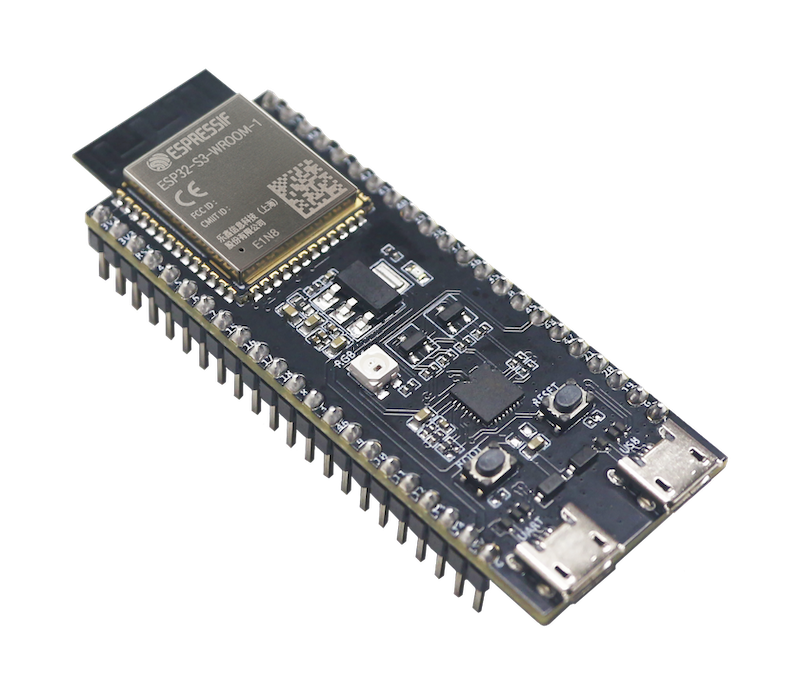
\includegraphics[width=0.5\linewidth,keepaspectratio]{gambar/esp32s3_devkitc1.png}
  \caption[\textit{Board} ESP32-S3-DevKitC-1]{\textit{Board} ESP32-S3-DevKitC-1~\cite{espressif_devkitc1}}
  \label{fig:esp32}
\end{figure}
% sumber gambar: https://docs.espressif.com/projects/esp-dev-kits/en/latest/esp32s3/_images/esp32-s3-devkitc-1-v1.1-isometric.png

ESP32-S3 menjadi satu-satunya perangkat \textit{edge} dalam penelitian ini dan menjalankan akuisisi sinyal AD8232, preprocessing, inferensi model INT8 melalui TensorFlow Lite for Microcontrollers, dan pengiriman MQTT. ESP32-S3 dipilih karena SRAM 512 KB jauh melebihi kebutuhan model INT8 sekitar 23 KB beserta \textit{tensor arena} sekitar 13 KB, PSRAM 8 MB dapat menampung antrean data selama koneksi terputus, dan WiFi sudah terintegrasi. Inferensi 1D-CNN INT8 bahkan telah berjalan pada mikrokontroler yang SRAM-nya jauh lebih kecil, seperti ARM Cortex-M4~\cite{kim_2023, sheeba_rani_2026} dan Arduino UNO 8-bit~\cite{zambrano_2026}. Sinyal AD8232 dicuplik melalui kanal ADC pertama karena ADC kedua tidak dapat dipakai bersamaan dengan WiFi~\cite{espressif_esp32s3_datasheet}.
% sumber: model/artifacts/metrics/fase7_delta.csv (ukuran_kb 22.94); model/CLAUDE.md HW-1 (arena 12.948 B), HW-6 (backlog 27.000 beat di PSRAM); firmware/include/perangkat.h (KANAL_EKG = ADC1_CHANNEL_0)

\subsection{Modul Sensor AD8232}
\label{subsec:ad8232}

AD8232 adalah \textit{front-end} analog terintegrasi untuk akuisisi sinyal ECG \textit{single-lead}. Chip ini memuat penguat instrumentasi \textit{low-noise}, filter \textit{high-pass} untuk meredam \textit{baseline wander}, filter \textit{low-pass} untuk meredam \textit{high-frequency noise}, serta deteksi lepasnya elektroda (\textit{lead-off detection})~\cite{analog_ad8232}. Keluarannya berupa sinyal analog yang dapat dicuplik langsung oleh ADC mikrokontroler. Modul AD8232 beserta elektrodanya ditunjukkan pada Gambar~\ref{fig:ad8232}.

\begin{figure}[!ht]
  \centering
  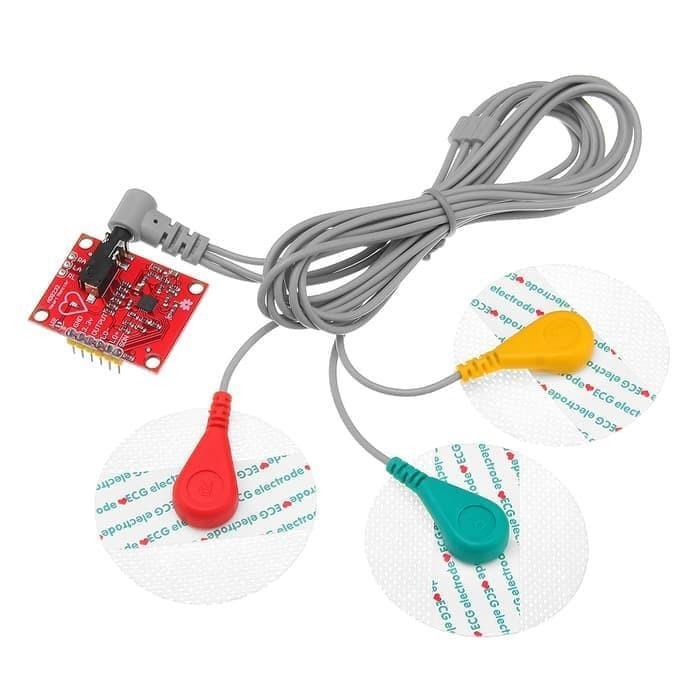
\includegraphics[width=0.55\linewidth,keepaspectratio]{gambar/gambar_2_2.png}
  \caption{Modul sensor AD8232 beserta elektroda \textit{wet-gel} tiga sadapan}
  \label{fig:ad8232}
\end{figure}

Dalam penelitian ini, AD8232 digunakan untuk menangkap sinyal ECG melalui tiga elektroda pada sadapan \textit{Modified Lead II} (MLII), karena gelombang R pada sadapan ini paling tinggi sehingga andal untuk deteksi R-\textit{peak}. Modul ini dipilih karena penguatan dan penyaringan sinyalnya sudah terintegrasi, keluarannya dapat langsung dicuplik ADC ESP32-S3, dan modul yang sama dipakai pada penelitian terkait yang menjadi pembanding~\cite{zambrano_2026, mulyawan_2026}.

\subsection{Layar TFT ST7789}
\label{subsec:tft-st7789}

ST7789 adalah \textit{controller} sekaligus \textit{driver} tunggal untuk layar TFT LCD 262 ribu warna dengan memori bingkai (\textit{frame memory}) internal berukuran 240$\times$320 piksel, sehingga mikrokontroler hanya perlu mengirim data piksel untuk area yang berubah. Chip ini menerima data melalui antarmuka paralel, RGB, maupun SPI tiga atau empat jalur~\cite{sitronix_st7789v3}. Contoh modul layar TFT 1,47 inci dengan \textit{driver} ST7789 ditunjukkan pada Gambar~\ref{fig:tft-st7789}.

\begin{figure}[!ht]
  \centering
  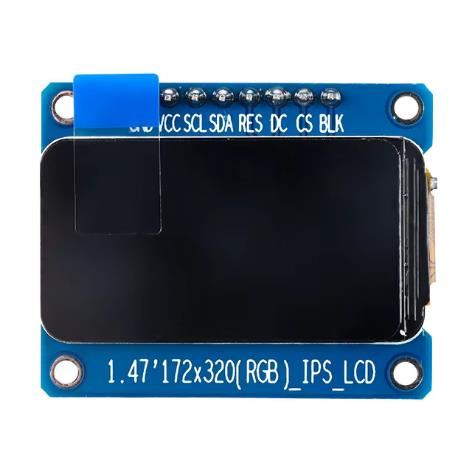
\includegraphics[width=0.4\linewidth,keepaspectratio]{gambar/modul_tft_st7789_mulyawan.png}
  \caption[Modul layar TFT 1,47 inci dengan \textit{driver} ST7789]{Modul layar TFT 1,47 inci dengan \textit{driver} ST7789~\cite{mulyawan_2026}}
  \label{fig:tft-st7789}
\end{figure}
% sumber gambar: Gambar 2.6 buku PA Mulyawan 2026 (pdfimages hlm. 43, 472x472 px)

Dalam penelitian ini, layar TFT 1,47 inci beresolusi 172$\times$320 piksel dengan \textit{driver} ST7789 digunakan untuk menampilkan laju jantung, gelombang ECG, waktu, status perekaman, dan menu. Layar ini dipilih karena ukurannya ringkas untuk perangkat yang dikenakan, resolusinya cukup untuk menampilkan gelombang ECG, dan antarmuka SPI hanya membutuhkan sedikit pin.

\subsection{Modul \textit{Buzzer} Pasif}
\label{subsec:buzzer-pasif}

\textit{Buzzer} pasif, atau \textit{buzzer} transduser, tidak memiliki rangkaian penggerak internal sehingga harus digerakkan gelombang kotak dari luar, dan frekuensi bunyinya mengikuti frekuensi gelombang tersebut. Sebaliknya, \textit{buzzer} aktif atau \textit{buzzer} indikator berbunyi pada satu frekuensi tetap begitu diberi tegangan searah~\cite{cui_buzzer_basics}. Contoh modul \textit{buzzer} pasif tiga pin dengan transistor penggerak ditunjukkan pada Gambar~\ref{fig:buzzer-pasif}.

\begin{figure}[!ht]
  \centering
  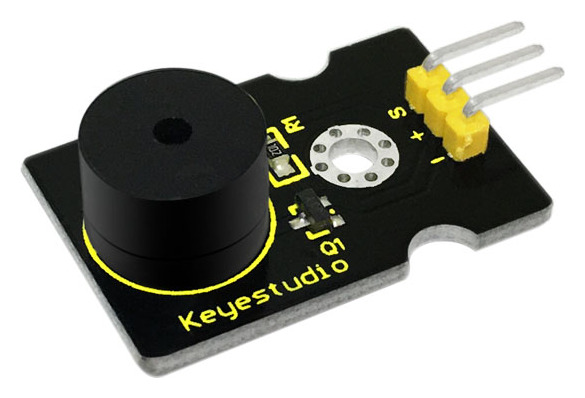
\includegraphics[width=0.45\linewidth,keepaspectratio]{gambar/modul_buzzer_pasif.jpg}
  \caption[Modul \textit{buzzer} pasif tiga pin]{Modul \textit{buzzer} pasif tiga pin~\cite{keyestudio_ks0019}}
  \label{fig:buzzer-pasif}
\end{figure}
% sumber gambar: https://wiki.keyestudio.com/images/a/af/KS0019_%284%29.jpg (dipotong tepinya)

Dalam penelitian ini, modul \textit{buzzer} pasif tiga pin dengan transistor penggerak digunakan sebagai indikator bunyi. \textit{Buzzer} pasif dipilih karena gelombang kotaknya dapat dibangkitkan periferal PWM ESP32-S3, sehingga nada dapat diatur dan satu bip dapat dibunyikan untuk setiap detak.

\subsection{Protokol MQTT}
\label{subsec:mqtt}

MQTT (\textit{Message Queuing Telemetry Transport}) adalah protokol komunikasi \textit{publish-subscribe} yang dirancang untuk perangkat IoT dengan \textit{overhead} \textit{header} minimal (2 byte) sehingga efisien dalam penggunaan \textit{bandwidth}~\cite{oasis_mqtt5}. MQTT mendukung tiga tingkat \textit{Quality of Service}, yaitu QoS-0 (\textit{at most once}), QoS-1 (\textit{at least once}), dan QoS-2 (\textit{exactly once}). Pada aplikasi kesehatan berbasis MQTT, QoS-1 menjadi kompromi terbaik antara latensi \textit{end-to-end} yang rendah dan variasi latensi yang kecil~\cite{akshatha_2022}. Dalam penelitian ini, MQTT digunakan untuk mengirim hasil klasifikasi per detak dari ESP32-S3 ke \textit{broker} ThingsBoard pada QoS-1, dan duplikat akibat pengiriman ulang dikenali di sisi \textit{cloud}.

\subsection{Platform Dashboard ThingsBoard}
\label{subsec:thingsboard}

ThingsBoard adalah platform IoT \textit{open-source} yang menyediakan
infrastruktur lengkap untuk pengumpulan, pemrosesan, visualisasi, dan
manajemen data perangkat IoT. Platform ini mendukung penerimaan data dari
perangkat melalui protokol MQTT secara langsung, menyimpannya dalam basis
data telemetri, dan menampilkannya melalui \textit{dashboard} yang dapat
dikonfigurasi sepenuhnya~\cite{reoukadji_2025}.

ThingsBoard Community Edition (CE) dapat di-\textit{host} secara mandiri
(\textit{self-hosted}). Arsitekturnya terdiri dari tiga komponen utama, yaitu
\textit{broker} MQTT terintegrasi yang menerima data telemetri dari perangkat,
mesin penyimpanan telemetri berbasis \textit{time-series} untuk rekaman
historis, dan \textit{dashboard engine} berbasis WebSocket. \textit{Dashboard
engine} memperbarui tampilan secara otomatis setiap paket baru diterima
sehingga menghasilkan perilaku \textit{real-time} dengan interval pembaruan
$\approx$1 detik tanpa perlu \textit{refresh} halaman. Tampilan antarmuka
ThingsBoard CE ditunjukkan pada Gambar~\ref{fig:thingsboard}.

\begin{figure}[H]
  \centering
  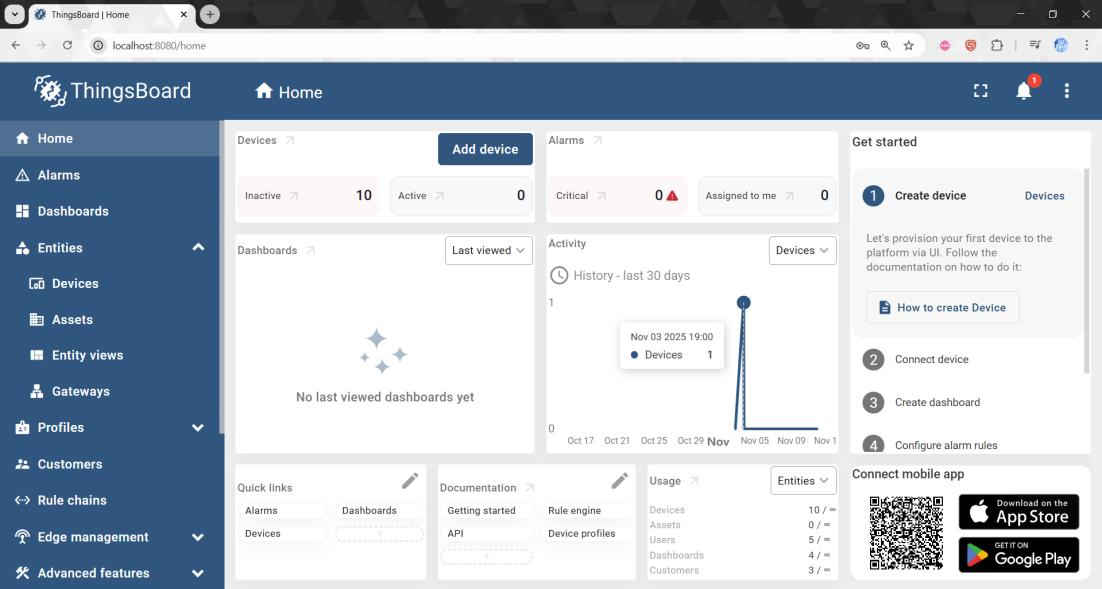
\includegraphics[width=0.92\linewidth,keepaspectratio]{gambar/gambar_2_3.png}
  \caption{Tampilan antarmuka platform ThingsBoard Community Edition}
  \label{fig:thingsboard}
\end{figure}

Sistem \textit{widget} ThingsBoard berbasis \textit{telemetry key} memungkinkan
setiap \textit{field} dalam payload JSON dari perangkat dipetakan ke komponen
visualisasi yang sesuai tanpa memerlukan pemrograman \textit{frontend}.
Contohnya adalah \textit{value card} untuk BPM, \textit{status badge} berwarna
untuk hasil klasifikasi, dan \textit{time-series chart} untuk tren laju jantung.
ThingsBoard juga menyediakan \textit{alarm rule engine} yang dapat dikonfigurasi
untuk memicu notifikasi otomatis ketika kondisi tertentu terpenuhi, misalnya
ketika label = 1 (Aritmia terdeteksi). Dalam penelitian ini, ThingsBoard CE
\textit{self-hosted} digunakan sebagai \textit{broker} MQTT sekaligus
\textit{dashboard} pemantauan hasil klasifikasi dari ESP32-S3.

\subsection{MIT-BIH \textit{Arrhythmia Database}}
\label{subsec:mitbih}

% NOTE: sloppypar dipakai karena "elektrokardiogram" bikin overfull hbox
\begin{sloppypar}
MIT-BIH \textit{Arrhythmia Database} merupakan basis data rekaman
elektrokardiogram standar yang dikembangkan melalui kolaborasi antara
Massachusetts Institute of Technology dan Beth Israel Hospital (BIH) sejak
awal tahun 1980-an. Basis data ini berisi 48 rekaman ECG dua kanal dari
47 subjek, masing-masing berdurasi sekitar 30 menit, yang dicuplik pada
frekuensi 360 Hz dengan resolusi 11-bit pada rentang $\pm$5 mV. Kanal
utama yang digunakan adalah modifikasi sadapan Lead II (MLII), yang
merupakan kanal yang sama dengan konfigurasi sensor pada penelitian
ini~\cite{moody_mark_2001}.
\end{sloppypar}

Keseluruhan rekaman telah dianotasi secara manual oleh kardiolog ahli,
menandai lokasi dan jenis setiap detak jantung. Anotasi ini menggunakan
sistem simbol standar AAMI (\textit{Association for the Advancement of
Medical Instrumentation}) yang mencakup lebih dari 15 jenis detak.
Di antaranya terdapat detak sinus normal (N), kontraksi ventrikular
prematur (V), dan detak supraventrikular (S). Tingkat anotasi per-detak inilah yang
menjadikan MIT-BIH sebagai \textit{benchmark} utama untuk evaluasi
algoritma deteksi aritmia secara global~\cite{moody_mark_2001}. Contoh rekaman beserta anotasinya ditunjukkan pada Gambar~\ref{fig:mitbih-ecg}.

\begin{figure}[H]
  \centering
  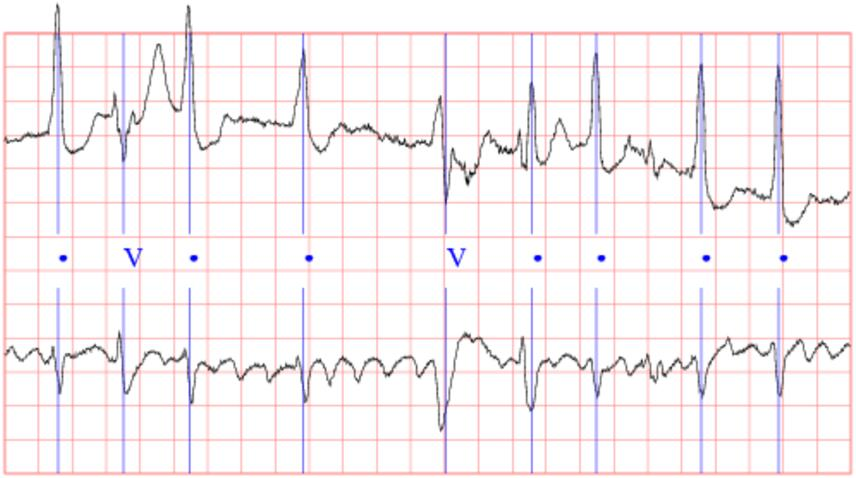
\includegraphics[width=0.90\linewidth,keepaspectratio]{gambar/gambar_2_4.png}
  \caption{Contoh visualisasi rekaman ECG dua kanal dari MIT-BIH
           \textit{Arrhythmia Database} beserta anotasi per-detak,
           dengan simbol ``V'' menunjukkan kontraksi ventrikular prematur (PVC)
           dan simbol titik menunjukkan detak normal}
  \label{fig:mitbih-ecg}
\end{figure}

Dalam penelitian ini, MIT-BIH \textit{Arrhythmia Database} digunakan
sebagai sumber data untuk dua keperluan yang berbeda. Model CNN dilatih
dengan rekaman dari separuh kelompok pasien (DS1) dan diuji dengan rekaman
dari kelompok pasien yang berbeda sepenuhnya (DS2), yang dikenal sebagai
pembagian \textit{inter-patient}.
Strategi ini memastikan bahwa performa model yang diukur mencerminkan
kemampuan generalisasi terhadap pasien baru yang tidak pernah dilihat
selama pelatihan, dan bukan sekadar hafalan pola dari pasien yang sama.

\subsection{Simulasi \textit{Error} Deteksi R-\textit{peak} dengan \textit{Jitter}}
\label{subsec:augmentasi-jitter}

Klasifikasi per detak memotong sinyal ECG menjadi \textit{window} di sekitar puncak R. Pada MIT-BIH posisi tersebut berasal dari anotasi kardiolog, sedangkan pada perangkat posisi itu dihasilkan detektor R-\textit{peak} yang dapat meleset, sehingga evaluasi dengan posisi anotasi belum mewakili pemakaian nyata~\cite{dias_2021}. Dias et al.~\cite{dias_2021} mensimulasikan \textit{error} tersebut dengan \textit{jitter}, yaitu menggeser setiap puncak R menjadi $r'_i = r_i + u_i$. Nilai $u_i$ diambil acak dari sebaran seragam pada rentang $\pm\delta$ sampel, lalu \textit{window} dipotong dan fitur R-R dihitung dari posisi baru. Batas $\delta = 18$ sampel setara dengan toleransi \textit{error} 50 ms pada studi kinerja detektor QRS. Pada batas tersebut, sensitivitas kelas N, S, dan V hanya turun dari 94,5\%, 92,5\%, dan 88,6\% menjadi 93,7\%, 89,7\%, dan 87,9\%~\cite{dias_2021}.
% sumber: Dias 2021 (CMPB 202:105948) sec. 4.2 hlm. 3 (uniform -delta..+delta, delta 0..18, 18 sampel = 50 ms, 128+127 sampel), sec. 4.3.1 (RR dari posisi tersegmentasi), sec. 5.2 hlm. 6 (33 ulangan), Tabel 3 hlm. 5 (Se N/S/V delta 0: 94,5/92,5/88,6; delta 18: 93,7/89,7/87,9)

Dias et al.\ memakai \textit{jitter} sebagai uji ketahanan. Dalam penelitian ini, \textit{jitter} dipakai sebagai augmentasi data latih dengan dua penyesuaian. Besar pergeseran diambil ulang dari sebaran \textit{error} detektor yang diukur sendiri pada DS1, karena sekitar 80\% deteksi hanya berselisih satu sampel atau kurang dari anotasi, sedangkan sebagian kecil lainnya menyimpang hingga puluhan sampel. Selain itu, setiap detak DS1 disertai salinan ber-\textit{jitter} di samping salinan bersihnya, sedangkan DS2 dibiarkan bersih sebagai data uji.
% sumber: model/docs/jitter-walkthrough.md bagian 2 (DS1 50.601 pasangan, 79,85% <=1 sampel, |p99| 26, maks 54); model/config.py (JITTER_MODEL = "empiris", JITTER_SALINAN = 2); model/scripts/prep_beats.py (1 bersih + 2 jitter, hanya DS1 mitdb)

\section{Penelitian Terkait}
\label{sec:penelitian-terkait}

\subsection{A Multistage Denoising Framework for Ambulatory ECG Signal Based on Domain Knowledge and Motion Artifact Detection}
\label{subsec:related-xie2021}

Xie et al.~\cite{xie_2021} mengusulkan kerangka preprocessing multi-tahap untuk sinyal ECG \textit{ambulatory}. Kerangka tersebut menggabungkan \textit{Frequency-Adaptive Noise Estimation} (FANE) berbasis \textit{wavelet} untuk menekan \textit{motion artifact}, \textit{Morphological Analysis and Detection} (MAD), \textit{Singular Value Thresholding} (SVT), serta \textit{Complete Ensemble Empirical Mode Decomposition} (CEEMD) untuk mengatasi \textit{baseline wander}. Kombinasi metode ini terbukti meningkatkan \textit{Signal-to-Noise Ratio} (SNR) sebesar 7\%--25\% dibandingkan metode konvensional pada \textit{dataset} ECG \textit{ambulatory}. Namun, seluruh eksperimen dilakukan pada perangkat PC server tanpa pelaporan latensi pemrosesan atau penggunaan memori. Penelitian tersebut memberikan referensi penting untuk memahami tantangan \textit{noise} pada ECG \textit{ambulatory}, sekaligus menunjukkan \textit{gap} bahwa algoritma preprocessing yang efektif belum divalidasi pada MCU \textit{low-power}.

Berbeda dengan penelitian tersebut yang menumpukan penekanan \textit{noise} pada CEEMD dan \textit{wavelet} yang beban komputasinya berat dan belum dikuantisasi untuk mikrokontroler, penelitian ini memakai filter Butterworth dan deteksi R-\textit{peak} Pan-Tompkins yang ringan. Pilihan itu diambil agar preprocessing dapat berjalan \textit{real-time} pada mikrokontroler hemat daya dan beban komputasinya terukur.

\subsection{A Real-Time Embedded System to Detect QRS-Complex and Arrhythmia Classification Using LSTM Through Hybridized Features}
\label{subsec:related-karri2023}

Karri dan Annavarapu~\cite{karri_2023} merancang sistem \textit{embedded} \textit{real-time} untuk deteksi kompleks QRS dan klasifikasi aritmia menggunakan pendekatan \textit{hybrid} yang menggabungkan \textit{Discrete Wavelet Transform} (DWT), \textit{Delta-Sigma Modulation} (DSM), dan model LSTM. Sistem DWT+DSM mampu mendeteksi kompleks QRS dalam 17,2 ms dengan konsumsi daya 680 nW pada chip DSM, dan diuji pada Raspberry Pi 4 (ARM Cortex-A72, RAM 4 GB). Meskipun berhasil menunjukkan kelayakan pemrosesan ECG secara \textit{embedded}, penggunaan Raspberry Pi 4 tidak mewakili batasan MCU \textit{low-power} yang sesungguhnya. \textit{Gap} pada penelitian tersebut adalah absennya implementasi dan validasi pada MCU kelas ESP32 atau Cortex-M4.

Berbeda dengan penelitian tersebut yang tidak mengukur daya total maupun RAM dan belum terhubung ke \textit{cloud}, penelitian ini menjalankan seluruh jalur pada mikrokontroler ESP32-S3 dan melaporkan beban komputasi serta memori yang terpakai di perangkat. Hasil klasifikasinya kemudian diteruskan ke \textit{cloud} melalui MQTT.

\subsection{Real-Time Fetal Arrhythmia Detection Using Deep Learning on an Embedded fECG Monitoring System}
\label{subsec:related-mekhfioui2025}

Mekhfioui et al.~\cite{mekhfioui_2025} mengembangkan sistem deteksi aritmia jantung janin berbasis sinyal fECG. Sistem tersebut memakai \textit{Independent Component Analysis} (ICA) untuk separasi sinyal, diikuti \textit{bandpass filtering} dan segmentasi ke dalam jendela 3 detik, serta klasifikasi menggunakan model 1D-CNN ringan yang diimplementasikan pada Raspberry Pi. Sistem mencapai akurasi 98,2\%, sensitivitas 98,8\%, dan F1-\textit{score} 98,1\% pada \textit{dataset} Kaggle dan NIFECGDB. Penelitian tersebut menjadi acuan arsitektur 1D-CNN untuk klasifikasi sinyal kardiovaskular pada \textit{embedded system}. Namun, implementasinya masih pada Raspberry Pi, dan ICA belum dievaluasi pada MCU dengan batasan RAM dan daya yang jauh lebih ketat.

Berbeda dengan penelitian tersebut yang memakai ICA yang sensitif terhadap \textit{noise}, penelitian ini memakai jalur preprocessing deterministik yang beban komputasinya diukur langsung di mikrokontroler.

\subsection{TinyML-Based Classification in an ECG Monitoring Embedded System}
\label{subsec:related-kim2023}

Kim et al.~\cite{kim_2023} mengusulkan TinyCES, sebuah model 1D-CNN terkuantisasi yang dirancang khusus untuk monitoring ECG pada perangkat \textit{embedded} dengan sumber daya terbatas. Model berhasil di-\textit{deploy} pada Arduino Nano 33 BLE Sense (ARM Cortex-M4) dengan ukuran model 27 KB dan akurasi klasifikasi biner sebesar 97\% menggunakan \textit{dataset} MIT-BIH dan PTB ECG. Penelitian tersebut merupakan salah satu dari sedikit studi yang benar-benar menjalankan inferensi ECG di MCU fisik \textit{low-power}. Namun, TinyCES masih terbatas pada klasifikasi biner dan tidak menyertakan laporan latensi inferensi, penggunaan RAM saat \textit{runtime}, maupun konsumsi daya aktual selama operasi kontinu.

Penelitian tersebut paling dekat dengan pendekatan penelitian ini. Berbeda dengan penelitian tersebut yang berhenti pada inferensi di perangkat, penelitian ini melengkapi inferensi INT8 di ESP32-S3 dengan pengukuran latensi dan memori di perangkat serta \textit{pipeline} \textit{edge-to-cloud} yang resilien, sedangkan klasifikasinya sama-sama biner.

\subsection{Designing Resilient IoT and Edge Computing with Federated TinyML}
\label{subsec:related-laiu2026}

Laiu et al.~\cite{laiu_2026} mengusulkan arsitektur DRIFT (\textit{Distributed Resilient IoT Federated TinyML}), sebuah kerangka tiga-lapisan yang mengintegrasikan TinyML dan \textit{Federated Learning} untuk meningkatkan keamanan dan ketahanan sistem IoT/MCU. Penelitian tersebut menunjukkan bahwa kuantisasi float32 ke INT8 menghasilkan kompresi model $4\times$ dengan degradasi akurasi kurang dari $0{,}01\%$, serta membuktikan bahwa beban komputasi pada MCU dapat dikurangi melalui preprocessing terdistribusi di lapisan \textit{edge}. Fokus penelitian tersebut adalah pada keamanan siber IoT, bukan pada monitoring sinyal biomedis, dan evaluasinya dilakukan secara simulasi tanpa pengujian \textit{streaming} data ECG kontinu pada \textit{hardware} MCU fisik.

Berbeda dengan penelitian tersebut yang mengevaluasi kuantisasi pada deteksi intrusi jaringan secara simulasi, penelitian ini menerapkan kuantisasi INT8 pada model deteksi aritmia. Selisih metrik dan latensinya diukur langsung di ESP32-S3 dengan \textit{streaming} ECG kontinu.

\subsection{Implementing TinyML in Internet of Things Devices: A Systematic Literature Review}
\label{subsec:related-solispino2026}

Solis Pino et al.~\cite{tinyml_iot_review} melakukan tinjauan literatur sistematis terhadap 114 studi primer tentang implementasi TinyML pada perangkat IoT menggunakan protokol PRISMA dan strategi pencarian multi-\textit{database}. Hasil \textit{review} mengungkapkan bahwa CNN adalah arsitektur yang paling sering digunakan, ESP32 dan Arduino Nano 33 BLE Sense adalah platform \textit{hardware} yang paling umum, serta \textit{healthcare} adalah domain aplikasi yang paling banyak diteliti. Tinjauan ini juga mengidentifikasi tantangan utama yang belum terselesaikan, meliputi keterbatasan memori/CPU, kerentanan keamanan, dan absennya standardisasi implementasi TinyML antar platform.

Berbeda dengan tinjauan tersebut yang memetakan praktik lintas studi tanpa eksperimen, penelitian ini memakai temuannya sebagai dasar pemilihan CNN, ESP32, dan TFLite Micro, lalu menguji pilihan itu secara eksperimental pada satu perangkat.

\subsection{Advanced IoT-Enabled Embedded Wearable System for Continuous Cardiovascular Health Monitoring Using Edge Intelligence}
\label{subsec:related-sheebarani2026}

Sheeba Rani et al.~\cite{sheeba_rani_2026} mengusulkan sistem \textit{wearable} monitoring kardiovaskular kontinu yang mengimplementasikan model \textit{hybrid} 1D-TA-DSC (kombinasi 1D \textit{Depthwise Separable Convolution} dan \textit{Temporal Attention}-GRU) pada ARM Cortex-M4 menggunakan TFLite. Setelah kuantisasi \textit{post-training}, model dikompres dari 22 KB menjadi 11 KB dengan latensi inferensi 7 ms, akurasi 99,8\%, dan AUROC 0,997 pada \textit{dataset} MIMIC-III (rekaman ICU). Penelitian tersebut adalah salah satu yang paling detail dalam melaporkan metrik \textit{hardware} untuk monitoring kardiovaskular di MCU. Namun, penelitian tersebut tidak menyertakan evaluasi konsumsi daya pada kondisi operasi kontinu maupun mekanisme resiliensi \textit{pipeline} \textit{edge-to-cloud}.

Berbeda dengan penelitian tersebut yang dilatih pada rekaman ICU MIMIC-III yang belum tentu mewakili kondisi \textit{ambulatory}, penelitian ini dilatih dan diuji secara \textit{inter-patient} pada MIT-BIH. Penelitian ini juga menambahkan \textit{pipeline} \textit{edge-to-cloud} yang resilien yang tidak dibahas pada penelitian tersebut.

\subsection{An On-Device Machine Learning Assisted System for Unobtrusive Cardiac Auscultation}
\label{subsec:related-chowdhury2023}

Chowdhury dan Chattopadhyay~\cite{chowdhury_2023} mengembangkan sistem auskultasi jantung berbasis \textit{on-device machine learning} yang diimplementasikan pada Arduino Nano 33 BLE Sense (ARM Cortex-M4, 64 MHz) untuk klasifikasi suara jantung secara \textit{real-time} tanpa koneksi internet. Sistem melaporkan latensi \textit{pipeline} DSP sebesar 23,19 ms untuk ekstraksi fitur MFCC, dengan konsumsi arus puncak 8,6 mA pada 3,3 V (sekitar 28,38 mW) dan daya tahan baterai 11,5 jam menggunakan baterai 240 mAh. Penelitian tersebut memberikan referensi \textit{benchmark} konsumsi daya aktual untuk \textit{inference on-device} pada MCU Cortex-M4, meskipun fokusnya pada auskultasi suara jantung, bukan sinyal ECG.

Berbeda dengan penelitian tersebut yang mengolah suara jantung (PCG), penelitian ini mengolah sinyal ECG dengan jalur inferensi yang serupa di perangkat.

\subsection{AI-Powered Anomaly Detection and Cybersecurity in Healthcare IoT with Fog/Edge}
\label{subsec:related-alquayed2026}

Al-Quayed~\cite{al_quayed_2026} mengusulkan kerangka FE-ACS yang mendistribusikan pemrosesan dan deteksi anomali ke lapisan \textit{fog} dan \textit{edge} pada ekosistem IoT kesehatan. Pengukuran performa menunjukkan bahwa arsitektur \textit{fog-edge} mencapai latensi total rata-rata 18,7 ms dibandingkan 152,3 ms pada arsitektur \textit{cloud-centric}, mempresentasikan peningkatan 87,7\% dengan efisiensi \textit{bandwidth} $8{,}5\times$ lebih tinggi. Penelitian tersebut membuktikan secara kuantitatif keunggulan arsitektur \textit{edge} atas \textit{cloud-centric} untuk aplikasi IoT kesehatan. Namun, fokus penelitian tersebut adalah pada keamanan siber, bukan pada \textit{streaming} data ECG kontinu, dan tidak membahas mekanisme resiliensi saat koneksi terputus.

Berbeda dengan penelitian tersebut yang mengukur keunggulan latensi \textit{fog-edge} untuk deteksi anomali keamanan, penelitian ini memakai bukti kuantitatif itu sebagai dasar pemindahan inferensi ke perangkat. Penelitian ini juga menambahkan mekanisme bufer lokal untuk \textit{streaming} ECG saat koneksi terputus.

\subsection[Resilient Edge-to-Cloud Architecture with Self-Healing and Self-Correcting Mechanisms for Industrial Data Continuity]{Resilient Edge-to-Cloud Architecture with Self-Healing and\\ Self-Correcting Mechanisms for Industrial Data Continuity}
\label{subsec:related-boluda2026}

Boluda-Prieto et al.~\cite{resilient_edge_cloud} mengusulkan arsitektur E2C (\textit{Edge-to-Cloud}) berbasis \textit{microservices} dengan mekanisme \textit{self-healing} dan \textit{self-correcting} menggunakan \textit{stack} Kubernetes, Rancher, Prometheus, Grafana, dan Node-RED. Sistem menggunakan MQTT sebagai protokol transmisi dengan mekanisme \textit{edge buffering} yang mempertahankan \textit{Recovery Point Objective} (RPO) mendekati nol untuk aliran data kritis saat terjadi saturasi jaringan. Pengujian \textit{stress test} dengan kondisi \textit{overload} CPU dan saturasi jaringan menunjukkan kemampuan sistem mendeteksi \textit{threshold}, melakukan \textit{scaling}, dan mengisolasi \textit{node} bermasalah secara otomatis. Meskipun prinsip resiliensi pada penelitian tersebut relevan untuk \textit{streaming} ECG, seluruh implementasi berfokus pada data \textit{time-series} industri manufaktur dan menggunakan infrastruktur berbasis Kubernetes yang terlalu berat untuk MCU \textit{low-power}.

Berbeda dengan arsitektur tersebut yang mengandalkan \textit{microservices} Kubernetes di sisi server, penelitian ini menerapkan prinsip \textit{edge buffering} yang sama di dalam mikrokontroler. \textit{Ring buffer} di PSRAM ESP32-S3 menahan detak saat koneksi terputus dan mengurasnya saat koneksi pulih.

\subsection{Real-Time Cardiac Arrhythmia Classification Using TinyML on
Ultra-Low-Cost Microcontrollers}
\label{subsec:related-zambrano2026}

Zambrano-de la Torre et al.~\cite{zambrano_2026} menunjukkan klasifikasi aritmia \emph{real-time} menggunakan
1D-CNN terkuantisasi INT8 yang di-\emph{deploy} pada mikrokontroler Arduino UNO 8-bit
(ATmega328P, SRAM 2 KB, Flash 32 KB). Sistemnya mengintegrasikan akuisisi sinyal ECG
dengan \emph{front-end} analog AD8232, filter Butterworth \emph{bandpass} 0,5--40 Hz,
deteksi R-peak Pan-Tompkins, segmentasi \emph{window} 250 sampel (sekitar 0,7 detik
pada 360 Hz), hingga visualisasi pada layar OLED. Model dilatih dan dievaluasi pada
MIT-BIH Arrhythmia Database untuk tiga kelas (Normal, Ventrikular, Supraventrikular).
Model yang dihasilkan berukuran di bawah 22 KB dengan latensi inferensi sekitar 200 ms
per detak dan degradasi akurasi kurang dari 0,7\% akibat kuantisasi INT8. Validasi
dilakukan melalui dua jalur terpisah, yaitu evaluasi model pada dataset \emph{benchmark}
dan uji fungsional \emph{real-time} menggunakan relawan sehat tanpa penegakan diagnosis
klinis. Penelitian tersebut memberikan bukti kelayakan bahwa \textit{pipeline}
akuisisi--preprocessing--inferensi INT8 dapat berjalan pada mikrokontroler yang
jauh lebih terbatas dari ESP32-S3. Namun, pembagian datanya dilakukan per-detak tanpa
pemisahan antarpasien, sehingga metriknya berpotensi optimistis.

Berbeda dengan penelitian tersebut yang membagi data per detak dan tidak memakai
cabang ritme, penelitian ini mengadopsi skema antarpasien (\emph{inter-patient},
DS1/DS2) yang lebih ketat untuk mengukur generalisasi. Penelitian ini juga menambahkan
cabang ritme berbasis interval R-R, dan perangkatnya dilengkapi \textit{pipeline}
\textit{edge-to-cloud} yang resilien yang tidak ada pada penelitian tersebut.

\subsection{Rancang Bangun Smart Wearables Terintegrasi IoT untuk Deteksi Dini
Atrial Fibrilasi Menggunakan SVM Berbasis Cloud}
\label{subsec:related-mulyawan2026}

Mulyawan~\cite{mulyawan_2026} merancang perangkat \emph{wearable} berbasis ESP32 yang mengintegrasikan
sensor EKG AD8232, sensor SpO\textsubscript{2} MAX30102, dan sensor suhu MLX90614 untuk
deteksi dini atrial fibrilasi (AFib). Deteksi puncak R dan ekstraksi fitur interval RR
dilakukan di sisi \emph{edge}, kemudian fitur ditransmisikan via MQTT ke infrastruktur
\emph{cloud} lokal berbasis ThingsBoard Community Edition dan basis data PostgreSQL.
Klasifikasi dilakukan oleh model Support Vector Machine (SVM) dengan kernel Radial Basis
Function yang \emph{di-deploy pada sisi backend}, dilatih menggunakan dataset MIT-BIH dan
mencapai akurasi tinggi pada pengujian \emph{offline}.
Gambar~\ref{fig:alat-mulyawan} menampilkan \emph{prototype} perangkat yang dihasilkan.

\begin{figure}[H]
  \centering
  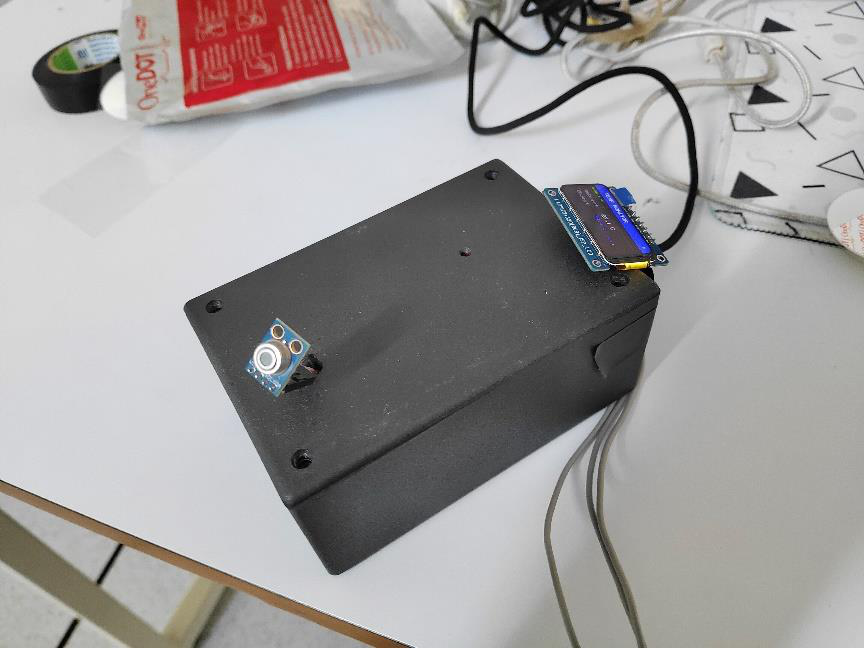
\includegraphics[width=0.7\linewidth]{gambar/gambar_alat_terdahulu_mulyawan.png}
  \caption{\emph{Prototype} perangkat \emph{wearable} pada penelitian
  terdahulu~\cite{mulyawan_2026}, berupa integrasi ESP32 dan sensor AD8232/MAX30102/MLX90614 dalam \emph{blackbox}}
  \label{fig:alat-mulyawan}
\end{figure}

Penelitian tersebut merupakan pendahulu langsung dari penelitian ini dengan platform
sensor dan \emph{dashboard} yang sama, dan penelitian ini melanjutkan rancangan tersebut
pada lokasi inferensi yang berbeda. Berbeda dengan penelitian tersebut yang menjalankan
klasifikasi secara terpusat di \emph{cloud} sehingga pengambilan keputusan tetap
bergantung pada ketersediaan koneksi, penelitian ini memindahkan inferensi sepenuhnya ke
perangkat (\emph{on-device}) menggunakan CNN terkuantisasi INT8. Selain itu, penelitian
ini menambahkan mekanisme resiliensi \emph{pipeline} saat koneksi terputus yang belum
disertakan pada penelitian terdahulu.

\subsection{Perbandingan Penelitian Terkait}
\label{subsec:perbandingan-penelitian}

Berdasarkan ulasan kedua belas penelitian tersebut, Tabel~\ref{tab:perbandingan-penelitian} merangkum perbandingan metode, platform, dan perbedaan utama setiap penelitian terhadap penelitian ini.

{\scriptsize
\setlength{\tabcolsep}{3pt}
\renewcommand{\arraystretch}{1.2}
\begin{longtable}{|c|L{3.5cm}|L{2.0cm}|L{2.0cm}|L{1.8cm}|L{2.8cm}|}
\caption{Perbandingan Penelitian Terkait}\label{tab:perbandingan-penelitian}\\
\hline
\textbf{No} & \textbf{Judul (Tahun)} & \textbf{Penyakit / Domain} & \textbf{Metode (Model)} & \textbf{Platform Komputasi} & \textbf{Perbedaan} \\ \hline
\endfirsthead
\hline
\textbf{No} & \textbf{Judul (Tahun)} & \textbf{Penyakit / Domain} & \textbf{Metode (Model)} & \textbf{Platform Komputasi} & \textbf{Perbedaan} \\ \hline
\endhead
\endfoot
\endlastfoot

1 & \textit{A multi-stage denoising framework for ambulatory ECG signal based on domain knowledge and motion artifact detection} (2021) & Preprocessing sinyal ECG (penekanan noise) & FANE+MAD, SVT, CEEMD, wavelet (denoising bertingkat) & PC server (offline) & \textit{Denoising} bertingkat efektif (SNR naik 7--25\%), tetapi hanya dievaluasi di PC server dan belum diuji pada mikrokontroler. \\ \hline

2 & \textit{A real-time embedded system to detect QRS-complex and arrhythmia classification using LSTM through hybridized features} (2023) & Aritmia & DWT + Delta-Sigma Modulation + LSTM & Raspberry Pi 4 & Akurasi 99,6\% dan \textit{real-time} di Raspberry Pi 4, yang bukan MCU \textit{low-power}, tanpa integrasi \textit{cloud}. \\ \hline

3 & \textit{Real-time fetal arrhythmia detection using deep learning on an embedded fECG monitoring system} (2025) & Aritmia janin (\textit{fetal}) & Bandpass + ICA + 1D-CNN ringan & Raspberry Pi 4 & 1D-CNN ringan dengan transmisi Wi-Fi di Raspberry Pi, ICA belum dievaluasi di MCU dan daya tidak dilaporkan. \\ \hline

4 & \textit{TinyML-Based Classification in an ECG Monitoring Embedded System} (2023) & Aritmia (klasifikasi biner normal/\allowbreak abnormal) & 1D-CNN INT8 (TFLM, \textit{Post-Training Quantization}) & Arduino Nano BLE (Cortex-M4) & Inferensi \textit{on-device} INT8 (\textasciitilde27 KB, akurasi \textasciitilde97\%), terdekat dengan pendekatan ini, tetapi tanpa laporan latensi, daya, dan \textit{pipeline} resilien. \\ \hline

5 & \textit{Designing resilient IoT and Edge Computing with federated TinyML} (2026) & --- (keamanan jaringan IoT) & \textit{Federated Learning} + kuantisasi MLP INT8 & Testbed/\allowbreak simulasi & Kuantisasi float32$\rightarrow$INT8 (kompresi 4$\times$, akurasi turun $<$0,01\%) pada deteksi intrusi jaringan, tanpa \textit{benchmark} MCU fisik. \\ \hline

6 & \textit{Implementing TinyML in Internet of Things devices: A systematic literature review} (2026) & --- (tinjauan literatur, 114 studi) & SLR (PRISMA) & Berbagai (MCU + SBC) & Tinjauan literatur, bukan eksperimen, memetakan algoritma, \textit{hardware}, dan tantangan TinyML (memori, CPU, standardisasi). \\ \hline

7 & \textit{Advanced IoT-enabled embedded wearable system for continuous cardiovascular health monitoring using edge intelligence} (2026) & Penyakit kardio\-vaskular / aritmia (4 kelas keparahan) & 1D Depthwise-\allowbreak Separable Conv + Temporal Attention-\allowbreak GRU (INT8 PTQ) & ARM Cortex-M4 (STM32\-F407) & Inferensi \textasciitilde7 ms dengan model \textasciitilde11 KB di Cortex-M4, tetapi dilatih pada data ICU (MIMIC-III) dan tanpa \textit{pipeline} resilien. \\ \hline

8 & \textit{An on-device machine learning assisted system for unobtrusive cardiac auscultation} (2023) & Kelainan jantung (auskultasi/\allowbreak PCG) & DSP + MFCC + ML \textit{on-device} & Arduino Nano BLE & Berhasil menjalankan ML \textit{on-device}, tetapi memproses sinyal suara jantung (PCG), bukan sinyal ECG. \\ \hline

9 & \textit{AI-Powered Anomaly Detection and Cybersecurity in Healthcare IoT with Fog/Edge} (2026) & Keamanan siber IoT kesehatan & Kerangka FE-ACS (deteksi anomali \textit{fog-edge}) & Arsitektur \textit{fog/edge} IoT & Latensi \textit{fog-edge} 18,7 ms vs 152,3 ms \textit{cloud-centric}, tetapi berfokus keamanan siber, tanpa resiliensi putus koneksi. \\ \hline

10 & \textit{Resilient Edge-to-Cloud Architecture with Self-Healing and Self-Correcting Mechanisms for Industrial Data Continuity} (2026) & Kontinuitas data industri & E2C \textit{microservices} + MQTT + \textit{edge buffering} (\textit{self-healing}) & Kubernetes (Rancher, Prometheus, Grafana) & RPO mendekati nol saat saturasi jaringan, tetapi untuk data industri dengan Kubernetes yang terlalu berat bagi MCU. \\ \hline

11 & \textit{Real-Time Cardiac Arrhythmia Classification Using TinyML on Ultra-Low-Cost Microcontrollers} (2026) & Aritmia (3 kelas: N/V/S) & 1D-CNN INT8 (TFLM, PTQ) + AD8232 & Arduino UNO 8-bit (ATmega328P) & Jalur AD8232 ke inferensi INT8 (model $<$22 KB) berjalan di MCU 8-bit, tetapi data dibagi per detak, tanpa \textit{pipeline} resilien. \\ \hline

12 & \textit{Rancang Bangun Smart Wearables Terintegrasi IoT untuk Deteksi Dini Atrial Fibrilasi Menggunakan SVM Berbasis Cloud} (2026) & Atrial fibrilasi & Fitur RR + SVM (RBF) & ESP32 (akuisisi) + SVM di cloud & Pendahulu langsung dengan sensor dan \textit{dashboard} sama, tetapi inferensi di \textit{cloud}, tanpa kuantisasi di MCU maupun resiliensi \textit{pipeline}. \\ \hline

13 & \textit{Implementasi Sistem Monitoring Detak Jantung Kontinu Berbasis IoT Edge Computing untuk Deteksi Dini Aritmia} (penelitian ini) & Aritmia (deteksi dini) & Preprocessing di MCU (Butterworth + Pan-Tompkins) + 1D-CNN INT8 + fitur RR (\textit{hybrid}) \textit{on-device} ($\pm$23 KB) & \textit{ESP32-S3 (inferensi on-device)} & Preprocessing \textit{real-time}, inferensi CNN INT8, dan \textit{pipeline} resilien (\textit{ring buffer} lokal + MQTT) menyatu dalam satu ESP32-S3. \\ \hline
% sumber: model/artifacts/metrics/fase7_delta.csv (ukuran_kb 22.94)

\end{longtable}
}

Tabel~\ref{tab:perbandingan-penelitian} memperlihatkan bahwa belum ada penelitian yang menyatukan ketiga aspek sekaligus. Ketiga aspek itu adalah preprocessing ECG yang divalidasi di MCU \textit{low-power}, inferensi TinyML \textit{on-device}, serta \textit{pipeline} \textit{edge-to-cloud} dengan resiliensi berbasis MQTT dan bufer lokal. Kelompok pertama mengevaluasi metodenya di PC server atau secara simulasi, yaitu kerangka \textit{denoising} multi-tahap~\cite{xie_2021} dan kuantisasi pada deteksi intrusi~\cite{laiu_2026}, sehingga beban komputasi dan memorinya di mikrokontroler belum diketahui. Kelompok kedua sudah berjalan di perangkat \textit{embedded}, tetapi memakai Raspberry Pi~\cite{karri_2023} atau infrastruktur Kubernetes~\cite{resilient_edge_cloud} yang jauh lebih berat daripada MCU, atau berhenti pada inferensi di MCU tanpa \textit{pipeline} \textit{edge-to-cloud} yang resilien~\cite{kim_2023}.

Penelitian ini memilih ESP32-S3 sebagai satu perangkat yang menjalankan preprocessing, inferensi CNN INT8, dan bufer lokal MQTT. Pilihan itu disadari membawa keterbatasan, yaitu klasifikasi biner, uji \textit{pipeline} dengan sumber sinyal \textit{replay}, dan subjek sehat non-klinis. Angka akurasi pada sebagian penelitian tersebut juga tidak dapat dibandingkan secara langsung dengan hasil penelitian ini. Zambrano-de la Torre et al.\ membagi data per detak tanpa pemisahan antarpasien sehingga metriknya berpotensi optimistis~\cite{zambrano_2026, xiao_2023}, sedangkan penelitian pendahulu menyasar deteksi atrial fibrilasi dan melaporkan akurasi pada pengujian \textit{offline}~\cite{mulyawan_2026}. Penelitian ini menggunakan skema \textit{inter-patient} dengan metrik \textit{recall}, \textit{precision}, \textit{specificity}, F1, dan AUC. Kontribusinya karena itu bukan akurasi yang lebih unggul, melainkan evaluasi yang lebih ketat terhadap generalisasi pada pasien baru beserta kinerja yang terukur di perangkat.

\chapter{Deskripsi Sistem}
\label{chap:deskripsi-sistem}

\section{Deskripsi Solusi}
\label{sec:deskripsi-solusi}

Sistem pemantauan detak jantung berbasis IoT pada umumnya mengirimkan sinyal mentah secara langsung ke server \textit{cloud} untuk diproses~\cite{kim_2023, escobedo_2026}. Pendekatan terpusat ini menimbulkan latensi komunikasi, beban komputasi yang menumpuk pada server, serta ketergantungan besar terhadap kestabilan koneksi internet~\cite{al_quayed_2026, kim_2023}. Akibatnya, sistem rentan kehilangan data ketika jaringan terganggu~\cite{escobedo_2026}. Padahal, pemantauan kardiovaskular bersifat kontinu dan kritis terhadap waktu, sehingga keterlambatan maupun terputusnya aliran data dapat mengurangi efektivitas deteksi dini aritmia.

Solusi yang ditawarkan pada penelitian ini adalah sistem pemantauan detak jantung kontinu yang melakukan deteksi dini aritmia secara langsung pada mikrokontroler (\textit{on-device inference}) dengan pendekatan \textit{edge computing}. Sistem ini didukung oleh \textit{pipeline edge-to-cloud} yang tahan terhadap gangguan koneksi. Dengan memindahkan proses inferensi ke perangkat, sistem tidak lagi bergantung sepenuhnya pada \textit{cloud} untuk mengambil keputusan.

Terdapat tiga fitur utama yang menjadi klaim orisinalitas solusi ini. Pertama, preprocessing sinyal ECG dilakukan secara \textit{real-time} di perangkat menggunakan filter Butterworth dan algoritma Pan-Tompkins. Kedua, inferensi aritmia dilakukan langsung di perangkat melalui model jaringan saraf konvolusional (CNN) yang dikuantisasi ke INT8 agar ringan dijalankan pada ESP32-S3. Ketiga, \textit{pipeline edge-to-cloud} dirancang resilien dengan mekanisme \textit{buffering} lokal dan protokol MQTT untuk menjaga kontinuitas serta keutuhan data.

Ketiga fitur tersebut secara langsung menjawab permasalahan penelitian. Pemrosesan dan inferensi di sisi \textit{edge} menekan latensi serta mengurangi ketergantungan pada \textit{cloud}, sementara \textit{pipeline} yang resilien menjaga data tetap tersimpan dan terkirim utuh meskipun koneksi sempat terputus. Dengan demikian, sistem mampu menyediakan pemantauan aritmia yang efektif.

\section{Desain Sistem}
\label{sec:desain-sistem}

Desain sistem merupakan penjelasan teknis dari solusi yang berisi urutan proses untuk menyelesaikan permasalahan. Gambar~\ref{fig:arsitektur-sistem} menunjukkan arsitektur sistem secara \textit{high-level view} yang tersusun atas tiga lapisan, yaitu perangkat \textit{edge}, jaringan, dan \textit{cloud}.

% PLACEHOLDER-GAMBAR fig:arsitektur-sistem  REVISI dari gambar_3_1.png
% Ubah : label payload "JSON ~100-150 byte" -> "+-200 byte per rekaman, batch <= 50"
% sumber: firmware/src/ecg_mqtt.cpp ecg_mqtt_payload (satu rekaman 200 byte tipikal, 215 byte terburuk, diukur dengan mengompilasi fungsi itu di PC); firmware/include/ecg_mqtt.h (ECG_MQTT_BATCH_N 50)
\begin{figure}[H]
  \centering
  \PlaceholderGambar{Revisi gambar}{arsitektur tiga lapisan, label \textit{payload} menjadi $\pm$200 byte per rekaman dalam \textit{batch} $\leq$ 50}
  % sumber: firmware/src/ecg_mqtt.cpp ecg_mqtt_payload (200 byte tipikal, 215 byte terburuk per rekaman); firmware/include/ecg_mqtt.h (ECG_MQTT_BATCH_N 50)
  \caption{Arsitektur sistem secara \textit{high-level view}}
  \label{fig:arsitektur-sistem}
\end{figure}

Gambar~\ref{fig:arsitektur-sistem} menunjukkan bahwa sinyal ECG diakuisisi oleh sensor ECG single-lead lalu diproses sepenuhnya pada perangkat \textit{edge} berbasis ESP32-S3, mencakup preprocessing dan inferensi serta bufer data dan komunikasi MQTT. Hasil deteksi dikirim melalui jaringan WiFi menuju \textit{broker} MQTT di \textit{cloud} untuk ditampilkan pada \textit{dashboard} dan memicu notifikasi dini. Validasi performa perangkat keras dilakukan pada lapisan \textit{edge} terhadap proses preprocessing hingga inferensi.

\subsection{Perancangan Perangkat Keras}
\label{subsec:perangkat-keras}

Perangkat \textit{edge} tersusun atas mikrokontroler ESP32-S3 sebagai pusat pemrosesan yang dikelilingi oleh sensor ECG, antarmuka keluaran, dan masukan pengguna. Komponen yang digunakan beserta fungsinya diuraikan pada butir berikut.

\begin{enumerate}[label=\alph*.]
  \item \textbf{ESP32-S3 N16R8.} Mikrokontroler ini menjalankan seluruh proses di sisi \textit{edge}, mulai dari akuisisi, preprocessing, inferensi model INT8, antarmuka pengguna, hingga komunikasi MQTT melalui WiFi. Varian N16R8 memiliki memori \textit{flash} 16 MB dan PSRAM 8 MB. Seluruh fungsi tersebut dijalankan oleh satu \textit{firmware} yang tersusun atas modul akuisisi, gerbang kualitas, klasifikasi, tampilan, tombol, menu, perekaman, dan konfigurasi jaringan. Karena itu, operasi normal dan pengujian perangkat memakai kode yang sama.
  % sumber: firmware/platformio.ini (board = 4d_systems_esp32s3_gen4_r8n16, komentar "16MB flash, 8MB PSRAM"); firmware/README.md tabel Struktur (src/akuisisi.cpp, gerbang.cpp, klasifikasi.cpp, tampilan.cpp, tombol.cpp, menu.cpp, rekam.cpp, daya.cpp, konfig.cpp); git log 9ba6498 (main.cpp dipecah per modul)
  \item \textbf{AD8232 dan elektroda.} Modul AD8232 menguatkan dan menyaring biopotensial jantung yang ditangkap elektroda \textit{wet-gel} pada posisi RA, LA, dan RL dalam konfigurasi Lead II. Keluaran analognya (OUT) disambungkan ke kanal ADC1 yang tetap dapat digunakan ketika WiFi menyala, sedangkan keluaran \textit{lead-off} (LO+ dan LO$-$) disambungkan ke GPIO digital. Keluaran \textit{lead-off} tidak dijadikan dasar penilaian kualitas sinyal karena syaratnya dapat dipenuhi oleh satu jalur impedansi rendah saja. Kualitas dinilai dari ayunan sinyal ADC.
  % sumber: firmware/include/perangkat.h (KANAL_EKG ADC1_CHANNEL_0, PIN_LON 2, PIN_LOP 42); model/docs/akuisisi-walkthrough.md §1 (ADC2 mati begitu WiFi menyala) dan §2 (LO bukan jaminan sinyal); firmware/src/gerbang.cpp (AMBANG_AYUN)
  \item \textbf{Layar TFT ST7789 1,47 inci.} Layar beresolusi 172$\times$320 piksel ini berantarmuka SPI dan dipasang dalam orientasi mendatar. Layar menampilkan laju jantung, gelombang ECG tersaring, waktu, dan status perekaman pada mode pemantauan, serta halaman menu ketika menu dibuka.
  % sumber: firmware/include/perangkat.h (TFT_W 320, TFT_H 172, rotasi 1, CS ke GND); firmware/src/tampilan.cpp; firmware/README.md bagian Antarmuka alat
  \item \textbf{\textit{Buzzer} pasif.} Modul \textit{buzzer} pasif A18009 memiliki tiga pin, yaitu VCC, GND, dan I/O, dengan transistor penggerak yang sudah berada di dalam modul. Modul ini tidak memiliki osilator dan harus digerakkan gelombang kotak 2--5 kHz yang dibangkitkan LEDC pada ESP32-S3. Nadanya dapat diatur dari \textit{firmware}, dan satu bip dapat dibunyikan untuk setiap detak. Masukan I/O bersifat aktif LOW, yaitu arus mengalir ke \textit{buzzer} ketika I/O berlogika LOW dan keadaan diam dicapai pada logika HIGH. Modul dicatu dari jalur 3V3, bukan 5 V, karena pada catu 5 V transistor modul tetap menyala ketika GPIO berlogika HIGH 3,3 V dan \textit{buzzer} tidak pernah diam. Pin \textit{buzzer} berimpit dengan pin MISO bawaan antarmuka SPI pada ESP32-S3. Karena itu, \textit{firmware} memasang SPI layar lebih dahulu sebelum memasang LEDC agar pin tersebut tidak direbut oleh SPI.
  % sumber: model/docs/arsip/2026-10-08-pcb-rev2-adjustment.md §2 (modul pasif A18009 3 pin, aktif LOW, VCC 3V3, gelombang kotak 2-5 kHz); firmware/include/perangkat.h (PIN_BUZZ 13, NADA_HZ 2000); firmware/README.md bagian Pin map (SPI.begin(9, -1, 8) sebelum LEDC, MISO bawaan FSPI = GPIO 13); firmware/src/perangkat.cpp perangkat_mulai()
  \item \textbf{Tiga tombol.} Tombol B1, B2, dan B3 masing-masing disambungkan antara GPIO dan GND dengan \textit{pull-up} internal yang diaktifkan oleh \textit{firmware}. Setiap tombol membedakan tekan pendek dan tekan lama. Dengan pembedaan itu, tiga tombol cukup untuk mengoperasikan seluruh fungsi perangkat, mulai dari membisukan bip, merekam sinyal, hingga membuka menu.
  % sumber: firmware/include/perangkat.h (PIN_BTN 4, 5, 6, pull-up internal); firmware/src/tombol.cpp (debounce 50 ms, ambang tekan lama 800 ms)
  \item \textbf{LED \textit{NeoPixel}.} LED RGB bawaan \textit{board} pada GPIO 48 ini hanya menjadi indikator kualitas sinyal. Warnanya biru selama fase kalibrasi, hijau ketika kontak elektroda dinilai baik, dan oranye ketika kontak elektroda dinilai buruk. Warnanya tidak berubah ketika perekaman berlangsung, karena status perekaman ditampilkan di layar.
  % sumber: firmware/src/tampilan.cpp perbarui_led() (arti LED = kualitas sinyal saja, status rekaman di layar kanan atas); model/docs/akuisisi-walkthrough.md §2
\end{enumerate}

Hubungan antarkomponen tersebut beserta jalur sinyalnya diilustrasikan pada Gambar~\ref{fig:blok-perangkat-keras}.

% PLACEHOLDER-GAMBAR fig:blok-perangkat-keras  (digambar user, bukan Claude)
% Jenis      : diagram blok perangkat keras, landscape
% Pesan      : komponen dan jalur sinyal di sekitar ESP32-S3
% Elemen     : ESP32-S3 N16R8; AD8232 (OUT ke ADC, LO+ LO-); elektroda RA LA RL;
%              TFT ST7789 (SPI); modul buzzer pasif A18009 (VCC dari 3V3, I/O langsung ke GPIO, aktif LOW);
%              tombol B1 B2 B3; LED NeoPixel; catu USB ke pin 5 V board
% Alur baca  : sensor kiri -> ESP32-S3 tengah -> keluaran (TFT, buzzer, LED, WiFi) kanan; tombol atas
% Teks       : nama komponen persis seperti di paragraf
% Bahan repo : firmware/include/perangkat.h; firmware/README.md bagian Pin map; model/docs/arsip/2026-10-08-pcb-rev2-adjustment.md
\begin{figure}[H]
  \centering
  \PlaceholderGambar{Diagram blok perangkat keras}{ESP32-S3, AD8232, TFT, \textit{buzzer}, tombol, dan LED}
  \caption{Diagram blok perangkat keras}
  \label{fig:blok-perangkat-keras}
\end{figure}

Gambar~\ref{fig:blok-perangkat-keras} menunjukkan jalur sinyal yang dibaca dari kiri ke kanan. Di sisi kiri, elektroda RA, LA, dan RL menyalurkan biopotensial ke AD8232, yang meneruskan keluaran OUT ke ADC serta sinyal LO+ dan LO$-$ ke ESP32-S3. ESP32-S3 di bagian tengah juga menerima masukan dari tombol B1, B2, dan B3. Di sisi kanan, ESP32-S3 menggerakkan TFT ST7789 melalui SPI, modul \textit{buzzer} pasif melalui satu pin GPIO dengan gelombang kotak, dan LED \textit{NeoPixel}, serta mengirim hasil klasifikasi melalui WiFi. Modul \textit{buzzer} pasif mendapat catu dari jalur 3V3, bukan dari jalur 5 V.
% sumber: firmware/README.md bagian Pin map; firmware/include/perangkat.h (PIN_BUZZ 13, LEDC)

Pemetaan sinyal setiap komponen ke GPIO ESP32-S3 ditunjukkan pada Tabel~\ref{tab:pin-map}. Pemetaan ini menjadi satu-satunya acuan pin bagi \textit{firmware}, baik pada operasi normal maupun pada pengujian perangkat.
% sumber: firmware/include/perangkat.h (sumber tunggal pin map, dipakai main dan test_hw_*)

\begin{table}[!ht]
  \centering
  \caption{Pemetaan pin komponen ke GPIO ESP32-S3}
  \label{tab:pin-map}
  \small
  \setlength{\tabcolsep}{4pt}
  \renewcommand{\arraystretch}{1.15}
  \begin{tabularx}{\linewidth}{>{\RaggedRight\arraybackslash}p{3.0cm}>{\RaggedRight\arraybackslash}p{3.4cm}>{\RaggedRight\arraybackslash}X}
    \toprule
    \textbf{Komponen} & \textbf{Sinyal} & \textbf{GPIO dan Keterangan} \\
    \midrule
    % sumber: firmware/include/perangkat.h (ADC1_CHANNEL_0 = GPIO 1, PIN_LON 2, PIN_LOP 42)
    \multirow{2}{*}{AD8232} & OUT (analog) & GPIO 1 (ADC1\_CH0) \\
    & LO+ / LO$-$ & GPIO 42 / 2, \textit{pull-up} internal \\
    \midrule
    % sumber: firmware/include/perangkat.h (TFT_SCK 9, TFT_MOSI 8, TFT_RST 10, TFT_DC 11, CS ke GND, BLK ke 3V3)
    \multirow{3}{*}{TFT ST7789} & SCK / MOSI (SPI) & GPIO 9 / 8 \\
    & RES / DC & GPIO 10 / 11 \\
    & CS / BLK & Diikat ke GND / diikat ke 3V3 \\
    \midrule
    % sumber: firmware/include/perangkat.h (PIN_BUZZ 13, modul pasif A18009 aktif LOW, VCC 3V3)
    \textit{Buzzer} pasif & I/O (aktif LOW) & GPIO 13, VCC modul dari 3V3 \\
    \midrule
    % sumber: firmware/include/perangkat.h (PIN_BTN 4, 5, 6)
    Tombol & B1 / B2 / B3 & GPIO 4 / 5 / 6, ke GND dengan \textit{pull-up} internal \\
    \midrule
    % sumber: firmware/include/perangkat.h (PIN_LED 48 NeoPixel onboard)
    LED \textit{NeoPixel} & Data & GPIO 48 (bawaan \textit{board}) \\
    \bottomrule
  \end{tabularx}
\end{table}

Dua penempatan pada Tabel~\ref{tab:pin-map} ditentukan oleh batasan ESP32-S3. Keluaran ECG ditempatkan pada GPIO 1 yang termasuk ADC1, karena kanal ADC2 tidak dapat dipakai ketika WiFi menyala, sedangkan GPIO 8 dipakai sebagai jalur data SPI layar. CS layar diikat ke GND agar satu-satunya perangkat SPI itu selalu terpilih tanpa menghabiskan satu pin GPIO.
% sumber: model/docs/akuisisi-walkthrough.md §1 (OUTPUT wajib ADC1 GPIO1-10, ADC2 mati begitu WiFi menyala); firmware/include/perangkat.h (CS diikat ke GND, wajib SPI_MODE3)

Seluruh komponen yang menyentuh GPIO dicatu dari jalur 3V3 karena ESP32-S3 adalah perangkat 3,3 V. Prinsip ini juga berlaku untuk modul \textit{buzzer} pasif yang memiliki transistor sendiri dan untuk \textit{pull-up} tombol, sedangkan jalur 5 V hanya digunakan untuk catu \textit{board}.
% sumber: model/docs/arsip/2026-10-08-pcb-rev2-adjustment.md (prinsip "Semua yang menyentuh GPIO ambil dari 3V3", tiga pelanggaran rev1, §2 buzzer pasif A18009 di 3V3 menggantikan SFM-27 + Q2 2N2222, §5 net BUZZ GPIO 12 menjadi GPIO 13, §6 INA219 VCC 3V3)

\subsection{Akuisisi dan Preprocessing Sinyal ECG}
\label{subsec:preprocessing-ecg}

Preprocessing mencakup keseluruhan proses dari pengambilan sinyal ECG hingga sinyal siap diklasifikasi oleh model. Gambar~\ref{fig:alir-preprocessing} menunjukkan flowchart preprocessing pada perangkat.

% PLACEHOLDER-GAMBAR fig:alir-preprocessing  REVISI dari gambar_3_2.png
% Ubah : segmentasi "+-250 sampel di R" -> "256 sampel (128 sebelum, 128 sesudah R)"
% Ubah : tambah langkah "kompensasi offset + penyelarasan puncak" antara deteksi R-peak dan segmentasi
% Ubah : tambahkan timer ISR 360 Hz dan antrean sampel sebelum filter
\begin{figure}[H]
  \centering
  \PlaceholderGambar{Revisi gambar}{flowchart preprocessing dengan segmentasi 256 sampel dan langkah kompensasi \textit{offset} serta penyelarasan puncak}
  \caption{Flowchart preprocessing pada perangkat}
  \label{fig:alir-preprocessing}
\end{figure}

Gambar~\ref{fig:alir-preprocessing} dibaca dari atas ke bawah. Sinyal dari AD8232 dicuplik oleh ADC pada 360 Hz di dalam \textit{timer interrupt}, disaring dengan filter Butterworth \textit{bandpass}, lalu lokasi R-\textit{peak} ditentukan dengan algoritma Pan-Tompkins. Lokasi tersebut dikompensasi dan diselaraskan ke puncak sinyal, kemudian sinyal dipotong menjadi \textit{window} 256 sampel dan dinormalisasi dengan \textit{z-score} sebelum diteruskan ke model.
% sumber: model/config.py (FS = 360, WIN_LEN = 256); alur mengikuti urutan subsubbab di bawah

\subsubsection{Akuisisi Sinyal ECG}

Sinyal ECG diperoleh menggunakan modul sensor AD8232 yang dikonfigurasi pada Lead II. Lead II dipilih karena vektor listrik jantung sejajar dengan sudut pandang sadapan tersebut. Gelombang R dengan demikian muncul paling tinggi dan tegak, menjadikannya paling andal untuk analisis irama~\cite{ecg_goldberger}. Konfigurasi single-lead ini memadai untuk deteksi aritmia~\cite{dias_2021} sekaligus selaras dengan rekaman yang dipakai pada \textit{dataset}, yaitu \textit{Modified Lead II} yang dikenal sebagai MLII. Sinyal analog kemudian disampel oleh ADC (\textit{Analog-to-Digital Converter}) pada ESP32-S3, dengan laju sampel disesuaikan terhadap \textit{dataset} acuan, yaitu 360 Hz. Pencuplikan dilakukan di dalam \textit{timer interrupt} dan setiap sampel dimasukkan ke antrean sebelum diproses oleh \textit{loop} utama. Dengan antrean itu, beban komputasi yang datang sesaat ketika deteksi R-\textit{peak} dan inferensi berjalan bersamaan tidak menghilangkan sampel maupun merusak interval R-R.
% sumber: firmware/src/akuisisi.cpp (ADC dibaca di timer ISR 360 Hz lalu diantrekan); model/CLAUDE.md jebakan "Beban alur hidup bursty"

\subsubsection{Filter Butterworth}

Sinyal ECG mentah mengandung \textit{noise} berupa pergeseran garis dasar (\textit{baseline wander}) pada frekuensi rendah serta \textit{noise} otot dan interferensi listrik pada frekuensi tinggi. Filter Butterworth \textit{bandpass} dengan frekuensi \textit{cutoff} 0,5--40 Hz digunakan untuk membuang kedua jenis \textit{noise} tersebut sambil mempertahankan pita ECG yang berguna~\cite{zambrano_2026, bui_2021}. Filter dirancang dengan orde 4 dan diimplementasikan sebagai rangkaian empat \textit{second-order section} (\textit{biquad}) yang bersifat kausal. Bentuk ini ringan secara komputasi dan dapat diproses sampel demi sampel secara \textit{real-time} pada mikrokontroler.
% sumber: model/config.py (BANDPASS_ORDER = 4); firmware/include/ecg_preproc.h (ECG_N_SOS 4, "Butterworth bandpass 0.5-40.0 Hz orde 4, 4 second-order section")
Karena kausal, filter ini menggeser sinyal dengan \textit{group delay} sebesar 4 sampel (sekitar 11 ms). Pergeseran tersebut tidak dikoreksi, melainkan dijaga identik antara data pelatihan di komputer dan pemrosesan di perangkat. Keduanya memakai koefisien filter yang sama, dan model karena itu mempelajari posisi R-\textit{peak} yang sama dengan yang dihasilkan perangkat.
% sumber: model/CLAUDE.md Fase 1 ("Group delay +4 sampel") dan jebakan "Group delay filter kausal menggeser R-peak +4 sampel"; 4 sampel / 360 Hz = 11,1 ms

\subsubsection{Deteksi R-\textit{peak} dengan Algoritma Pan-Tompkins}

Algoritma Pan-Tompkins digunakan untuk menentukan lokasi R-\textit{peak} pada sinyal yang telah bersih. Algoritma ini menonjolkan energi kompleks QRS melalui rangkaian tahapan, yaitu \textit{bandpass} filter 5--15 Hz, turunan, pengkuadratan, integrasi jendela bergerak, serta \textit{threshold} adaptif dengan periode refraktori~\cite{pan_tompkins_1985, li_2020}. Periode refraktori ditetapkan 200 ms, yaitu selang setelah sebuah R-\textit{peak} terdeteksi ketika puncak berikutnya tidak diterima, agar satu kompleks QRS tidak terhitung dua kali. Konsekuensinya, detak prematur yang datang sangat dekat dengan detak sebelumnya dapat ikut tertahan oleh periode ini. Keluaran algoritma berupa lokasi R-\textit{peak} yang selanjutnya menjadi titik acuan segmentasi.
% sumber: model/config.py (PT_REFRACTORY_MS = 200); model/CLAUDE.md jebakan "Refraktori 200 ms Pan-Tompkins memblokir beat prematur"

\subsubsection{Segmentasi dan Normalisasi}

Berdasarkan setiap lokasi R-\textit{peak}, sinyal dipotong menjadi \textit{window} berukuran tetap sepanjang 256 sampel, yaitu 128 sampel sebelum dan 128 sampel sesudah R-\textit{peak}. Dengan rentang itu, gelombang P di awal dan gelombang T di akhir detak ikut terekam.
% sumber: model/config.py (WIN_PRE = 128, WIN_POST = 128, WIN_LEN = 256); model/CLAUDE.md decision "Ukuran window"

Posisi R-\textit{peak} keluaran detektor tidak langsung dipakai sebagai titik potong. Posisi tersebut terlebih dahulu dikompensasi sebesar 38 sampel, yaitu selisih median antara hasil deteksi dan anotasi yang dikalibrasi pada DS1, lalu diselaraskan ke puncak sinyal terdekat dalam rentang $\pm$25 sampel. Setelah itu R-\textit{peak} ditempatkan pada indeks 132 di dalam \textit{window}, yaitu 128 sampel ditambah \textit{group delay} 4 sampel, sama dengan posisi R-\textit{peak} pada data latih. Rangkaian koreksi ini diperlukan karena model sangat peka terhadap pergeseran posisi R-\textit{peak} beberapa sampel saja.
% sumber: model/CLAUDE.md decision "Segmentasi on-device" (kompensasi 38 + penyelarasan puncak +-25 + group delay 4, R di indeks 132); firmware/include/ecg_preproc.h (ECG_PT_OFFSET 38, ECG_PT_REFINE 25, ECG_R_IN_WINDOW 132)

Gambar~\ref{fig:segmentasi} mengilustrasikan proses segmentasi berbasis R-\textit{peak} beserta
efek normalisasi \textit{z-score}.

% PLACEHOLDER-GAMBAR fig:segmentasi  REVISI dari gambar_segmentasi_normalisasi.png
% Ubah : "window tetap = 250 sampel, 90 pra-R, 160 pasca-R" -> "256 sampel, 128 pra-R, 128 pasca-R"
\begin{figure}[H]
  \centering
  \PlaceholderGambar{Revisi gambar}{segmentasi \textit{window} 256 sampel (128 pra-R, 128 pasca-R) dan efek normalisasi \textit{z-score}}
  \caption{Ilustrasi segmentasi berbasis R-\textit{peak} dan efek normalisasi \textit{z-score}}
  \label{fig:segmentasi}
\end{figure}

Pada Gambar~\ref{fig:segmentasi}, R-\textit{peak} menjadi titik acuan dan \textit{window} diambil sepanjang 128 sampel ke kiri serta 128 sampel ke kanan, dan gelombang P, kompleks QRS, serta gelombang T berada di dalam satu segmen. Efek normalisasi \textit{z-score} terlihat pada perubahan skala amplitudo, yaitu bentuk gelombang dipertahankan sedangkan rata-rata \textit{window} menjadi nol dan simpangan bakunya menjadi satu.
% sumber: model/config.py (WIN_PRE = 128, WIN_POST = 128, WIN_LEN = 256)

Setiap \textit{window} selanjutnya dinormalisasi dengan \textit{z-score} sebagaimana ditunjukkan pada Persamaan~\ref{eq:normalisasi}, agar model berfokus pada bentuk sinyal dan tidak terpengaruh oleh perbedaan amplitudo antarperangkat maupun antarpasien.

\begin{equation}
\label{eq:normalisasi}
x' = \frac{x-\mu}{\sigma}
\end{equation}

Persamaan~\ref{eq:normalisasi} menunjukkan proses normalisasi, dengan $x$ adalah nilai sampel, $\mu$ adalah rata-rata \textit{window}, dan $\sigma$ adalah simpangan baku \textit{window}. Penambahan konstanta kecil pada penyebut dilakukan untuk menghindari pembagian dengan nol.

\subsection{Model Klasifikasi Aritmia}
\label{subsec:model-tinyml}

Model pengklasifikasi setiap detak disusun melalui penyiapan data, perancangan arsitektur, pelatihan, dan kuantisasi.

\subsubsection{\textit{Dataset} dan Pelabelan}

\textit{Dataset} yang digunakan adalah MIT-BIH \textit{Arrhythmia Database} yang terdiri atas 48 rekaman berdurasi sekitar 30 menit dan tersampel pada 360 Hz~\cite{moody_mark_2001}. Kanal rekaman utamanya berupa modifikasi sadapan Lead II (MLII) dengan anotasi per-detak oleh kardiolog. Tugas klasifikasi dirumuskan secara biner, yaitu Normal dan Aritmia, sejalan dengan tujuan deteksi dini. Skema anotasi AAMI sebenarnya memungkinkan klasifikasi multi-kelas (N, S, V, F, Q), namun skema ini tidak diadopsi pada penelitian ini karena distribusi kelas F dan Q pada MIT-BIH sangat timpang antarpasien. Pada skema pembagian \textit{inter-patient} (DS1/DS2), sejumlah rekaman bahkan tidak memiliki representasi kedua kelas tersebut sama sekali. Metrik evaluasi untuk kelas minoritas ini karena itu berpotensi tidak stabil dan tidak representatif. Klasifikasi biner dipilih agar evaluasi model tetap dapat diandalkan pada seluruh partisi data. Pilihan ini sejalan dengan peran sistem sebagai \textit{early warning} yang membedakan kondisi normal dari kondisi yang memerlukan perhatian lanjut, tanpa mengklaim kemampuan diagnosis diferensial antarjenis aritmia. Pemetaan simbol anotasi MIT-BIH menjadi label biner ditunjukkan pada Tabel~\ref{tab:pemetaan-label}.

\begin{table}[!ht]
  \centering
  \caption{Pemetaan simbol anotasi MIT-BIH menjadi label biner}
  \label{tab:pemetaan-label}
  \begin{tabular}{c>{\RaggedRight\arraybackslash}p{7.2cm}c}
    \toprule
    \textbf{Simbol Anotasi} & \textbf{Jenis Detak} & \textbf{Label Biner} \\
    \midrule
    % sumber: model/config.py AAMI_MAP (N, L, R, e, j ke N; A, a, J, S ke S; V, E ke V; F ke F; /, f, Q ke Q) dan ARRHYTHMIA_SYMBOLS = {V, S, F, Q}
    N, L, R, e, j & Detak sinus normal, blok cabang berkas kiri, blok cabang berkas kanan, pelepasan atrium, dan pelepasan nodal & Normal \\
    A, a, J, S & Detak prematur atrium, atrium aberan, nodal, dan supraventrikular & Aritmia \\
    V, E & Kontraksi ventrikular prematur dan detak pelepasan ventrikular & Aritmia \\
    F & Detak fusi ventrikular dan normal & Aritmia \\
    /, f, Q & Detak terpacu, fusi terpacu dan normal, serta detak tidak terklasifikasi & Aritmia \\
    \bottomrule
  \end{tabular}
\end{table}

Tabel~\ref{tab:pemetaan-label} menunjukkan bahwa kelas Normal mencakup detak sinus normal beserta detak blok cabang berkas dan detak pelepasan, sedangkan seluruh detak menyimpang lainnya dikategorikan sebagai Aritmia. Penggolongan simbol mengikuti pemetaan AAMI yang digunakan de Chazal~\cite{aami_ec57_2012, dechazal_2004}.
% sumber: model/config.py AAMI_MAP (N, L, R, e, j dipetakan ke kelas N yang berlabel Normal; seluruh simbol lain berlabel Aritmia)

Tidak seluruh rekaman MIT-BIH digunakan. Rekaman 102 dan 104 tidak memiliki kanal MLII, sedangkan rekaman 107 dan 217 berisi detak dari alat pacu jantung (\textit{paced}). Keempatnya dikeluarkan dan tersisa 44 rekaman. Rekaman yang tersisa dibagi menjadi DS1 untuk pelatihan dan DS2 untuk pengujian mengikuti pembagian \textit{inter-patient} de Chazal~\cite{dechazal_2004}. Dari DS1, lima rekaman, yaitu 101, 114, 201, 220, dan 223, dipisahkan sebagai data validasi yang digunakan untuk memilih \textit{epoch} terbaik dan mengalibrasi \textit{threshold} klasifikasi. Dengan pemisahan ini, pemilihan \textit{epoch} dan penetapan \textit{threshold} tidak melibatkan DS2.
% sumber: model/config.py (PACED_EXCLUDED = [102, 104, 107, 217], VAL_RECORDS = [101, 114, 201, 220, 223]); model/CLAUDE.md decision "Record dibuang", "Validation set", Fase 2 (44 record)

Selain segmen \textit{window} 256 sampel, pada tahap penyiapan data juga dihitung fitur interval RR per-detak berupa RR\_prev, rasio RR, dan $\Delta$RR dari lokasi R-\textit{peak} keluaran algoritma Pan-Tompkins, untuk menjadi masukan cabang ritme pada model.

\subsubsection{Perancangan Arsitektur Model}

Pola umum perancangan model CNN untuk klasifikasi sinyal ECG pada perangkat
\textit{embedded} telah divalidasi oleh beberapa penelitian sebelumnya. Mekhfioui et
al.~\cite{mekhfioui_2025} mengusulkan arsitektur 1D-CNN dengan tiga blok Conv1D
bertingkat, \textit{Global Average Pooling} (GAP) sebagai pengganti lapisan \emph{flatten}, dan
lapisan \textit{sigmoid} untuk klasifikasi biner. Pola morfologi inilah yang diadopsi sebagai
cabang morfologi pada penelitian ini, dengan penyesuaian jumlah \emph{filter}
(16/32/32) agar lebih ringan dan sesuai batasan SRAM (\textit{Static RAM}) ESP32-S3. Kelayakan menjalankan
model sejenis secara \emph{on-device} dalam format INT8 pada mikrokontroler ditunjukkan
oleh Kim et al.~\cite{kim_2023} melalui TinyCES (ukuran 27 KB pada Cortex-M4).
Lebih jauh, Zambrano-de la Torre et al.~\cite{zambrano_2026} membuktikan bahwa \textit{pipeline}
yang hampir identik dengan penelitian ini dapat berjalan bahkan pada Arduino UNO 8-bit
yang jauh lebih terbatas daripada ESP32-S3.
% sumber: model/config.py (CONV_FILTERS = (16, 32, 32))

Gambar~\ref{fig:pipeline-training} menunjukkan arsitektur model \textit{hybrid} yang diusulkan, terdiri atas cabang morfologi dan cabang ritme.

% PLACEHOLDER-GAMBAR fig:pipeline-training  REVISI dari gambar_3_4.png
% Ubah : "Window ECG 250 x 1" -> "256 x 1"
% Ubah : "Dense 16 ReLu - Dropout" -> "Dense 16 ReLU"
% Ubah : "Sigmoid sigma >= 0.5" -> "Sigmoid sigma >= 0,80"
\begin{figure}[H]
  \centering
  \PlaceholderGambar{Revisi gambar}{arsitektur \textit{hybrid} dengan masukan 256$\times$1, \textit{Dense} 16 ReLU, dan \textit{threshold} 0,80}
  \caption{Arsitektur model CNN \textit{hybrid} dengan fitur RR}
  \label{fig:pipeline-training}
\end{figure}

Model yang diusulkan berbentuk arsitektur \textit{hybrid} dua cabang. Cabang
pertama, yaitu cabang morfologi, berupa CNN
(\textit{Convolutional Neural Network}) ringkas yang bekerja langsung
pada \textit{window} ECG 256 sampel. Cabang ini terdiri atas tiga blok konvolusi dengan
16, 32, dan 32 \textit{filter} serta ukuran \textit{kernel} 7, 5, dan 3, yang
masing-masing diikuti aktivasi ReLU dan \textit{max-pooling}. Lapisan-lapisan
tersebut kemudian diringkas oleh \textit{Global Average Pooling} menjadi 32
fitur morfologi yang merepresentasikan bentuk gelombang PQRST tiap detak.
% sumber: model/config.py (CONV_FILTERS = (16, 32, 32), CONV_KERNELS = (7, 5, 3), POOL_SIZE = 2); model/src/model.py build_hybrid_model (Conv1D, ReLU, MaxPooling1D per blok, lalu GAP)

Klasifikasi yang murni berbasis morfologi per-detak memiliki keterbatasan pada
detak supraventrikular (kelas S). Morfologi detak supraventrikular kerap
menyerupai detak normal. Pembeda utamanya justru terletak pada
\textit{timing} kemunculannya yang prematur, yaitu informasi yang tidak
tertangkap oleh bentuk gelombang tunggal. Untuk mengatasi keterbatasan ini,
penelitian ini menambahkan cabang kedua, yaitu cabang ritme, berupa fitur
interval R-R (RR) per-detak. Penggabungan fitur
morfologi dengan fitur interval RR merupakan pendekatan yang telah terbukti
memperbaiki deteksi kelas supraventrikular pada klasifikasi
\textit{inter-patient}~\cite{dechazal_2004}.

Fitur RR diturunkan langsung dari lokasi R-\textit{peak} keluaran algoritma
Pan-Tompkins dan tidak
memerlukan komputasi tambahan yang berarti. Tiga fitur kausal digunakan agar
sistem tetap beroperasi secara \textit{real-time} tanpa perlu menunggu detak
berikutnya. Ketiganya adalah RR\_prev sebagai interval ke detak sebelumnya, rasio RR
yang merupakan RR\_prev dibagi rata-rata RR berjalan untuk menangkap derajat
prematuritas detak, serta $\Delta$RR sebagai perubahan interval antardetak
berurutan. Ketiga fitur dinormalisasi terlebih dahulu agar skalanya sebanding
dengan fitur morfologi.

Kedua cabang disatukan melalui operasi \textit{concatenation} setelah
\textit{Global Average Pooling}, menghasilkan vektor gabungan berdimensi 35
yang terdiri atas 32 fitur morfologi ditambah 3 fitur ritme. Vektor gabungan
ini diteruskan ke lapisan \textit{Dense} berisi 16 neuron dengan aktivasi
ReLU, kemudian lapisan
keluaran dengan fungsi aktivasi \textit{sigmoid} sebagaimana
Persamaan~\ref{eq:sigmoid}.
% sumber: model/config.py (DENSE_UNITS = 16, N_RR_FEATURES = 3 pada konfigurasi bawaan sehingga 32 + 3 = 35)

\begin{equation}
\label{eq:sigmoid}
\hat{y} = \frac{1}{1+e^{-z}}
\end{equation}

Persamaan~\ref{eq:sigmoid} menunjukkan fungsi \textit{sigmoid} pada lapisan
keluaran, dengan $z$ adalah keluaran lapisan sebelumnya dan $\hat{y}$ adalah
peluang sebuah detak tergolong aritmia. \textit{Threshold} klasifikasi ditetapkan
0,80 melalui kalibrasi pada data validasi, yaitu nilai yang memberikan F1-\textit{score}
maksimum dengan \textit{recall} sebagai penentu bila dua kandidat hampir setara.
Detak dengan $\hat{y} \geq 0{,}80$ diklasifikasikan sebagai Aritmia.
% sumber: model/config.py (THRESHOLD = 0.80); model/CLAUDE.md decision "Threshold" (F1 maksimum, tie-break recall)
Penggunaan \textit{Global Average Pooling} dipilih
untuk menekan jumlah parameter secara drastis dibandingkan perataan langsung
(\textit{flatten}), sesuai pendekatan yang divalidasi oleh Mekhfioui
et al.~\cite{mekhfioui_2025}. Model karena itu tetap berukuran kecil dan tahan terhadap
\textit{overfitting}. Penambahan cabang ritme hanya menambah sedikit
parameter karena lapisan \textit{Dense} menerima 35 alih-alih 32 masukan.
Model latih memiliki 6.417 parameter dan ukuran model setelah
kuantisasi INT8 sekitar 23 KB.
% sumber: model/CLAUDE.md Fase 4 (6.417 param = 128+2.592+3.104+576+17); model/artifacts/metrics/fase7_delta.csv (ukuran_kb int8 22,94)

Model yang dijalankan di perangkat adalah varian \textit{deploy} dari model
hasil pelatihan. Pada varian ini, \textit{Global Average Pooling} diganti dengan
lapisan \textit{DepthwiseConv1D} berukuran 32 yang seluruh bobotnya bernilai
1/32 dan menghasilkan rata-rata yang sama. Lapisan \textit{Dense}
diganti dengan konvolusi berkernel 1 agar kepala klasifikasi tetap berbentuk
tiga dimensi. Penggantian ini diperlukan karena TensorFlow Lite Micro menghitung
operasi rata-rata global (MEAN) secara berbeda dari TensorFlow Lite di komputer tanpa
memunculkan \textit{error} apa pun. Selain itu, lapisan \textit{Flatten} atau \textit{Reshape}
pada kepala klasifikasi menghasilkan operasi SHAPE, PACK, dan STRIDED\_SLICE yang
bergantung pada bentuk tensor dinamis. TensorFlow Lite Micro tidak memiliki
alokasi memori dinamis, dan operasi tersebut menghasilkan keluaran yang keliru. Bobot model latih disalin apa adanya ke varian
\textit{deploy} tanpa pelatihan ulang, dan kedua varian merepresentasikan
fungsi yang sama.
% sumber: model/src/model.py build_deploy_model (kernel = panjang setelah 3 pooling = 32); model/artifacts/model_int8.tflite (filter gap_dw [1,1,32,32]); model/CLAUDE.md decision "Model yang dikuantisasi", "Flatten/Reshape di model deploy" (SHAPE, PACK, STRIDED_SLICE); jebakan "TFLite Micro menghitung op MEAN beda" (angka 31 di CLAUDE.md adalah sisa window 250)

\subsubsection{Pelatihan dan Kuantisasi INT8}

Model dilatih secara \textit{offline} pada komputer, kemudian hasilnya dikuantisasi agar ringan dijalankan di perangkat. Model bersifat \textit{hybrid} dengan dua masukan yang diimplementasikan menggunakan \textit{Functional API} Keras, yaitu satu masukan berupa \textit{window} ECG untuk cabang morfologi dan satu masukan berupa vektor fitur RR ternormalisasi untuk cabang ritme. Untuk memastikan evaluasi mencerminkan kondisi nyata, pembagian data dilakukan secara antarpasien (\textit{inter-patient}), yaitu rekaman yang dipakai untuk melatih dan menguji model berasal dari kelompok pasien yang berbeda. Dengan pembagian ini tidak terjadi kebocoran data antarpasien. Pelatihan menggunakan \textit{optimizer} Adam dengan \textit{learning rate} $10^{-3}$ dan ukuran \textit{batch} 64. \textit{Early stopping} memantau AUC pada data validasi dengan \textit{patience} 8 \textit{epoch}, lalu mengembalikan bobot dari \textit{epoch} dengan AUC validasi terbaik. AUC dipilih karena tidak bergantung pada \textit{threshold} dan tidak dapat dinaikkan hanya dengan menebak satu kelas. Data latih DS1 juga diperkaya dengan augmentasi \textit{jitter}. Setiap rekaman DS1 disertai dua salinan tambahan yang posisi R-\textit{peak}-nya digeser mengikuti sebaran \textit{error} detektor yang terukur, sedangkan DS2 tidak pernah diaugmentasi.
% sumber: model/config.py (BATCH_SIZE = 64, EARLY_STOP_PATIENCE = 8, JITTER_MODEL = "empiris", JITTER_SALINAN = 2); model/src/train.py (optimizer "adam" bawaan, EarlyStopping restore_best_weights); model/CLAUDE.md decision "Monitor EarlyStopping", "Learning rate", "Augmentasi jitter", Fase 2

Distribusi kelas pada MIT-BIH sangat timpang, dengan detak normal yang mendominasi
sementara detak supraventrikular sangat sedikit. Penanganan ketidakseimbangan kelas
karena itu menjadi bagian penting dari pelatihan. Ketidakseimbangan ini ditangani dengan pembobotan
kelas (\emph{class weighting}) pada fungsi \emph{loss} tanpa \emph{oversampling},
dengan bobot setiap kelas $w_c = N/(2 n_c)$, di mana $N$ adalah jumlah sampel latih dan
$n_c$ adalah jumlah sampel kelas $c$. Rumus ini menghasilkan bobot 0,556 untuk kelas
Normal dan 4,947 untuk kelas Aritmia agar model tidak bias terhadap kelas mayoritas.
\emph{Oversampling} tidak digunakan karena menggandakan detak dari pasien yang sama
berisiko membuat model menghafal individu. Selain itu, himpunan
data representatif untuk kuantisasi pasca-pelatihan (\emph{post-training quantization})
disusun mencakup seluruh kelas, bukan hanya kelas normal, agar rentang
kuantisasi terkalibrasi dengan tepat untuk kelas langka.
% sumber: model/CLAUDE.md decision "Strategi imbalance" (w_c = N/(2 n_c), Normal 0,556 / Aritmia 4,947, tanpa oversampling); model/src/train.py make_class_weights

Setelah dilatih, varian \textit{deploy} model dikuantisasi ke INT8 agar ukurannya jauh berkurang dan dapat dikonversi ke format TensorFlow Lite Micro untuk dijalankan pada mikrokontroler~\cite{jacob_2018, david_2021}. Kalibrasi kuantisasi menggunakan 300 sampel representatif yang diambil secara \textit{stratified} dari DS1 dengan \textit{seed} tetap. Kuantisasi dilakukan penuh hingga tensor masukan dan keluaran juga bertipe INT8, dan tidak ada operasi \textit{floating-point} di dalam model. Model hasil kuantisasi diharapkan jauh lebih kecil dari kapasitas SRAM internal ESP32-S3 sekitar 512 KB yang didukung PSRAM (\textit{Pseudo-Static RAM}) berkapasitas 8 MB. Dengan begitu tetap tersisa ruang yang memadai untuk \textit{tensor arena} dan bufer data.
% sumber: model/config.py (REP_SAMPLES = 300, MAX_MODEL_KB = 25); model/src/quantize.py (stratified_indices, inference_input_type/output_type = tf.int8); model/CLAUDE.md decision "Sampel kalibrasi PTQ", "Tipe I/O INT8", "Batas ukuran model"

\subsection{\textit{Pipeline Edge-to-Cloud} yang Resilien}
\label{subsec:pipeline-edge-cloud}

Seluruh proses diintegrasikan ke dalam alur kerja \textit{firmware} yang sekaligus memuat mekanisme ketahanan terhadap gangguan koneksi. Gambar~\ref{fig:alir-firmware} menunjukkan flowchart \textit{runtime firmware} beserta jalur penanganan kondisi daring dan luring. Berbeda dari pendekatan berbasis penyimpanan non-volatil (kartu SD atau SPIFFS), resiliensi pada penelitian ini dirancang sepenuhnya di memori volatil (PSRAM) dengan asumsi perangkat \textit{wearable} diisi daya secara rutin, sebagaimana perangkat \textit{smartwatch}. Pendekatan ini menghilangkan kompleksitas manajemen \textit{filesystem embedded} serta menekan konsumsi daya dan ruang PCB. Prinsip yang mendasari rancangan ini adalah mempertahankan kelengkapan data di sisi \textit{edge} selama gangguan berlangsung, alih-alih mengandalkan rekonstruksi data yang hilang di sisi \textit{cloud}. Strategi ini sejalan dengan skema simpan-lalu-teruskan pada pemantauan kesehatan jarak jauh, yaitu data disimpan di perangkat lalu diteruskan ke \textit{cloud} ketika konektivitas memungkinkan~\cite{yaacoub_2020}.
% sumber: laporan/pustaka/yaacoub_2020.pdf hlm. 226 ("stored before being transmitted to the cloud whenever the wireless connectivity conditions ... permit")

% PLACEHOLDER-GAMBAR fig:alir-firmware  REVISI dari gambar_3_5.png
% Ubah : "Publikasi real-time per-rekaman" + "Baca 50-100 rekaman" -> "semua beat masuk antrean PSRAM, kirim batch <= 50, PUBACK dipungut tanpa blocking"
% Ubah : tambah fase kalibrasi (kontak baik 60 detik + R-R tenang 30 detik) dan penilaian kontak elektroda tiap detik (lead-off, ayunan, dengung) sebelum publikasi
\begin{figure}[H]
  \centering
  \PlaceholderGambar{Revisi gambar}{fase kalibrasi dan penilaian kontak elektroda, semua detak masuk antrean PSRAM, kirim \textit{batch} $\leq$ 50, PUBACK dipungut tanpa \textit{blocking}}
  \caption{Flowchart \textit{runtime firmware} dan jalur resilien (bufer PSRAM, \textit{batch offload}, deteksi \textit{half-open})}
  \label{fig:alir-firmware}
\end{figure}

Gambar~\ref{fig:alir-firmware} dibaca dari atas ke bawah. Setiap detak yang terdeteksi lebih dulu dinilai oleh fase kalibrasi dan penilaian kontak elektroda, dan hanya detak yang lolos kedua gerbang tersebut yang rekamannya dimasukkan ke antrean PSRAM. Dari antrean itu perangkat mengirim rekaman tertua dalam paket \textit{batch} berisi paling banyak 50 rekaman melalui MQTT, memungut PUBACK tanpa menahan putaran \textit{loop} utama, dan baru menghapus rekaman dari antrean setelah konfirmasi diterima. Apabila konfirmasi berhenti datang, perangkat memutus lalu membentuk ulang sambungan, dan rekaman yang sama dikirim kembali dari antrean.
% sumber: firmware/include/ecg_mqtt.h (ECG_MQTT_BATCH_N 50); firmware/src/gerbang.cpp gerbang_nilai_fase() dan publikasi() (gerbang sebelum ecg_mqtt_antre_isi); firmware/src/ecg_mqtt.cpp ecg_mqtt_layani()

\subsubsection{\textit{Ring Buffer} FIFO di PSRAM}

Varian ESP32-S3 yang digunakan (N16R8) memiliki PSRAM eksternal berkapasitas 8 MB
yang dapat diakses melalui fungsi heap\_caps\_malloc dengan \textit{flag} MALLOC\_CAP\_SPIRAM.
Sebagian dari kapasitas ini dialokasikan sebagai struktur data
\textit{ring buffer} (FIFO) yang menampung hasil inferensi sebelum dikirim, sementara
sisanya tetap tersedia untuk kebutuhan lain seperti bufer perekaman sinyal mentah.
Setiap entri \textit{ring buffer} disimpan sebagai struktur biner berukuran 40 byte,
bukan sebagai teks JSON. Kapasitas 27.000 entri karena itu hanya memakan sekitar 1,08 MB
PSRAM. Kapasitas tersebut setara $\pm$4--7 jam pemantauan kontinu pada laju rata-rata
60--100 bpm.
% sumber: firmware/include/ecg_mqtt.h baris 29-34 (ECG_MQTT_ANTRE_TARGET 27000, 40 byte/entri, 27.000 x 40 = 1,08 MB, 4-7 jam @60-100 bpm); firmware/src/main.cpp (ps_malloc ring) dan firmware/src/rekam.cpp (ps_malloc buffer rekaman)
Kapasitas ini jauh melebihi target durasi gangguan jaringan pada skenario
pengujian \textit{pipeline}. Penyimpanan
non-volatil dengan demikian tidak diperlukan untuk memenuhi target resiliensi jaringan yang ditetapkan.

Apabila durasi gangguan jaringan melampaui kapasitas \textit{ring buffer}, mekanisme
yang diterapkan adalah \textit{overwrite} data terlama (rekaman tertua ditimpa oleh
rekaman terbaru). Mekanisme ini dipilih karena, dalam konteks pemantauan kontinu,
ketersediaan data terkini lebih relevan bagi tujuan deteksi dini dibandingkan lengkapnya
histori yang sudah kedaluwarsa. Jumlah rekaman yang tertimpa dicatat oleh \textit{firmware}
agar kehilangan data akibat kapasitas penuh tetap dapat diketahui.
% sumber: firmware/src/ecg_mqtt.cpp baris 27-36 (antre penuh: buang yang tertua, antre_hilang++)

\subsubsection{Antrean Tunggal dan Pengiriman \textit{Batch}}

Seluruh hasil inferensi yang lolos gerbang kualitas dimasukkan terlebih dahulu ke
\textit{ring buffer} PSRAM, baik ketika koneksi tersedia maupun ketika koneksi
terputus. Proses pengiriman kemudian mengambil isi antrean mulai dari rekaman
tertua dan mengemasnya menjadi satu paket berisi paling banyak 50 rekaman,
mengikuti format \textit{multiple timestamped key-value pairs} yang didukung
secara \textit{native} oleh ThingsBoard. Saat koneksi normal, antrean hampir selalu kosong.
Setiap paket karena itu hanya berisi satu atau beberapa rekaman, dan \textit{dashboard}
tetap diperbarui dengan latensi rendah. Saat koneksi pulih setelah terputus,
rekaman yang tertahan dikuras per 50 rekaman. Jumlah \textit{round-trip}
\textit{request}-PUBACK (PUBACK adalah \textit{Publish Acknowledgement}, paket konfirmasi
penerimaan pesan oleh \textit{broker}) jauh lebih sedikit dibandingkan pengiriman per
rekaman, dan proses \textit{flush} \textit{backlog} berlangsung lebih cepat. Ukuran satu
paket penuh sekitar 10 KB dengan bufer pengirim yang dialokasikan 16 KB, masih jauh di bawah batas ukuran pesan
MQTT pada \textit{broker}. Dengan satu jalur antrean untuk kedua kondisi, perangkat tidak
memerlukan peralihan mode antara transmisi \textit{real-time} dan pengurasan
\textit{backlog}.
% sumber: firmware/src/klasifikasi.cpp publikasi() (setiap beat ke ecg_mqtt_antre_isi); firmware/include/ecg_mqtt.h baris 45-52 (ECG_MQTT_BATCH_N 50); firmware/src/ecg_mqtt.cpp baris 147 (paket_buf = header 72 byte + ECG_MQTT_BATCH_N * 320 byte + 8 = 16.080 byte) dan ecg_mqtt_payload (diukur di PC: 50 rekaman terburuk 10.801 byte, tipikal 50 x 200 byte = 10 KB) dan baris 417-422 (antre_intip maks 50 lalu kirim_batch)

Setiap paket dikirim dengan MQTT QoS-1 (\textit{Quality of Service} tingkat 1).
Perangkat tidak menunggu PUBACK di tempat, melainkan memeriksa kedatangannya
setiap 20 ms melalui putaran \textit{loop} utama, karena menunggu di tempat akan menahan proses
yang menguras antrean sampel ADC, membuat sampel hilang dan interval R-R rusak.
Selama satu paket belum terkonfirmasi, paket berikutnya tidak dikirim. Rekaman
baru dihapus dari antrean, atau dengan kata lain \textit{read pointer} baru
digeser, setelah PUBACK untuk paket tersebut diterima. Apabila PUBACK tidak
diterima dalam 5 detik, sambungan diputus dan dibentuk ulang, lalu rekaman yang
sama dikirim kembali karena masih berada di antrean. Pemisahan
proses akuisisi data dari proses pengiriman data melalui bufer perantara ini
menerapkan pendekatan \textit{intermediate buffering}~\cite{tipparaju_2021}. Bufer internal MQTT
(\textit{default} $\pm$10 pesan \textit{in-flight}) tidak memadai untuk gangguan koneksi yang
berlangsung lebih dari beberapa detik. Karena itu dibutuhkan lapisan bufer aplikasi
tambahan yang memisahkan proses pembuatan data dari proses pengirimannya.
% sumber: firmware/src/ecg_mqtt.cpp ecg_mqtt_layani() baris 362-369 (dilayani tiap 20 ms) dan baris 129-136 (PUBACK ditunggu lintas iterasi loop), baris 300 (antre_buang hanya setelah PUBACK), baris 406-413 (timeout 5000 ms lalu putus)

\subsubsection{Deteksi Koneksi \textit{Half-Open} dan Pemicu \textit{Flush}}

Salah satu mode kegagalan yang ditangani secara khusus adalah koneksi \textit{half-open},
yaitu kondisi ketika lapisan TCP (\textit{Transmission Control Protocol}) masih menganggap koneksi hidup padahal jalur jaringan
telah putus. MQTT berbasis TCP tanpa mekanisme deteksi eksplisit dapat mempertahankan
koneksi \textit{half-open} untuk durasi yang lama, mengakibatkan pemborosan \textit{resource} pada
\textit{broker} maupun klien. Untuk mengantisipasinya, latensi kedatangan PUBACK dipantau sebagai
indikator kesehatan koneksi. Apabila konfirmasi berhenti datang meskipun koneksi TCP
tampak aktif, perangkat memicu \textit{reconnect} paksa. Begitu sesi MQTT baru berhasil
dibentuk (paket CONNACK, yaitu \textit{Connection Acknowledgement}, diterima), proses \textit{batch} \textit{flush} mulai
dijalankan. Agar konfirmasi tidak tertahan oleh lapisan jaringan perangkat sendiri,
algoritma Nagle pada soket TCP dimatikan melalui setNoDelay dan mode hemat daya WiFi
dinonaktifkan melalui setSleep. Algoritma Nagle menahan paket kecil seukuran satu
rekaman, sedangkan mode hemat daya menidurkan radio dan membuat paket masuk hilang
lalu dikirim ulang. Keduanya membuat PUBACK datang terlambat seolah-olah
koneksi bermasalah.
% sumber: firmware/src/ecg_mqtt.cpp baris 322-330 (WiFi.setSleep(false)) dan 392-399 (sock.setNoDelay(true)); model/CLAUDE.md HW-6 dan jebakan "Nagle menahan segmen kecil"

\subsubsection{Pemrosesan \textit{Batch} dan Deduplikasi di ThingsBoard Rule Engine}

Paket \textit{batch} yang diterima \textit{broker} diteruskan ke Rule Chain ThingsBoard tanpa memerlukan
layanan \textit{backend} tambahan di luar platform. Node \textit{Save Timeseries} bawaan
ThingsBoard menerima langsung format \textit{array} [\{ts, values\}, \{ts, values\}, ...]
dan mengekstrak ts milik masing-masing rekaman sebagai waktu kejadian (\textit{event time}).
Rekaman kemudian disimpan ke tabel \textit{time-series} (ts\_kv) sesuai urutan kronologis aslinya, terlepas
dari urutan kedatangan paket di \textit{broker}.

Deduplikasi terhadap kemungkinan duplikat akibat pengiriman ulang QoS-1 dilakukan secara
implisit oleh model penyimpanan ThingsBoard. Setiap baris pada ts\_kv
diidentifikasi oleh kombinasi (\textit{entity}, \textit{key}, ts). Publikasi
ulang rekaman dengan ts yang identik karena itu menimpa (\textit{upsert}) baris yang sama, bukan
menghasilkan baris duplikat. Dengan demikian, mekanisme deduplikasi tidak memerlukan
komponen tambahan di luar konfigurasi Rule Chain standar.

\subsubsection{Struktur Data Telemetri}
\label{subsubsec:payload-json}

Setiap paket data yang dikirimkan oleh ESP32-S3 ke \textit{broker} MQTT
dikemas dalam format JSON dengan struktur yang konsisten.
Terdapat dua varian \textit{payload} yang menggunakan struktur \textit{field}
identik, yaitu \textit{single record} ketika paket hanya berisi satu
rekaman dan \textit{array} \textit{batch} ketika paket berisi lebih dari satu
rekaman. Pada varian \textit{single record}, satu rekaman dikirim sebagai
satu objek JSON, sedangkan pada varian \textit{batch}, struktur yang sama
diulang per elemen \textit{array} dengan \textit{field} ts masing-masing sebagai
\textit{timestamp} kejadian.
% sumber: firmware/include/ecg_mqtt.h baris 66 (nb==1 -> objek tunggal, nb>1 -> array batch)
Tabel~\ref{tab:payload-json} mendefinisikan seluruh \textit{field}
yang dikirimkan beserta tipe data dan fungsinya.

\begin{center}
  \setstretch{1.0}
  \setlength{\tabcolsep}{4pt}
  \renewcommand{\arraystretch}{1.15}
  \small
  \begin{longtable}{p{3.6cm}p{2.0cm}p{7.4cm}}
    \caption{Struktur \textit{field} \textit{payload} JSON telemetri}
    \label{tab:payload-json} \\
    \toprule
    \textbf{\textit{Field}} &
    \textbf{Tipe} &
    \textbf{Keterangan} \\
    \midrule
    \endfirsthead
    \toprule
    \textbf{\textit{Field}} &
    \textbf{Tipe} &
    \textbf{Keterangan} \\
    \midrule
    \endhead
    \bottomrule
    \endfoot
    ts &
    int64 &
    Waktu kejadian detak sebagai \textit{Unix timestamp} milidetik, dari jam
    sistem tersinkron SNTP dan posisi R-\textit{peak} detak tersebut \\
    % sumber: firmware/src/klasifikasi.cpp publikasi() (t.ms dari beat.r_abs); firmware/src/ecg_mqtt.cpp sinkron_jam() (gettimeofday, configTime SNTP); model/CLAUDE.md jebakan "time() beresolusi 1 detik"
    bpm &
    float &
    Laju jantung dalam denyut per menit, dihitung dari interval R-R
    terakhir \\
    rr\_interval\_ms &
    float &
    Interval R-R terakhir dalam milidetik, keluaran algoritma
    Pan-Tompkins \\
    label &
    int &
    Hasil inferensi CNN: 0 = Normal, 1 = Aritmia \\
    label\_str &
    string &
    Label teks hasil inferensi (``Normal'' atau
    ``Aritmia''), untuk keterbacaan \textit{dashboard} \\
    confidence &
    float &
    Peluang kelas hasil keputusan (0,0--1,0), yaitu keluaran
    \textit{sigmoid} untuk Aritmia atau komplemennya untuk Normal \\
    % sumber: firmware/src/klasifikasi.cpp publikasi() (t.confidence = aritmia ? p : 1.0f - p)
    signal\_quality &
    string &
    Status kontak elektroda saat detak dinilai, ``good'' atau ``poor'' \\
    % sumber: firmware/src/klasifikasi.cpp publikasi() (quality_ok = 1 setelah fase BAIK, beat di luar fase BAIK ditahan); firmware/src/ecg_mqtt.cpp satu() (quality_ok ? "good" : "poor")
    ecg\_snippet &
    int[] &
    \textit{Array} 8 titik yang dicuplik merata dari \textit{window}
    ECG ternormalisasi (nilai \textit{z-score} dikali 1000) untuk
    visualisasi cuplikan gelombang \\
    % sumber: firmware/src/klasifikasi.cpp publikasi() (snippet = window z-score x1000, dicuplik merata); firmware/include/ecg_mqtt.h (ECG_SNIPPET_N 8)
  \end{longtable}
  \par\vspace{2pt}{\footnotesize\raggedright Keterangan: jam sistem dibaca melalui \textit{gettimeofday}. Rekaman hanya dikirim setelah lolos kedua gerbang kualitas, dan nilai signal\_quality yang dikirim perangkat adalah ``good'', sedangkan ``poor'' disediakan pada format \textit{payload} bagi rekaman yang tidak lolos. Cuplikan ecg\_snippet tidak merepresentasikan keseluruhan sinyal.\par}
\end{center}

Seluruh \textit{field} pada Tabel~\ref{tab:payload-json} berisi hasil
klasifikasi beserta metadata pendukung, bukan sinyal mentah 360 Hz, karena
inferensi CNN diselesaikan sepenuhnya di sisi perangkat sebelum pengiriman.
Satu rekaman di dalam paket berukuran sekitar 200 byte, dengan bufer
pengirim yang dialokasikan 320 byte per rekaman, dibandingkan sekitar 2 KB
jika seluruh \textit{window} 256 sampel dikirimkan sebagai teks. \textit{Field}
signal\_quality menyertakan status kualitas pada setiap rekaman agar
\textit{dashboard} dapat menampilkannya.
% sumber: firmware/src/ecg_mqtt.cpp ecg_mqtt_payload (diukur di PC: satu rekaman 200 byte tipikal, 215 byte terburuk) dan baris 147 (paket_buf dialokasikan 320 byte per rekaman); 2 KB adalah perkiraan 256 nilai bilangan bulat berpemisah koma; firmware/src/klasifikasi.cpp publikasi() (quality_ok = 1 setelah fase BAIK)

Rekaman hanya dihasilkan dan dimasukkan ke antrean setelah sinyal melewati dua
gerbang kualitas yang sama-sama bertumpu pada penilaian kontak elektroda.
Kontak dinilai setiap detik dan dinyatakan baik bila tiga syarat terpenuhi
bersamaan. Pertama, kedua pin \textit{lead-off} AD8232 tidak menandai elektroda
lepas pada satu sampel pun di detik tersebut. Kedua, ayunan bersih mencapai 60
\textit{count} ADC. Ketiga, dengung 50 Hz puncak-ke-puncak tidak melebihi 500
\textit{count}. Ketiga syarat dipakai bersama karena masing-masing menutup
kelemahan syarat lain. Pin \textit{lead-off} dapat menyatakan elektroda menempel
walaupun biopotensial tidak terbaca, sedangkan ayunan sinyal ECG yang kuat tetap
tinggi ketika kontak salah satu elektroda memburuk dan dengungnya naik.
% sumber: firmware/src/gerbang.cpp nilai_kontak() (q.lepas = n_lepas > 0 per jendela 1 detik, ayun_bersih >= AMBANG_AYUN, hum50 <= AMBANG_DENGUNG); firmware/include/gerbang.h (AMBANG_AYUN 60, AMBANG_DENGUNG 500); model/docs/akuisisi-walkthrough.md §2 dan §3 (LO 0% bukan jaminan ada sinyal); model/docs/mqtt-walkthrough.md §3.1 (ayunan tetap tinggi saat kontak memburuk)

Gerbang pertama adalah fase kalibrasi di awal sesi. Selama fase ini inferensi
CNN belum dijalankan dan tidak ada rekaman yang dikirim. Fase kalibrasi berakhir
apabila kontak baik bertahan tanpa putus selama 60 detik dan interval R-R berada
dalam rentang 300--1500 ms dengan $|\Delta \mathrm{RR}| \leq 200$ ms secara
stabil selama 30 detik. Waktu 60 detik dihitung sejak kontak terbentuk, bukan
sejak perangkat dinyalakan, dan kontak yang putus mengulang hitungan dari nol.
Kriteria R-R hanya berfungsi sebagai gerbang masuk dan tidak ditegakkan
terus-menerus, karena detak aritmia justru datang dengan perubahan interval yang
besar. Penegakan terus-menerus akan membungkam aritmia yang ingin dideteksi.
% sumber: firmware/src/gerbang.cpp gerbang_nilai_fase() (gerbang_kontak_ms() >= PEMANASAN_MS && rr_tenang && q.kontak); firmware/include/gerbang.h (PEMANASAN_MS 60 s, RR_TENANG_MS 30 s); firmware/src/gerbang.cpp (RR_MIN_S 0,300, RR_MAKS_S 1,500, DRR_MAKS_S 0,200)

Gerbang kedua adalah penilaian kontak yang terus berjalan setelah fase
kalibrasi berakhir. Kontak yang memburuk memindahkan perangkat ke fase buruk dan
detak ditahan, lalu perangkat kembali ke fase pemantauan begitu kontak pulih
tanpa mengulang waktu 60 detik. Penilaian ini berjalan per detik dan tidak
menunggu detak berikutnya, jadi elektroda yang lepas seluruhnya tetap terdeteksi
walaupun detektor berhenti menemukan detak. Gerbang ini diperlukan karena
\textit{threshold} adaptif Pan-Tompkins tetap menemukan puncak pada derau ketika
elektroda terlepas. Tanpa gerbang ini, elektroda yang lepas akan menghasilkan
alarm aritmia palsu.
% sumber: firmware/src/gerbang.cpp nilai_kontak() (fase BAIK/BURUK tiap detik sesudah kalibrasi, tanpa pemanasan ulang); model/CLAUDE.md jebakan "Tanpa elektroda, alat mengarang aritmia"

Ayunan yang dinilai pada kontak elektroda adalah ayunan bersih, yaitu ayunan sinyal tersaring dikurangi kontribusi dengung jala-jala 50 Hz yang masih lolos filter \textit{bandpass} dengan redaman sekitar 9,3 dB. Amplitudo dengung tersebut diukur per detik dengan algoritma Goertzel agar kabel yang hanya menangkap dengung tidak terbaca sebagai sinyal yang kuat. Syarat lama kontak, syarat R-R, dan status \textit{lead-off} dilewati secara otomatis selama sumber sinyal adalah \textit{replay}. Sinyal yang diputar ulang tidak berasal dari elektroda, sedangkan rekaman acuan bersifat aritmik dan tidak akan memenuhi kriteria R-R. Pelewatan ini melekat pada sumber \textit{replay} dan berhenti begitu sumber kembali ke sensor, dan karena itu tidak dapat terbawa ke pemantauan sinyal tubuh. Syarat ayunan dan dengung tidak pernah dilewati.
% sumber: firmware/src/gerbang.cpp (GAIN_50HZ 0,342 = -9,3 dB, Goertzel 50 Hz per 1 detik, ayun_bersih; nilai_kontak(): akuisisi_replay() || !q.lepas; gerbang_nilai_fase(): lewati_kalibrasi || replay || (hangat && rr_tenang), selalu && q.kontak); model/docs/akuisisi-walkthrough.md §2 (tabel pelewatan, bypass hilang begitu sumber kembali ke Sensor)

\subsection{Antarmuka Pengguna pada Perangkat}
\label{subsec:antarmuka-perangkat}

Selain mengirim hasil klasifikasi ke \textit{cloud}, perangkat menampilkan hasil pemantauan secara lokal dan dapat dioperasikan sepenuhnya tanpa komputer melalui layar TFT, LED \textit{NeoPixel}, \textit{buzzer}, dan tiga tombol. Antarmuka ini dirancang agar tidak mengganggu jalur utama, yaitu akuisisi, deteksi, inferensi, perekaman, dan publikasi MQTT tetap berjalan ketika pengguna menekan tombol atau membuka menu, karena menu hanya mengganti isi layar dan arti tombol. Antarmuka tersebut terdiri atas tata letak layar, indikator LED dan \textit{buzzer}, tombol dan menu, sumber sinyal, alur perekaman sinyal mentah, serta konfigurasi jaringan.
% sumber: firmware/README.md bagian Antarmuka alat dan Pemakaian di perangkat ("Menu hanya mengganti isi layar dan arti tombol. Akuisisi, deteksi, inferensi, rekaman, publikasi MQTT, NeoPixel, dan bip detak tetap berjalan selama menu terbuka")

\subsubsection{Tata Letak Layar Pemantauan}

Layar pemantauan dibagi menjadi tiga pita, yaitu pita atas untuk angka dan status, pita tengah untuk gelombang ECG, dan pita bawah untuk label tombol, sebagaimana ditunjukkan pada Gambar~\ref{fig:3-tata-letak-layar}.

% PLACEHOLDER-GAMBAR fig:3-tata-letak-layar  (digambar user, bukan Claude)
% Jenis      : mockup/wireframe layar TFT 320x172 landscape (boleh juga foto layar asli yang diberi anotasi)
% Pesan      : apa yang tampil di setiap area layar pemantauan
% Elemen     : kiri atas "HR" (angka bpm); tengah atas "Waktu" (jam WIB HH:MM:SS + tanggal, atau uptime bila belum sinkron);
%              kanan atas "Status rekaman" dengan contoh REC00:12 merah, JEDA kuning, SIMPAN hijau, RP 208 kuning;
%              tengah "Gelombang ECG"; bawah tiga kotak "B1", "B2", "B3" berlabel BUNYI/BISU, JALAN/BEKU, REC/JEDA/LANJUT
% Alur baca  : atas kiri ke kanan, lalu gelombang di tengah, lalu kotak tombol di bawah
% Teks       : label anotasi persis "HR", "Waktu", "Status rekaman", "Gelombang ECG", "B1", "B2", "B3"
% Bahan repo : firmware/README.md bagian Antarmuka alat; firmware/src/tampilan.cpp (gambar_tengah, gambar_kanan, label tombol)
% Ukuran     : width=\linewidth,keepaspectratio
\begin{figure}[!ht]
  \centering
  \PlaceholderGambar{Mockup layar}{tata letak layar pemantauan, yaitu HR, waktu, status rekaman, gelombang ECG, dan kotak tombol B1, B2, B3}
  \caption{Tata letak layar pemantauan pada perangkat}
  \label{fig:3-tata-letak-layar}
\end{figure}

Pada Gambar~\ref{fig:3-tata-letak-layar}, area HR di kiri atas menampilkan laju jantung dari interval R-R detak terakhir yang ayunan bersihnya mencapai 60 \textit{count}. Angkanya berwarna merah bila detak terakhir diklasifikasi Aritmia dan berganti menjadi tanda strip bila tidak ada detak selama 3 detik. Area tengah atas menampilkan waktu, yaitu jam WIB beserta tanggal setelah jam perangkat tersinkron melalui SNTP, sedangkan sebelum itu yang tampil adalah \textit{uptime} perangkat. Area status rekaman di kanan atas menampilkan tulisan REC berwarna merah beserta panjang sinyal yang sudah tersimpan selama perekaman dan JEDA berwarna kuning selama perekaman dijeda. Setelah rekaman tersimpan, area ini menampilkan SIMPAN berwarna hijau beserta nomor berkas selama 3 detik. Bila sumber sinyal adalah \textit{replay}, area ini menampilkan label sumber berwarna kuning, dan bila sebuah perintah ditolak, area ini menampilkan pesan penolakan berwarna oranye selama 2 detik. Kualitas sinyal sengaja tidak ditulis di layar, karena LED menjadi satu-satunya indikatornya.

Pita tengah dan pita bawah pada Gambar~\ref{fig:3-tata-letak-layar} melayani gelombang dan tombol. Area gelombang ECG menampilkan sinyal tersaring 0,5--40 Hz dengan skala otomatis per sapuan. Tiga kotak di bawahnya memuat label B1, B2, dan B3 sesuai keadaan saat itu, misalnya BISU atau BUNYI, agar arti setiap tombol terbaca dari layar.
% sumber: firmware/README.md bagian Antarmuka alat (HR merah bila aritmia, "--" bila tidak ada detak 3 detik; tengah atas bergantian tiap 3 detik INA219 dan waktu WIB/uptime; kanan atas RECmm:ss merah, JEDAm:ss kuning, SIMPAN hijau 3 detik, RP 208 dan RP#NNN kuning; gelombang 0,5-40 Hz skala otomatis; kotak tombol berlabel keadaan); firmware/src/tampilan.cpp (HR_BASI_MS 3000, tampilan_pesan oranye PESAN_MS 2000)

Gelombang dan bip detak sengaja ditunda sama rata sekitar 1,46 detik dari posisi R-\textit{peak}, yaitu sebesar selang deteksi, panjang \textit{window} sesudah R, dan sedikit margin. Penundaan yang seragam ini membuat jarak antarbip sama dengan interval R-R sebenarnya dan membuat puncak R tergambar tepat ketika bipnya berbunyi, walaupun detak baru diketahui setelah deteksi berjalan.
% sumber: firmware/src/tampilan.cpp (TUNDA_BIP = ECG_LIVE_TIAP + ECG_WIN_POST + ECG_FS / 10, komentar "semua bip telat sama rata (1,46 detik), jarak antar-bip = RR persis"; gelombang ikut ditunda TUNDA_BIP)

\subsubsection{Indikator LED dan \textit{Buzzer}}

LED \textit{NeoPixel} hanya menyatakan kualitas sinyal dengan tiga warna tanpa kedip, yaitu biru selama fase kalibrasi, oranye ketika kontak elektroda dinilai buruk, dan hijau ketika kontak elektroda dinilai baik. Sinyal yang terpotong di batas ADC tidak memiliki warna tersendiri agar satu warna tidak menanggung dua arti. Pemotongan sinyal karena itu diperiksa melalui laporan kualitas.
% sumber: firmware/src/tampilan.cpp perbarui_led() (biru kalibrasi, oranye fase BURUK, hijau; tanpa kedip; clipping tanpa pola LED); model/docs/akuisisi-walkthrough.md §2

\textit{Buzzer} berbunyi 50 ms untuk setiap detak dan 250 ms untuk detak yang diklasifikasi Aritmia agar irama dan kejadian aritmia dapat dikenali tanpa melihat layar. Bip detak hanya muncul bila ayunan sinyal mencapai ambang, yaitu gerbang yang sama dengan publikasi MQTT, dan senyap selama fase kalibrasi karena inferensi belum dijalankan. Bunyi panjang 600 ms menandai dimulainya fase kalibrasi, baik saat perangkat dinyalakan, saat sumber sinyal diganti, maupun saat kalibrasi dimulai ulang dari menu, dan menandai berakhirnya fase kalibrasi ketika perangkat masuk ke fase pemantauan. Selain itu, setiap tekanan tombol berbunyi klik 20 ms, tercapainya tekan lama ditandai bip 60 ms, dan berkas rekaman yang sudah tertulis ditandai bip 400 ms.
% sumber: firmware/src/tampilan.cpp (BIP_MS 50, BIP_ARITMIA_MS 250, bip hanya bila fase != KALIBRASI); firmware/src/gerbang.cpp (BIP_KALIB_MS 600 di gerbang_mulai_sesi dan saat calibrating -> good); firmware/src/main.cpp (KLIK_MS 20, BIP_LAMA_MS 60, BIP_SIMPAN_MS 400); firmware/README.md bagian Antarmuka alat

\subsubsection{Tombol dan Menu}

Setiap tombol membedakan dua jenis tekanan. Tekan pendek adalah tekanan yang dilepas sebelum 800 ms, dan aksinya dijalankan saat tombol dilepas. Tekan lama adalah tekanan yang masih ditahan ketika 800 ms tercapai, dan aksinya dijalankan saat itu juga tanpa menunggu tombol dilepas. Arti setiap tombol pada layar pemantauan dan pada menu ditunjukkan pada Tabel~\ref{tab:peta-tombol}.
% sumber: firmware/src/tombol.cpp (debounce 50 ms, ambang lama 800 ms); firmware/README.md bagian Pemakaian di perangkat

\begin{table}[!ht]
  \centering
  \caption{Arti tombol pada layar pemantauan dan menu}
  \label{tab:peta-tombol}
  \setstretch{1.0}
  \setlength{\tabcolsep}{4pt}
  \renewcommand{\arraystretch}{1.15}
  \small
  \begin{tabular}{>{\RaggedRight\arraybackslash}p{2.4cm}>{\RaggedRight\arraybackslash}p{3.1cm}>{\RaggedRight\arraybackslash}p{3.1cm}>{\RaggedRight\arraybackslash}p{3.8cm}}
    \toprule
    \textbf{Konteks} & \textbf{B1} & \textbf{B2} & \textbf{B3} \\
    \midrule
    Pemantauan, tekan pendek & Membisukan atau membunyikan bip detak & Membekukan atau menjalankan gelombang dan bip & Mulai merekam; saat merekam menjeda, saat dijeda melanjutkan \\
    Pemantauan, tekan lama & Tidak ada aksi & Membuka menu & Saat merekam atau dijeda, berhenti dan menyimpan rekaman \\
    Menu, tekan pendek & Sorotan turun & Kembali satu tingkat; di tingkat teratas menutup menu & Sorotan naik \\
    Menu, tekan lama & Langsung ke layar pemantauan & Memilih atau masuk & Langsung ke layar pemantauan \\
    \bottomrule
  \end{tabular}
\end{table}
% sumber: firmware/README.md bagian Peta tombol; firmware/src/main.cpp (pemetaan event tombol mode monitor) dan firmware/src/menu.cpp (navigasi)

Berdasarkan Tabel~\ref{tab:peta-tombol}, fungsi yang paling sering dipakai selama pemantauan, yaitu membisukan bip, membekukan gelombang, dan merekam, cukup memakai tekan pendek. Aksi yang tidak boleh terpicu tanpa sengaja, yaitu membuka menu dan menyimpan rekaman, memerlukan tekan lama. Struktur menu yang dibuka dengan menahan B2 ditunjukkan pada Gambar~\ref{fig:3-pohon-menu}.

% PLACEHOLDER-GAMBAR fig:3-pohon-menu  (digambar user, bukan Claude)
% Jenis      : diagram pohon (hierarki) menu, landscape
% Pesan      : lima menu utama dan pilihan di bawah masing-masing
% Elemen     : akar "Menu"; anak "Sumber sinyal" (Sensor (ADC), REPLAY 208, Replay rekaman -> daftar berkas);
%              "Kalibrasi" (Mulai ulang, Lewati (bench), Status); "Tes perangkat" (Buzzer, Layar, ADC & lead-off, Tombol);
%              "Jaringan" (WiFi -> daftar, Broker -> daftar, MQTT ON/OFF, Status); "Info"
% Alur baca  : akar di kiri, menu utama satu kolom, pilihan di kolom kanan
% Teks       : nama menu persis seperti di paragraf
% Bahan repo : firmware/README.md bagian Pohon menu; firmware/src/menu.cpp (H_AKAR, I_SUMBER, I_KALIB, I_TES, I_JARINGAN)
% Ukuran     : width=\linewidth,keepaspectratio
\begin{figure}[!ht]
  \centering
  \PlaceholderGambar{Diagram pohon menu}{menu Sumber sinyal, Kalibrasi, Tes perangkat, Jaringan, dan Info beserta pilihannya}
  \caption{Struktur menu pada perangkat}
  \label{fig:3-pohon-menu}
\end{figure}

Gambar~\ref{fig:3-pohon-menu} memperlihatkan lima menu utama. Menu Sumber sinyal memilih masukan pemrosesan, yaitu sensor, \textit{replay} sinyal acuan, atau \textit{replay} rekaman yang tersimpan. Menu Kalibrasi memulai ulang sesi kalibrasi dan menampilkan status kalibrasi yang diperbarui setiap detik, yaitu lama kontak baik, waktu R-R tenang, ayunan dan dengung terhadap ambangnya, dan sampel hilang. Menu ini juga menyediakan pelewatan manual untuk pengujian di meja kerja yang tidak dipakai pada perekaman resmi. Menu Tes perangkat menjalankan uji satu komponen, yaitu \textit{buzzer}, layar, ADC dan \textit{lead-off}, atau tombol, lalu menampilkan hasil lulus atau gagal beserta ringkasan bacaannya. Menu Jaringan memilih jaringan WiFi dan \textit{broker}, menyalakan atau mematikan publikasi MQTT, dan menampilkan status koneksi. Menu Info menampilkan alamat IP, kekuatan sinyal WiFi, \textit{broker} aktif, \textit{uptime}, dan versi \textit{firmware}. Pilihan sumber sinyal, WiFi, dan \textit{broker} disimpan pada memori non-volatil (NVS) dan tetap berlaku setelah perangkat dinyalakan ulang.
% sumber: firmware/README.md bagian Pohon menu dan tabel Halaman (Sumber sinyal, Kalibrasi, Tes perangkat, Ukur daya, Jaringan, Info; pilihan disimpan di NVS); firmware/src/menu.cpp; firmware/src/diagnosa.cpp (diag_buzzer, diag_layar, diag_adc, diag_ina219, diag_tombol)

\subsubsection{Sumber Sinyal}

Pemrosesan di perangkat dapat menerima sampel dari tiga sumber. Sumber sensor membaca ADC yang tersambung ke AD8232. Sumber \textit{replay} acuan memutar berulang sinyal mentah rekaman 208 MIT-BIH. Sumber \textit{replay} rekaman memuat paling banyak 300 detik pertama sebuah rekaman tersimpan ke PSRAM lalu memutarnya berulang, dengan segmen-segmen rekaman diputar bersambung. Ketiga sumber bertemu di titik yang sama, yaitu \textit{timer interrupt} 360 Hz yang menaruh sampel ke antrean. Filter, deteksi, inferensi, dan publikasi karena itu tidak membedakan asal sampelnya. Setiap pergantian sumber memulai sesi kalibrasi baru dan mengenolkan hitungan detak, dan rekaman yang terlalu pendek untuk dimuat tidak mengubah sumber yang sedang aktif.
% sumber: firmware/src/akuisisi.cpp (timer ISR 360 Hz -> antrean; SUMBER_ADC, SUMBER_ACUAN golden_raw record 208, SUMBER_REKAM /rekam/NNN.csv dimuat ke PSRAM); firmware/README.md tabel Halaman baris Sumber sinyal (maksimal 300 detik pertama, baris # dilewati sehingga segmen bersambung, < 1 detik gagal dimuat tidak mengubah sumber, ganti sumber = sesi kalibrasi baru dan hitungan beat nol)

\subsubsection{Alur Perekaman Sinyal Mentah}

Perangkat dapat merekam sinyal ADC mentah untuk dianalisis di komputer, dengan alur keadaan yang ditunjukkan pada Gambar~\ref{fig:3-alur-rekam}.

% PLACEHOLDER-GAMBAR fig:3-alur-rekam  (digambar user, bukan Claude)
% Jenis      : diagram keadaan (state diagram), landscape
% Pesan      : tiga keadaan perekaman dan tombol yang memindahkannya
% Elemen     : keadaan "Tidak merekam", "Merekam", "Dijeda"; aksi "Simpan berkas" (berkas bernomor di flash);
%              panah Tidak merekam -> Merekam: "B3 pendek (sumber sensor)"; Merekam -> Dijeda: "B3 pendek"; Dijeda -> Merekam: "B3 pendek";
%              Merekam -> Simpan berkas dan Dijeda -> Simpan berkas: "B3 lama"; Simpan berkas -> Tidak merekam;
%              catatan pada Merekam dan Dijeda: "menu dan pergantian pengaturan terkunci"; catatan pada transisi Dijeda -> Merekam: "penanda jeda ditulis"
% Alur baca  : kiri ke kanan, Tidak merekam -> Merekam <-> Dijeda -> Simpan berkas -> kembali ke Tidak merekam
% Teks       : label persis seperti di Elemen
% Bahan repo : firmware/src/rekam.cpp (rekam_toggle, jeda, rekam_tolak); firmware/README.md bagian Merekam; model/docs/akuisisi-walkthrough.md §3
% Ukuran     : width=\linewidth,keepaspectratio
\begin{figure}[!ht]
  \centering
  \PlaceholderGambar{Diagram keadaan}{keadaan Tidak merekam, Merekam, dan Dijeda beserta tombol B3 yang memindahkannya}
  \caption{Diagram keadaan perekaman sinyal mentah}
  \label{fig:3-alur-rekam}
\end{figure}

Gambar~\ref{fig:3-alur-rekam} dibaca dari kiri ke kanan. Tekan pendek B3 pada layar pemantauan memulai perekaman, tekan pendek berikutnya menjeda, dan tekan pendek sesudahnya melanjutkan. Dengan jeda itu, gangguan sesaat seperti subjek bergerak atau kabel tersenggol tidak perlu ikut tersimpan. Tekan lama B3 dari keadaan merekam maupun dijeda menghentikan perekaman dan menyimpan berkas. Sampel ditampung di PSRAM selama perekaman, dengan batas 300 detik sinyal tersimpan yang tidak menghitung waktu jeda. Ketika disimpan, sampel ditulis ke memori \textit{flash} sebagai berkas bernomor baru, dan rekaman bertahan walaupun perangkat dimatikan tanpa menimpa rekaman lama. Berkas diawali baris keterangan yang memuat frekuensi sampel, jumlah sampel, jumlah sampel yang hilang, dan persentase \textit{lead-off}, lalu satu nilai ADC per baris. Setiap jeda dicatat sebagai baris penanda di antara dua segmen, karena dua segmen yang bersebelahan tidak kontinu dalam waktu. Analisis di komputer karena itu menghitung interval R-R per segmen, dan tidak ada interval R-R yang melintasi jeda.
% sumber: firmware/src/rekam.cpp (buffer PSRAM, REKAM_SAMPEL_MAKS = 360 x 300, berkas /rekam/NNN.csv di LittleFS, baris "# jeda"); firmware/README.md bagian Merekam dan format berkas (# fs=360 n=... lewat=... lepas=...); model/scripts/analyze_recording.py muat() dan analisis_segmen() (segmen dipisah baris jeda, R-peak dan RR per segmen); model/docs/akuisisi-walkthrough.md §3

Perekaman hanya dapat dimulai dari layar pemantauan dengan sumber sensor. Rekaman karena itu tidak pernah berisi sinyal \textit{replay}. Selama sesi perekaman berlangsung, termasuk ketika dijeda, menu terkunci dan perintah yang mengubah kondisi akuisisi ditolak, yaitu pergantian sumber sinyal, pelewatan kalibrasi, serta pergantian WiFi dan \textit{broker}. Penolakan ditandai pesan di layar dan bip pendek. Penguncian ini membuat seluruh isi satu berkas direkam pada kondisi yang sama, dan untuk mengubah pengaturan rekaman harus disimpan lebih dahulu.
% sumber: git log 5088bb6 (kunci sesi rekam, rekam hanya dari sensor); firmware/src/rekam.cpp rekam_toggle() (tolak bila sumber bukan ADC, mode daya aktif, atau menu terbuka) dan rekam_tolak(); firmware/src/menu.cpp menu_buka() (TERKUNCI selama rekam); firmware/src/akuisisi.cpp akuisisi_set_sumber(), firmware/src/gerbang.cpp gerbang_set_lewati(), firmware/src/daya.cpp daya_set_mode() dan daya_tangga_mulai(), firmware/src/konfig.cpp konfig_pilih_wifi() dan konfig_pilih_broker() (rekam_tolak); firmware/src/tampilan.cpp tampilan_pesan() (BIP_TOLAK_MS 150)

\subsubsection{Konfigurasi Jaringan}

Perangkat tersambung ke satu jaringan WiFi dan satu \textit{broker} MQTT pada satu waktu. Keduanya dipilih dari daftar yang ditanam saat \textit{firmware} dibangun, yaitu daftar jaringan berisi nama dan sandi serta daftar \textit{broker} berisi nama tampilan, alamat, \textit{port}, dan \textit{access token} perangkat ThingsBoard. Indeks pilihan aktif disimpan di NVS. Berpindah di antara entri yang sudah ada karena itu cukup dilakukan dari menu Jaringan tanpa membangun ulang \textit{firmware}, dan entri pertama dipakai bila belum pernah ada pilihan. Tanpa daftar kredensial, perangkat tetap berjalan dengan publikasi MQTT nonaktif.
% sumber: firmware/src/konfig.cpp (WIFI_DAFTAR {ssid, sandi}, BROKER_DAFTAR {nama, host, port, token}, indeks di NVS Preferences, entri 0 bawaan); firmware/README.md bagian Konfigurasi jaringan dan broker (tanpa wifi_secrets.h MQTT nonaktif)

Alamat \textit{broker} wajib berupa alamat IP, karena \textit{firmware} tidak melakukan resolusi nama domain. Resolusi DNS adalah panggilan yang menahan \textit{loop} utama tanpa batas waktu yang dapat dikendalikan, sedangkan \textit{loop} utama tidak boleh tertahan lebih lama dari kapasitas antrean sampel ADC. Pada pengujian, \textit{broker} adalah ThingsBoard yang berjalan di komputer. Alamatnya karena itu adalah alamat IP komputer tersebut, dan perangkat serta komputer harus berada pada jaringan WiFi yang sama. Jaringan yang menerapkan isolasi antarklien, yang umum pada titik akses publik, memblokir lalu lintas tersebut dan tidak dapat dipakai.
% sumber: firmware/README.md bagian Konfigurasi jaringan dan broker (host wajib alamat IP, nama host tidak di-resolve; board dan laptop harus satu SSID; troubleshooting AP/client isolation); model/CLAUDE.md jebakan "Menunggu jaringan di dalam loop" (resolusi DNS panggilan blocking terpisah, antrean 256 sampel = 711 ms)

\subsection{Antarmuka \textit{Monitoring} Berbasis ThingsBoard}
\label{subsec:dashboard-thingsboard}

Hasil inferensi dan data telemetri yang dikirimkan oleh ESP32-S3
divisualisasikan melalui \textit{dashboard} berbasis ThingsBoard
Community Edition. Platform ini dipilih karena mendukung penerimaan
data via protokol MQTT secara langsung dan menyediakan sistem \textit{widget}
berbasis \textit{telemetry key} yang dapat dikonfigurasi tanpa
pemrograman \textit{frontend}. Platform ini juga menggunakan WebSocket internal
untuk memperbarui tampilan secara otomatis setiap paket baru diterima.
\textit{Dashboard} karena itu berperilaku \textit{real-time} dengan
interval pembaruan mengikuti frekuensi \textit{publish} MQTT ($\approx$1 detik).

Tabel~\ref{tab:widget-thingsboard} merinci \textit{widget} yang dikonfigurasi
pada \textit{dashboard} beserta \textit{telemetry key} yang dipetakan
dari \textit{field} \textit{payload} JSON dan fungsi masing-masing \textit{widget}.

\begin{center}
  \setstretch{1.0}
  \setlength{\tabcolsep}{4pt}
  \renewcommand{\arraystretch}{1.15}
  \small
  \begin{longtable}{p{4.0cm}p{3.1cm}p{6.0cm}}
    \caption{Konfigurasi \textit{widget} pada \textit{dashboard} ThingsBoard}
    \label{tab:widget-thingsboard} \\
    \toprule
    \textbf{\textit{Widget}} &
    \textbf{\textit{Telemetry key}} &
    \textbf{Fungsi} \\
    \midrule
    \endfirsthead
    \toprule
    \textbf{\textit{Widget}} &
    \textbf{\textit{Telemetry key}} &
    \textbf{Fungsi} \\
    \midrule
    \endhead
    \bottomrule
    \endfoot
    % sumber: dashboard/dashboard_ekg.json (7 widget: value_card bpm, label_value_card label_str,
    %   label_value_card signal_quality, value_card confidence, time_series_chart bpm,
    %   time_series_chart rr_interval_ms, timeseries_table bpm/label_str/confidence)
    \textit{Value card} &
    bpm &
    Menampilkan laju jantung terkini dalam BPM secara \textit{real-time}\\
    \textit{Label value card} &
    label\_str &
    Menampilkan hasil klasifikasi ``Normal'' atau
    ``Aritmia'' sesuai keluaran inferensi \\
    \textit{Label value card} &
    signal\_quality &
    Menampilkan status kualitas sinyal dari rekaman terakhir \\
    \textit{Value card} &
    confidence &
    Menampilkan peluang kelas yang menjadi keputusan model dalam rentang 0--1 \\
    \textit{Time-series chart} &
    bpm &
    Menampilkan tren laju jantung selama sesi pemantauan \\
    \textit{Time-series chart} &
    rr\_interval\_ms &
    Menampilkan tren interval R-R selama sesi pemantauan \\
    \textit{Timeseries table} &
    bpm, label\_str, confidence &
    Menampilkan riwayat rekaman beserta \textit{timestamp} untuk
    keperluan analisis historis \\
  \end{longtable}
\end{center}

\textit{Widget} pada Tabel~\ref{tab:widget-thingsboard} menampilkan data
\textit{real-time} dan historis sekaligus. \textit{Widget} \textit{time-series chart}
dan \textit{timeseries table} menampilkan seluruh rekaman sesi yang tersimpan dalam basis data
ThingsBoard, dan data itu dapat diekspor untuk keperluan analisis
lanjutan. Selama fase kalibrasi, inferensi CNN tidak dijalankan dan
tidak ada rekaman yang dikirim. \textit{Dashboard} karena itu hanya menerima
detak yang telah lolos gerbang kualitas dan terhindar dari \textit{false
positive} akibat artefak kontak elektroda.

Mekanisme alarm dirancang menggunakan \textit{alarm rule engine} bawaan
platform. Aturan yang dirancang membuat entri alarm secara otomatis ketika
\textit{field} label bernilai 1 pada paket yang masuk, dengan notifikasi yang
dapat dikonfigurasi. Aturan ini belum dipasang pada \textit{dashboard} yang
digunakan pada pengujian.
% sumber: dashboard/README.md bagian "Rule chain" (folder baru akan berisi export JSON begitu ada alarm rule); dashboard/dashboard_ekg.json (hanya 7 widget, tanpa alarm)

% \subsection{Teknik Pengumpulan Data}
% \label{sec:teknik-pengumpulan-data}

% Pengumpulan data dilakukan melalui dua jenis sumber. Pertama, data sekunder berupa rekaman ECG dari MIT-BIH \textit{Arrhythmia Database} yang digunakan untuk pelatihan dan pengujian model. Kedua, data primer berupa hasil pengukuran perangkat keras saat sistem beroperasi, meliputi latensi inferensi, penggunaan memori, dan konsumsi daya, dengan instrumen serta cara pengukuran yang dirangkum pada Tabel~\ref{tab:pengujian-model}.

\subsection{Rencana Pengujian}
\label{sec:rencana-pengujian}

Pengujian pada penelitian ini dilakukan melalui dua jalur. Jalur pertama adalah pengujian model yang menjadi klaim ilmiah utama, sedangkan jalur kedua adalah pengujian \textit{pipeline} yang bersifat fungsional untuk memverifikasi bahwa seluruh alur sistem berjalan sebagaimana mestinya. Kedua jalur dilengkapi pengujian perangkat keras untuk memastikan setiap komponen perangkat berfungsi. Kedua jalur pengujian ini bertujuan memverifikasi kinerja model dan eksekusi sistem, bukan untuk menegakkan diagnosis klinis.

\subsubsection{Pengujian Model}

Pengujian model dilakukan secara \textit{offline} menggunakan partisi data uji DS2 dari MIT-BIH \textit{Arrhythmia Database}. Partisi ini telah dipisahkan dari data latih DS1 berdasarkan skema antarpasien (\textit{inter-patient split}), dan tidak ada tumpang tindih subjek antara data latih dan data uji. Pemisahan ini memastikan metrik yang dihasilkan mencerminkan kemampuan generalisasi model terhadap pasien baru, bukan sekadar menghafal pola dari data latih.

Karena model bersifat \textit{hybrid} dua cabang, setiap detak pada DS2 dievaluasi dengan kedua masukan secara bersamaan, yaitu \textit{window} ECG untuk cabang morfologi dan fitur interval RR (RR\_prev, rasio RR, $\Delta$RR) untuk cabang ritme. Evaluasi dilakukan dalam dua tahap. Pertama, model hasil pelatihan dalam format \textit{float32} diuji pada seluruh detak dalam DS2 untuk menghasilkan \textit{confusion matrix} beserta nilai \textit{accuracy}, \textit{precision}, \textit{recall}, dan F1-\textit{score}. \textit{Recall} kelas Aritmia menjadi indikator utama karena berkaitan langsung dengan tujuan deteksi dini. Kedua, model yang sama dikuantisasi ke INT8 melalui \textit{post-training quantization}, kemudian diuji ulang pada partisi data uji yang identik. Kedua hasil pengujian ini dibandingkan secara berpasangan untuk mengukur selisih (\textit{delta}) tiap metrik agar dampak kuantisasi terhadap kualitas deteksi terkuantifikasi secara langsung, bukan diasumsikan.

Selain metrik klasifikasi, performa perangkat keras diukur pada model INT8 yang telah di-\textit{deploy} ke ESP32-S3. Pengukuran meliputi latensi inferensi per detak dari \textit{timestamp} internal MCU, serta penggunaan RAM dari alokasi \textit{tensor arena} TensorFlow Lite Micro dan \textit{heap} bebas. Ukuran berkas model hasil kuantisasi ikut diukur. Pengukuran ini memastikan model yang telah teruji akurat secara \textit{offline} juga layak dijalankan dalam batasan sumber daya perangkat \textit{edge}.

Tabel~\ref{tab:pengujian-model} merangkum rencana pengukuran pada jalur pengujian model, mulai dari kualitas klasifikasi dan dampak kuantisasi hingga performa perangkat keras, beserta metrik, cara pengukuran, dan target indikatif masing-masing.

\begin{center}
  \setstretch{1.0}
  \setlength{\tabcolsep}{4pt}
  \renewcommand{\arraystretch}{1.15}
  \small
  \begin{longtable}{>{\RaggedRight\arraybackslash}p{2.5cm}>{\RaggedRight\arraybackslash}p{3.2cm}>{\RaggedRight\arraybackslash}p{4.6cm}>{\RaggedRight\arraybackslash}p{2.5cm}}
    \caption{Rencana pengukuran pada pengujian model}
    \label{tab:pengujian-model} \\
    \toprule
    \textbf{Aspek} & \textbf{Metrik} & \textbf{Cara Pengukuran} & \textbf{Target Indikatif} \\
    \midrule
    \endfirsthead
    \toprule
    \textbf{Aspek} & \textbf{Metrik} & \textbf{Cara Pengukuran} & \textbf{Target Indikatif} \\
    \midrule
    \endhead
    \bottomrule
    \endfoot
    Kualitas model (\textit{float32}) &
    \textit{Accuracy}, \textit{precision}, \textit{recall}, F1-\textit{score}, dan \textit{confusion matrix} &
    Evaluasi \textit{offline} pada seluruh detak partisi uji DS2 (skema \textit{inter-patient}) &
    Dilaporkan pada \textit{threshold} hasil kalibrasi data validasi (F1 maksimum) \\
    Dampak kuantisasi INT8 &
    Selisih (\textit{delta}) tiap metrik antara \textit{float32} dan INT8 &
    \textit{Post-training quantization} lalu uji ulang pada DS2 yang identik &
    F1 INT8 $\geq$ 99\% F1 \textit{float32} \\
    % sumber: Reddi dkk. 2020 hlm. 5 ("quality target within 1% of the FP32 reference model's accuracy"); F1 dipakai sebagai metrik kualitas karena threshold dikalibrasi dari F1 maksimum
    Latensi inferensi \textit{on-device} &
    Waktu inferensi per detak (ms) &
    \textit{Timestamp} internal MCU pada model INT8 ter-\textit{deploy} di ESP32-S3 &
    Lebih kecil dari interval antardetak (\textit{real-time}) \\
    Penggunaan RAM &
    Alokasi \textit{tensor arena} dan \textit{heap} bebas (KB) &
    API \textit{arena} TensorFlow Lite Micro dan \textit{heap} ESP32-S3 &
    Muat di SRAM perangkat \\
    Ukuran model &
    Ukuran berkas model INT8 (KB) &
    Ukuran berkas TFLite hasil kuantisasi &
    Muat di \textit{flash} perangkat \\
  \end{longtable}
  \par\vspace{2pt}{\footnotesize\raggedright Keterangan: Dilaporkan berarti aspek dilaporkan sebagai pembanding tanpa syarat lulus. \textit{Threshold} kualitas model adalah hasil kalibrasi data validasi dengan F1 maksimum.\par}
\end{center}

Ambang berangka pada Tabel~\ref{tab:pengujian-model} hanya dipasang pada dampak kuantisasi, karena aspek itu menentukan apakah hasil evaluasi \textit{offline} model \textit{float32} dapat mewakili model INT8 di perangkat. Bila F1 model INT8 berada di bawah ambang, metrik DS2 pada model \textit{float32} tidak dapat dipakai untuk mewakili model INT8. Latensi inferensi dibandingkan dengan interval antardetak, seperti pada penilaian klasifikasi ECG \textit{real-time} di mikrokontroler~\cite{tran_2025}, sedangkan pemakaian memori diukur dengan API \textit{arena} TensorFlow Lite Micro~\cite{david_2021}. Standar batas ukuran model TinyML belum ditemukan, karena itu ukuran model dinilai terhadap kapasitas \textit{flash} 16 MB modul ESP32-S3~\cite{espressif_esp32s3_wroom1}, sedangkan \textit{tensor arena} dinilai terhadap SRAM internal 512 KB~\cite{espressif_esp32s3_datasheet}. Aspek dengan target Dilaporkan dan target tanpa angka dibahas sebagai pembanding, bukan sebagai syarat lulus.

Ambang dampak kuantisasi mengikuti MLPerf Inference, yang mensyaratkan model teroptimasi mencapai kualitas dalam 1\% dari model \textit{float32} acuan~\cite{reddi_2020}. Metrik kualitas yang dipakai adalah F1, karena \textit{threshold} model dikalibrasi dari F1 maksimum pada data validasi. Metrik lain tetap dilaporkan beserta rasionya terhadap \textit{float32}. Sebagai pembanding besaran, laporan kuantisasi INT8 untuk klasifikasi aritmia di mikrokontroler mencatat penurunan akurasi 0,7 poin~\cite{zambrano_2026}.
% sumber: Zambrano-de la Torre dkk. 2026 Tabel 5 (Float32 98,3% vs INT8 97,6%, delta -0,7 poin, "negligible accuracy degradation (<0.7%)") dan hlm. 5 ("does not enforce inter-patient separation ... data leakage may occur"); docs/2026-11-01-crosscheck-metrik-bab4/klasifikasi.md butir 15 (tidak ditemukan standar ambang kuantisasi; MLPerf Inference memakai 1% dari FP32); model/scripts/check_poc.py tabel_delta() (abs(d_recall) < 0.02); model/docs/quantize-walkthrough.md (ambang ideal < 1-2% dari PRD)

\subsubsection{Pengujian \textit{Pipeline}}

Pengujian \textit{pipeline} dilakukan secara fungsional menggunakan subjek sehat untuk memverifikasi bahwa keseluruhan alur berjalan sesuai rancangan tanpa melakukan klaim klinis apa pun terhadap kondisi subjek. Pengujian ini terdiri dari tiga tahap berurutan.

Tahap pertama adalah pemanasan elektroda, yaitu subjek duduk diam setelah elektroda \textit{wet-gel} ditempelkan pada posisi Lead II sampai kontak elektroda dinilai baik tanpa putus selama 60 detik. Selama periode ini perangkat berada pada fase kalibrasi dan inferensi CNN belum dijalankan. Tahap kedua adalah verifikasi kualitas sinyal. Sinyal dinyatakan layak untuk fase pemantauan apabila interval R-R berada dalam rentang fisiologis 300--1500~ms dan selisih antardetak (\(\Delta\)RR) tidak melebihi 200~ms secara konsisten selama minimal 30 detik. Setelah kriteria ini terpenuhi, perangkat beralih ke fase pemantauan dan inferensi mulai dijalankan per detak. Tahap ketiga adalah rekaman dan observasi \textit{pipeline}. Setiap hasil inferensi diamati keberhasilannya dalam terkirim ke \textit{broker} MQTT, tampil pada \textit{dashboard} ThingsBoard, dan tercatat pada \textit{log} historis. Parameter yang dicatat berupa \textit{Packet Delivery Success Rate} (PDSR), latensi rata-rata dari akuisisi hingga pembaruan \textit{dashboard}, jumlah entri pada \textit{ring buffer} lokal, serta waktu pemulihan setelah skenario putus koneksi.
% sumber: firmware/include/gerbang.h dan firmware/src/gerbang.cpp (PEMANASAN_MS = 60 detik sejak kontak, RR_TENANG_MS = 30 detik, RR_MIN_S = 0,300, RR_MAKS_S = 1,500, DRR_MAKS_S = 0,200); Tahap kedua dan ketiga mengikuti nilai_fase() dan publikasi()

% Skenario ketahanan diuji dengan menjalankan sistem pada kondisi \textit{streaming} normal, memutus koneksi WiFi secara paksa selama durasi tertentu, lalu memulihkannya kembali; selama proses ini diamati apakah data tetap tersimpan secara lokal dan apakah seluruh data tertunda berhasil terkirim utuh setelah koneksi pulih. Target kinerja yang ditetapkan untuk pengujian pipeline adalah PDSR $\geq$ 95\%, latensi \textit{edge}-ke-\textit{broker} $\leq$ 2 detik, dan bufer terkuras habis (\textit{flush} sempurna) dalam waktu $\leq$ 60 detik setelah koneksi pulih. Target waktu pemulihan ini dicapai dengan margin yang lebih besar berkat mekanisme \textit{batch offloading}, karena pengurasan backlog dalam kelompok 50--100 rekaman per paket menekan jumlah \textit{round-trip} PUBACK secara signifikan dibandingkan pendekatan pengiriman per-rekaman.

Tabel~\ref{tab:pengujian-pipeline} merangkum rencana pengukuran pada jalur pengujian \textit{pipeline}, mencakup keberhasilan pengiriman, latensi \textit{end-to-end}, pemenuhan bufer, serta ketahanan terhadap putus koneksi, beserta metrik, cara pengukuran, dan target indikatif masing-masing.

\begin{center}
  \setstretch{1.0}
  \setlength{\tabcolsep}{4pt}
  \renewcommand{\arraystretch}{1.15}
  \small
  \begin{longtable}{>{\RaggedRight\arraybackslash}p{2.5cm}>{\RaggedRight\arraybackslash}p{3.2cm}>{\RaggedRight\arraybackslash}p{4.6cm}>{\RaggedRight\arraybackslash}p{2.5cm}}
    \caption{Rencana pengukuran pada pengujian \textit{pipeline}}
    \label{tab:pengujian-pipeline} \\
    \toprule
    \textbf{Aspek} & \textbf{Metrik} & \textbf{Cara Pengukuran} & \textbf{Target Indikatif} \\
    \midrule
    \endfirsthead
    \toprule
    \textbf{Aspek} & \textbf{Metrik} & \textbf{Cara Pengukuran} & \textbf{Target Indikatif} \\
    \midrule
    \endhead
    \bottomrule
    \endfoot
    Keberhasilan pengiriman &
    \textit{Packet Delivery Success Rate}, PDSR (\%) &
    Rasio paket ber-PUBACK terhadap total paket dari \textit{log} MQTT &
    $\geq$ 95 \\
    Latensi \textit{end-to-end} &
    Waktu dari akuisisi hingga pembaruan \textit{dashboard} (detik) &
    Selisih \textit{timestamp} \textit{edge} dan waktu tampil di ThingsBoard &
    $\leq$ 2 \\
    Pemenuhan bufer lokal &
    Jumlah entri \textit{ring buffer} PSRAM &
    Hitung entri saat \textit{streaming} normal dan saat putus koneksi &
    Tidak \textit{overflow} dalam kapasitas $\pm$27.000 rekaman \\
    Integritas data saat putus koneksi &
    Jumlah data hilang &
    Skenario putus WiFi paksa lalu pemulihan koneksi, dalam batas
    kapasitas \textit{ring buffer} PSRAM ($\pm$4--7 jam) &
    Tanpa kehilangan data \\
    Waktu pemulihan bufer &
    Durasi \textit{flush} hingga bufer terkuras (detik) &
    Diukur sejak koneksi pulih hingga \textit{read pointer} habis &
    $\leq$ 60 \\
    Deduplikasi \textit{cloud} &
    Jumlah paket ganda yang dikenali &
    Pemeriksaan kunci \textit{timestamp} idempoten di sisi \textit{cloud} &
    Duplikat dari QoS-1 dikenali dan diabaikan \\
  \end{longtable}
  \par\vspace{2pt}{\footnotesize\raggedright Keterangan: satuan target mengikuti satuan pada kolom Metrik. Skenario kehilangan daya perangkat berada di luar cakupan pengujian ini.\par}
\end{center}
% \footnotetext{Diuji dalam batas kapasitas \textit{ring buffer} PSRAM
% ($\pm$6--7 jam). Skenario kehilangan daya perangkat berada di luar
% cakupan pengujian resiliensi ini.}

Target pada Tabel~\ref{tab:pengujian-pipeline} berpasangan dengan mekanisme ketahanan \textit{pipeline}. Kapasitas \textit{ring buffer} jauh melebihi durasi putus koneksi yang diuji, dan pengiriman \textit{batch} menekan jumlah \textit{round-trip} PUBACK saat pengurasan, yang menjadi dasar target waktu pemulihan bufer. Bila keberhasilan pengiriman atau integritas data tidak terpenuhi, antrean tunggal atau konfirmasi PUBACK tidak bekerja sebagaimana dirancang dan \textit{pipeline} tidak dapat dinyatakan resilien.

Pada kebutuhan teknis jaringan sensor untuk pemantauan kesehatan, aliran ECG menuntut laju kesalahan bit di bawah $10^{-10}$, sehingga praktis tidak boleh ada data yang hilang~\cite{zhong_2022}. Syarat itu dipenuhi oleh pengiriman ulang QoS 1 pada target integritas data, sedangkan PDSR mengukur keberhasilan percobaan pertama. Ambang PDSR 95\% adalah ambang rancangan, yaitu paling banyak satu dari 20 paket memerlukan pengiriman ulang. Setiap paket tanpa PUBACK membebani perangkat satu siklus tunggu 5 detik dan penyambungan ulang. Pada laju satu sampai dua paket per detik, ambang itu membatasi siklus tunggu tersebut paling banyak satu kali tiap 10--20 detik.
% sumber: Zhong dkk. 2022 Tabel 3 (ECG: BER < 10^-10, P2P latency < 250 ms); Skorin-Kapov dan Matijasevic 2010 Tabel 3 (ECG: maximum delay approx. 1 s), dipakai untuk paragraf anggaran latensi; firmware/src/ecg_mqtt.cpp ecg_mqtt_layani() (PUBACK timeout 5000 ms lalu putus(), paket_ack dan paket_kirim per paket PUBLISH); model/docs/mqtt-walkthrough.md §7 (laju beat replay 1,60 per detik, PDSR per paket); 1/20 = 5%, pada 1-2 paket/detik gagal paling banyak tiap 10-20 detik

Ambang latensi 2 detik adalah ambang rancangan dari anggaran sisi perangkat. Deteksi R-\textit{peak} berjalan tiap 1 detik dan detak baru dikeluarkan 128 sampel atau 0,36 detik sesudah puncak R, jadi penundaan di perangkat berkisar 0,36--1,36 detik dengan rerata sekitar 0,86 detik. Sisa anggaran untuk jaringan lokal, \textit{broker}, dan \textit{dashboard} karena itu masih di atas 1 detik, yaitu batas RTT PUBACK yang dicatat perangkat sebagai lambat. Anggaran 2 detik ini lebih longgar daripada batas sekitar 1 detik untuk transmisi ECG darurat, dan sejalan dengan penggolongan pemantauan jarak jauh (\textit{telemonitoring}) sebagai layanan yang toleran terhadap \textit{delay}~\cite{skorinkapov_2010}.
% sumber: firmware/include/ecg_live.h (ECG_LIVE_TIAP = ECG_FS = 1 detik, ECG_LIVE_RING = 4 detik, beat keluar ECG_WIN_POST = 128 sampel sesudah R; 128/360 = 0,356 s; rerata 0,356 + 0,5 = 0,856 s; 2 - 0,86 = 1,14 s); firmware/src/ecg_mqtt.cpp (rtt > 1000 ms dihitung rtt_lambat); Skorin-Kapov dan Matijasevic 2010 Tabel 1 (tele-monitoring: small delay No) dan Tabel 3 (ECG maximum delay approx. 1 s)

Kapasitas \textit{ring buffer} 27.000 entri setara 4--7 jam pemantauan pada 60--100 detak per menit, dan pengujian putus koneksi dirancang jauh di bawah batas itu. Ambang 60 detik untuk waktu pemulihan bufer adalah ambang rancangan. Satu paket \textit{batch} memuat sampai 50 rekaman dan hanya satu paket terbang sebelum PUBACK-nya diterima, jadi pada RTT 1 detik yang menjadi batas lambat, 60 detik cukup untuk menguras 60 paket atau sekitar 3.000 rekaman. Jumlah itu setara \textit{backlog} dari putus koneksi 30--50 menit pada 60--100 detak per menit.
% sumber: firmware/include/ecg_mqtt.h (ECG_MQTT_ANTRE_TARGET 27000, ECG_MQTT_BATCH_N 50); firmware/src/ecg_mqtt.cpp ecg_mqtt_layani() (satu batch terbang sampai PUBACK, menunggu_ack; rtt > 1000 ms = lambat); 27.000/100 = 270 menit = 4,5 jam, 27.000/60 = 450 menit = 7,5 jam; 60 paket x 50 = 3.000 rekaman; 3.000/100 = 30 menit, 3.000/60 = 50 menit

\subsubsection{Pengujian Perangkat Keras}

Pengujian perangkat keras memastikan setiap komponen pada Tabel~\ref{tab:pin-map} berfungsi sebelum perangkat dipakai merekam. Setiap komponen diuji oleh satu fungsi diagnosa yang dipakai bersama oleh dua jalur, yaitu rangkaian uji otomatis yang dijalankan di ESP32-S3 dan menu Tes perangkat, dan tidak ada salinan logika uji yang dapat berbeda. Uji otomatis hanya menjadikan syarat lulus hal yang dapat diukur tanpa manusia dan tanpa elektroda. Syarat tersebut meliputi lima hal berikut.
\begin{enumerate}[label=\alph*.]
  \item Pin \textit{buzzer} tersambung ke pembangkit nada setelah SPI layar terpasang dan diam pada logika HIGH.
  \item Transfer SPI satu layar penuh selesai.
  \item ADC terbaca dengan pewaktu yang menghasilkan 360 sampel per detik.
  \item Ketiga pin tombol berlogika HIGH saat tidak ditekan.
\end{enumerate}
Hal yang memerlukan pengamatan manusia, yaitu bunyi \textit{buzzer}, pola warna layar, dan respons tombol yang ditekan, dinilai melalui menu Tes perangkat.
% sumber: firmware/README.md bagian Test (test_hw_buzzer, test_hw_tft, test_hw_adc, test_hw_tombol; "Test perangkat hanya menjadikan syarat lulus hal yang dapat diukur tanpa manusia dan tanpa elektroda"; fungsi diag_* di src/diagnosa.cpp dipakai bersama suite test_hw_* dan menu Tes perangkat)

Uji integrasi di ESP32-S3 memutar sinyal acuan melalui jalur yang sama dengan operasi normal, yaitu \textit{timer interrupt} 360 Hz, antrean, alur deteksi, perhitungan laju jantung, dan inferensi, sementara layar dan \textit{buzzer} ikut aktif. Syarat lulusnya adalah tidak ada sampel yang hilang, detak terdeteksi pada setiap putaran sinyal acuan, dan laju jantung berselisih paling banyak 3 bpm dari interval R-R anotasi. Toleransi 3 bpm lebih ketat daripada batas kesalahan laju jantung pada standar monitor jantung IEC 60601-2-27, yaitu $\pm$10\% atau $\pm$5 bpm, mana yang lebih besar~\cite{iec_60601_2_27_2011}. Toleransi itu tetap di atas pengaruh \textit{jitter} detektor, karena pergeseran dua sampel pada kedua puncak R hanya mengubah laju jantung kurang dari 1 bpm pada 60 bpm.
% sumber: perhitungan 60/(1 - 4/360) - 60 = 0,67 bpm pada RR 1 detik; firmware/src/klasifikasi.cpp (bpm = 60 / rr[0])
% sumber: firmware/test/test_hw_integrasi/ (test_jalankan_replay_tanpa_sampel_hilang n_lewat == 0, test_beat_terdeteksi_tiap_putaran, test_hr_sama_dengan_anotasi HR beda <= 3 bpm, test_prediksi_sama_dengan_pc); firmware/README.md tabel Test baris test_hw_integrasi

\chapter{Eksperimen dan Analisis}

\section{Parameter Eksperimen}

Parameter eksperimen ditetapkan untuk mengukur pencapaian tujuan penelitian secara objektif. Pengukuran dikelompokkan ke dalam lima kategori yang mengikuti dua jalur yang dilaporkan, yaitu jalur preprocessing \textit{real-time} dan jalur model TinyML \textit{on-device}, serta satu jalur \textit{pipeline edge-to-cloud} yang dicantumkan sebagai rencana. Target setiap parameter diambil dari rencana pengujian pada Tabel~\ref{tab:pengujian-model} dan Tabel~\ref{tab:pengujian-pipeline}, sedangkan ambangnya bersumber dari standar, jurnal, atau spesifikasi resmi perangkat. Rincian parameter yang diukur adalah sebagai berikut.

\subsubsection{Kualitas Klasifikasi Model}

Parameter ini menilai kemampuan model membedakan detak Normal dan Aritmia pada pasien yang tidak pernah dilihat saat pelatihan. Pembagian \textit{inter-patient} dan pengelompokan kelas AAMI mengikuti de Chazal~\cite{aami_ec57_2012, dechazal_2004} agar hasilnya sebanding dengan literatur. Seluruh metrik dihitung pada DS2 untuk model INT8 yang dijalankan di perangkat, dengan \textit{threshold} hasil kalibrasi data validasi, yaitu \textit{threshold} dengan F1 maksimum. Metrik diturunkan dari \textit{confusion matrix} dengan kelas Aritmia sebagai kelas positif, yaitu \textit{true positive} (TP), \textit{false positive} (FP), \textit{true negative} (TN), dan \textit{false negative} (FN), lalu dirumuskan pada Persamaan~\ref{eq:metrik}~\cite{chicco_2020}.

\begin{align}
\text{Recall} &= \frac{\text{TP}}{\text{TP} + \text{FN}} \nonumber \\
\text{Precision} &= \frac{\text{TP}}{\text{TP} + \text{FP}} \nonumber \\
\text{Specificity} &= \frac{\text{TN}}{\text{TN} + \text{FP}} \nonumber \\
\text{F1} &= \frac{2 \cdot \text{Precision} \cdot \text{Recall}}{\text{Precision} + \text{Recall}} \nonumber \\
\text{MCC} &= \frac{\text{TP} \cdot \text{TN} - \text{FP} \cdot \text{FN}}{\sqrt{(\text{TP} + \text{FP})(\text{TP} + \text{FN})(\text{TN} + \text{FP})(\text{TN} + \text{FN})}}
\label{eq:metrik}
\end{align}

\noindent di mana TP adalah detak aritmia yang diprediksi aritmia, FP adalah detak normal yang diprediksi aritmia, TN adalah detak normal yang diprediksi normal, dan FN adalah detak aritmia yang terlewat. Metrik yang dilaporkan adalah sebagai berikut.
\begin{enumerate}[label=\arabic*)]
  \item \textit{Recall}. Proporsi detak aritmia yang terdeteksi, yaitu kemampuan model untuk tidak melewatkan aritmia.
  \item \textit{Precision}. Proporsi prediksi aritmia yang benar, yaitu kemampuan model untuk tidak memberi alarm palsu pada detak normal.
  \item \textit{Specificity}. Proporsi detak normal yang dikenali sebagai normal.
  \item F1. Rerata harmonik \textit{precision} dan \textit{recall}, yang juga menjadi kriteria kalibrasi \textit{threshold}.
  \item MCC. \textit{Matthews correlation coefficient}, yaitu korelasi antara prediksi dan label yang memakai keempat sel \textit{confusion matrix}, sehingga nilainya hanya tinggi bila kedua kelas dikenali dengan baik~\cite{chicco_2020}.
  \item AUC. Luas di bawah kurva ROC, yaitu kurva pasangan \textit{recall} dan $1 - \textit{specificity}$ untuk seluruh \textit{threshold}, sehingga kemampuan model memisahkan kedua kelas dapat dinilai tanpa bergantung pada satu \textit{threshold}~\cite{chicco_2020}. Nilai AUC juga tidak berubah oleh proporsi kelas, jadi tetap sahih walaupun detak Aritmia hanya sekitar 11\% DS2~\cite{richardson_2024}.
  \item \textit{Accuracy}. Proporsi seluruh prediksi yang benar. Metrik ini tetap dihitung tetapi tidak dijadikan acuan~\cite{chicco_2020}, karena 89,0\% detak DS2 berlabel Normal dan menebak Normal untuk seluruh detak sudah menghasilkan \textit{accuracy} sekitar 0,89.
  \item \textit{Recall} per kelas AAMI dan per pasien. \textit{Recall} kelas S, V, dan F serta median dan rerata \textit{recall} per rekaman, untuk melihat kelas dan pasien yang paling sering terlewat.
  \item Perbandingan dengan model \textit{float32}. F1 model INT8 dibandingkan dengan F1 model \textit{float32} pada DS2 yang identik untuk memastikan kuantisasi tidak menurunkan kualitas. Targetnya mengikuti MLPerf Inference, yaitu kualitas model teroptimasi berada dalam 1\% dari model \textit{float32}~\cite{reddi_2020}, sehingga F1 INT8 minimal 99\% F1 \textit{float32}. F1 dipakai karena \textit{threshold} dikalibrasi dari F1 maksimum.
\end{enumerate}

Metrik kategori ini dilaporkan tanpa ambang lulus karena rencana pengujian tidak menetapkan ambang angka, kecuali perbandingan dengan model \textit{float32}. Kualitas klasifikasi dibandingkan dengan penelitian terkait yang memakai protokol \textit{inter-patient} pada analisis hasil.
% sumber: model/data/processed/test.npz (49.656 detak, y.mean() = 0,1098, Normal 89,02%); model/CLAUDE.md decision "Metrik yang dipantau" (accuracy tidak dipakai)
% sumber: Chicco dan Jurman 2020 (MCC memakai keempat sel, disarankan atas F1 dan accuracy bila threshold tersedia); Richardson dkk. 2024 Summary ("the ROC curve is robust to class imbalance, while the PR curve is highly sensitive to class imbalance"), PR-AUC karena itu tidak dilaporkan di buku (nilainya ada di model/docs/evaluate-walkthrough.md bagian 3b)
% sumber: Reddi dkk. 2020 hlm. 5 ("within 1% of the FP32 reference model's accuracy"); keputusan user 1 Nov 2026: kategori Dampak Kuantisasi digabung ke Kualitas Klasifikasi, hasil DS2 dilaporkan untuk model INT8

\subsubsection{Kinerja di Perangkat}

Parameter ini menilai apakah model INT8 dapat berjalan di ESP32-S3 dalam batas waktu dan memori perangkat.
\begin{enumerate}[label=\arabic*)]
  \item Latensi inferensi per detak. Waktu satu inferensi model INT8 di ESP32-S3. Inferensi harus selesai sebelum detak berikutnya agar \textit{real-time}, sehingga targetnya lebih kecil dari interval antardetak~\cite{tran_2025}.
  \item Pemakaian memori. \textit{Tensor arena}, \textit{heap} bebas, serta pemakaian RAM dan \textit{flash} hasil \textit{build}. \textit{Tensor arena} diukur dengan API TensorFlow Lite Micro~\cite{david_2021}, dan targetnya muat di SRAM perangkat.
  \item Ukuran model INT8. Standar batas ukuran model TinyML belum ditemukan, karena itu ukuran model dinilai terhadap kapasitas memori ESP32-S3~\cite{espressif_esp32s3_wroom1, espressif_esp32s3_datasheet} dengan target muat di \textit{flash} perangkat.
\end{enumerate}
% sumber: Tran dkk. 2025 hlm. 541 (inferensi dibandingkan interval antardetak minimum 400 ms); David dkk. 2021 bagian 5.3 (alokasi arena persisten dan nonpersisten); firmware/platformio.ini (ESP32-S3 N16R8, 16MB flash, 8MB PSRAM)

\subsubsection{Preprocessing di Mikrokontroler}

Parameter ini menilai apakah rantai preprocessing berjalan secara \textit{real-time} pada laju cuplik 360 Hz.
\begin{enumerate}[label=\arabic*)]
  \item Beban komputasi per sampel dan puncak beban. Waktu pemrosesan setiap sampel yang dicatat dengan penghitung mikrodetik perangkat. Pemrosesan per sampel harus selesai dalam satu periode cuplik~\cite{busia_2025}, sehingga targetnya rata-rata beban lebih kecil dari anggaran waktu per sampel.
  \item Jumlah sampel hilang. Jumlah sampel ADC yang tidak sempat diproses. Targetnya tidak ada sampel yang hilang, karena sampel yang hilang merusak interval R-R yang menjadi masukan cabang ritme.
\end{enumerate}
% sumber: Busia dkk. 2025 hlm. 10 ("0.77 ms for each newly acquired sample"); laporan/buku-pa/bab/bab3.tex Subbab Akuisisi Sinyal ECG (antrean ISR, sampel tidak hilang); keputusan user 1 Nov 2026 (uji kesetaraan kode C vs Python dihapus dari buku tahap 1)

\subsubsection{Akuisisi Sinyal Tubuh}

Parameter ini menilai kelayakan sinyal tubuh dari AD8232 sebagai masukan jalur preprocessing. \textit{Flag lead-off} AD8232 tidak menjamin adanya sinyal, karena itu ayunan ADC absolut dijadikan acuan ada tidaknya biopotensial.
\begin{enumerate}[label=\arabic*)]
  \item Ayunan sinyal ADC. Selisih nilai maksimum dan minimum sinyal dalam \textit{count} dan dalam mV ekuivalen masukan AD8232. Ayunan dilaporkan tanpa ambang lulus.
  \item Dengung 50 Hz dan sampel jenuh. Persentase energi pita 50 Hz terhadap energi pita ECG 0,5--40 Hz~\cite{gajdzik_2026} serta jumlah sampel di batas ADC. Keduanya dilaporkan tanpa ambang lulus karena acuan baku untuk ambangnya tidak ditemukan.
  \item Indeks kualitas sinyal per jendela 10 detik. Setiap jendela harus memenuhi syarat detak per menit 40--180, jeda antar-R-\textit{peak} paling lama 3 detik, dan rasio interval R-R terpanjang terhadap terpendek di bawah 2,2. Jendela dinyatakan lolos bila rerata korelasi setiap kompleks QRS terhadap \textit{template} juga minimal 0,66~\cite{syversen_2024}.
\end{enumerate}
% sumber: Syversen dkk. 2024 bagian SQI1 (40-180 bpm, jeda < 3 s, rasio < 2,2, korelasi template 0,66); Gajdzik dkk. 2026 hlm. 59-60 (PLIratio = P 49-51 Hz / P 0,5-40 Hz, tanpa ambang lulus); ambang gerbang kalibrasi (AMBANG_AYUN 60, kontak 60 s, RR 300-1500 ms, |dRR| <= 200 ms) adalah hasil ukur sendiri dan tidak dijadikan parameter atas keputusan user 1 Nov 2026, diuji sebagai uji fungsi di butir Gerbang Kalibrasi

\subsubsection{\textit{Pipeline Edge-to-Cloud}}

Parameter ini menilai kontinuitas data hasil klasifikasi dari perangkat ke \textit{cloud}. Bufer lokal di sisi \textit{edge} mempertahankan kontinuitas data ketika koneksi putus~\cite{escobedo_2026, tipparaju_2021}, karena detak yang hilang bertepatan dengan kejadian aritmia tidak dapat direkonstruksi di sisi \textit{cloud}. Target kategori ini dicantumkan sebagai rencana, karena hasil pengujian \textit{pipeline} belum termasuk dalam laporan tahap ini.
\begin{enumerate}[label=\arabic*)]
  \item \textit{Packet Delivery Success Rate} (PDSR). Persentase paket yang dikonfirmasi PUBACK pada percobaan pertama, dengan target minimal 95\%.
  \item Latensi \textit{end-to-end}. Waktu dari terjadinya detak hingga data tersedia di \textit{cloud}, dengan target median paling lama 2 detik. Persentil ke-95 (p95) dilaporkan agar ekor sebarannya ikut terlihat.
  \item Jumlah entri \textit{ring buffer}. Isi bufer lokal saat \textit{streaming} normal dan saat koneksi putus, dengan target tidak \textit{overflow} dalam kapasitas $\pm$27.000 rekaman.
  \item Data hilang saat putus koneksi. Jumlah detak yang tidak sampai ke \textit{cloud} setelah koneksi pulih, dengan target tidak ada.
  \item Waktu \textit{flush}. Durasi sejak koneksi pulih hingga bufer terkuras, dengan target paling lama 60 detik.
  \item Paket ganda. Duplikat akibat pengiriman ulang QoS 1, dengan target dikenali dan diabaikan di sisi \textit{cloud}.
\end{enumerate}
% sumber: laporan/buku-pa/bab/bab3.tex tab:pengujian-pipeline

\section{Karakteristik Data}

Karakteristik data diuraikan dalam empat butir. Butir pertama membahas data sekunder untuk pelatihan dan pengujian model, lalu berturut-turut data primer hasil rekaman perangkat, sumber sinyal \textit{replay}, dan penyelarasan pemrosesan antara komputer dan perangkat.

\subsubsection{Data Sekunder untuk Pelatihan dan Pengujian}

Data sekunder utama adalah MIT-BIH \textit{Arrhythmia Database} yang terdiri atas 48 rekaman dengan frekuensi sampel 360 Hz pada sadapan MLII~\cite{moody_mark_2001}. Rekaman 102 dan 104 dikeluarkan karena tidak memiliki kanal MLII, sedangkan rekaman 107 dan 217 dikeluarkan karena berisi detak alat pacu jantung, dan tersisa 44 rekaman. Label anotasi dipetakan ke kelas biner Normal dan Aritmia sesuai Tabel~\ref{tab:pemetaan-label}. Rekaman dibagi menjadi DS1 dan DS2 mengikuti pembagian \textit{inter-patient} de Chazal~\cite{dechazal_2004}, dan lima rekaman DS1, yaitu 101, 114, 201, 220, dan 223, dipisahkan sebagai data validasi (VAL).
% sumber: model/config.py (FS = 360, PACED_EXCLUDED = [102, 104, 107, 217], VAL_RECORDS = [101, 114, 201, 220, 223], DS2 22 rekaman); model/CLAUDE.md Fase 0 (48 record)

Setiap rekaman DS1 ditumpuk menjadi tiga salinan, yaitu satu salinan bersih dan dua salinan yang posisi segmentasinya digeser dengan \textit{jitter} empiris. Besar pergeserannya diambil ulang dari sebaran \textit{error} detektor R-\textit{peak} yang diukur sendiri, mengadaptasi gagasan augmentasi \textit{jitter}~\cite{dias_2021}. DS2 tidak diberi \textit{jitter} dan karena itu mewakili anotasi tanpa \textit{error} segmentasi. DS2 juga dipakai sebagai ukuran pada ablasi yang menentukan ukuran \textit{window} dan jumlah salinan \textit{jitter}, sedangkan pemilihan \textit{epoch} dan \textit{threshold} hanya memakai VAL. Angka DS2 pada bab ini karena itu bukan data uji yang sepenuhnya belum tersentuh untuk dua keputusan pertama. Komposisi seluruh himpunan data ditunjukkan pada Tabel~\ref{tab:dataset}.
% sumber: model/config.py (JITTER_MODEL = "empiris", JITTER_SALINAN = 2); model/CLAUDE.md decision "Augmentasi jitter", "Model jitter", "Database LATIH" (mitdb saja) dan "Validation set"

\begin{table}[!ht]
  \centering
  \caption{Komposisi himpunan data sekunder}
  \label{tab:dataset}
  \setstretch{1.0}
  \setlength{\tabcolsep}{4pt}
  \renewcommand{\arraystretch}{1.15}
  \small
  \begin{tabular}{>{\RaggedRight\arraybackslash}p{1.9cm}>{\RaggedRight\arraybackslash}p{2.9cm}>{\RaggedRight\arraybackslash}p{3.2cm}>{\centering\arraybackslash}p{1.5cm}>{\RaggedRight\arraybackslash}p{3.0cm}}
    \toprule
    \textbf{Himpunan} & \textbf{Sumber} & \textbf{Jumlah Data} & \textbf{Aritmia (\%)} & \textbf{Kegunaan} \\
    \midrule
    DS1 latih & 17 rekaman MIT-BIH & 121.857 baris (40.619 detak $\times$ 3 salinan) & 10,1 & Pelatihan model \\
    VAL & 5 rekaman MIT-BIH (bagian DS1) & 31.047 baris (10.349 detak $\times$ 3 salinan) & 10,1 & Pemilihan \textit{epoch} dan kalibrasi \textit{threshold} \\
    DS2 & 22 rekaman MIT-BIH & 49.656 detak & 11,0 & Pengujian utama \\
    \bottomrule
  \end{tabular}
\end{table}
% sumber: numpy atas model/data/processed/train.npz (152.904 baris, 22 rekaman, 50.968 detak x 3; VAL 31.047 baris = 10.349 x 3; latih 121.857 = 40.619 x 3; aritmia 10,11%), test.npz (49.656, 22 rekaman, 10,98%)

Proporsi aritmia pada DS1 maupun DS2 hanya berada di kisaran 10--11\% (Tabel~\ref{tab:dataset}), dan DS1 secara keseluruhan memuat 22 rekaman dengan 152.904 baris setelah augmentasi. Ketidakseimbangan kelas ini menjadi alasan \textit{class weight} dipakai saat pelatihan dan \textit{accuracy} tidak dijadikan acuan.
% sumber: model/data/processed/train.npz (152.904 baris); model/CLAUDE.md decision "Strategi imbalance" (class_weight balanced)

\subsubsection{Data Primer dari Perangkat}

Data primer berupa rekaman sinyal mentah dari modul AD8232 yang dicuplik ADC ESP32-S3 pada 360 Hz dan disimpan sebagai berkas CSV berisi nilai \textit{count} ADC 12-bit melalui alur perekaman di perangkat. Rekaman yang sempat dijeda terdiri atas beberapa segmen, dan durasinya dihitung dari jumlah sampel seluruh segmen tanpa waktu jeda. Rekaman yang diambil selama pengembangan hanya dipakai untuk menyusun prosedur perekaman dan menguji alat analisis, dan tidak dilaporkan sebagai hasil. Data primer yang dilaporkan berasal dari pengujian rekaman resmi, yaitu satu sesi perekaman tanpa jeda pada 22 Oktober 2026 sekitar pukul 12.38--12.54 WIB. Perangkat menyimpan sesi tersebut sebagai empat rekaman berurutan, yaitu tiga rekaman 300 detik dan satu rekaman 27,1 detik, dengan total 927,1 detik. Rekaman berasal dari satu subjek sehat, yaitu penulis sendiri dengan kode S01, dengan konfigurasi Lead II dan elektroda \textit{wet-gel}. Pengambilan data ini bukan uji klinis.
% sumber: model/data/recordings/20261022-1256-rekam-001.csv dan -002.csv, 20261022-1257-rekam-003.csv dan -004.csv (header n=108000, 108000, 108000, 9771; lanjutan=001..003 celah=0; 9771 / 360 = 27,1 detik; total 333.771 sampel = 927,1 detik); model/data/recordings/README.md Catatan per sesi (22 Okt 2026 siang, MLII, powerbank, elektroda baru); jam: sesi berakhir sebelum status board 12:55:02 WIB sesudah USB dicolok, dikurangi 927 detik (perkiraan, berkas dinamai menurut jam tarik 12:56-12:57); subjek = penulis (keputusan user 22 Okt 2026)
% sumber: rekaman uji coba 10 Sep - 11 Okt 2026 (27 berkas) diarsipkan di model/data/arsip/rekaman-uji-coba/README.md dan tidak dipakai sebagai hasil

Penempatan elektroda mengikuti konfigurasi Lead II sebagaimana ditunjukkan pada Gambar~\ref{fig:4-elektroda}.

% PLACEHOLDER-GAMBAR fig:4-elektroda  (foto user, bukan Claude)
% Jenis      : foto dokumentasi, portrait
% Pesan      : letak tiga elektroda wet-gel untuk Lead II
% Elemen     : torso dari bahu sampai pinggang TANPA wajah, tato, atau penanda identitas; RA di bawah selangka kanan; LA di bawah rusuk kiri; RL di bawah rusuk kanan sebagai referensi
% Alur baca  : atas ke bawah, RA, lalu LA, lalu RL
% Teks       : label persis "RA", "LA", "RL"
% Bahan repo : model/docs/akuisisi-walkthrough.md §1
% Ukuran     : height=0.4\textheight,keepaspectratio
\begin{figure}[!ht]
  \centering
  \PlaceholderGambar{Foto dokumentasi}{posisi elektroda RA, LA, dan RL pada torso subjek tanpa wajah}
  \caption{Posisi elektroda Lead II}
  \label{fig:4-elektroda}
\end{figure}

Pada Gambar~\ref{fig:4-elektroda}, sumbu dari RA ke LA meniru sadapan MLII yang dipakai MIT-BIH, agar morfologi QRS rekaman perangkat sebanding dengan data latih.
% sumber: model/docs/akuisisi-walkthrough.md §1 (RA bawah selangka kanan, LA bawah rusuk kiri, RL bawah rusuk kanan sebagai referensi; sumbu merah ke kuning meniru MLII)

Rekaman yang tidak memenuhi kriteria kualitas sinyal tetap disimpan karena menjadi bukti dalam mendiagnosis gangguan akuisisi. Kualitas setiap rekaman dinilai dari ayunan sinyal ADC absolut, kandungan dengung jala-jala, jumlah R-\textit{peak} terdeteksi, dan indeks kualitas sinyal per jendela 10 detik.
% sumber: model/CLAUDE.md Jebakan "Telemetri akuisisi bisa berbohong"; model/docs/akuisisi-walkthrough.md §6 dan §8

\subsubsection{Sumber Sinyal \textit{Replay}}

Untuk menguji jalur hilir secara deterministik tanpa bergantung pada elektroda, perangkat dilengkapi sumber sinyal \textit{replay} yang dipilih dari menu Sumber sinyal. Sumber yang dipakai pada seluruh pengujian bab ini adalah 2.400 sampel pertama sinyal mentah rekaman 208 dari DS1 atau sekitar 6,67 detik, yang dikonversi sekali menjadi nilai \textit{count} ADC saat \textit{setup}. Ketika \textit{replay} aktif, \textit{timer interrupt} menyalin nilai dari tabel tersebut sebagai pengganti pembacaan ADC, sedangkan filter, deteksi R-\textit{peak}, segmentasi, inferensi, dan pengiriman MQTT tidak berubah sama sekali. Karena hanya sumber sampel yang diganti, hasil pengukuran pada jalur hilir dapat dijadikan acuan untuk sinyal yang berasal dari ADC. Catatannya, syarat lama kontak, syarat R-R, dan status \textit{lead-off} pada gerbang kalibrasi dilewati selama \textit{replay}, dan laju detaknya sekitar 1,6 detak per detik. Sumber \textit{replay} rekaman tersimpan juga tersedia, tetapi tidak dipakai pada pengujian yang dilaporkan.
% sumber: firmware/test/golden_ref.h (record 208 DS1, GOLDEN_N 2400, golden_raw); 2400 / 360 = 6,67 detik; firmware/src/akuisisi.cpp on_timer() dan sim_counts (tabel replay acuan); model/docs/firmware-walkthrough.md §5c "Terukur di board" (11 beat per putaran 6,67 detik, 1,58 beat/detik)

Satu putaran sinyal \textit{replay} memuat 9 detak beranotasi, tetapi perangkat mengeluarkan 11 detak per putaran karena sambungan antarputaran menghasilkan dua detak tambahan. Rekaman 208 juga bersifat aritmik dan karena itu tidak dapat melewati gerbang R-R pada fase kalibrasi. Pada \textit{firmware} akhir, pelewatan gerbang tersebut melekat pada sumber \textit{replay} dan berhenti begitu sumber kembali ke sensor, jadi tidak dapat terbawa ke perekaman sinyal tubuh.
% sumber: firmware/test/golden_ref.h (GOLDEN_N_BEAT 9); model/docs/firmware-walkthrough.md §5c "Terukur di board" (11 beat per putaran, akuntansi MQTT pakai 11); model/docs/mqtt-walkthrough.md §3.1b (replay record 208 aritmik, gerbang kalibrasi dilewati selama replay); firmware/src/gerbang.cpp gerbang_nilai_fase() (bypass replay)

\subsubsection{Penyelarasan Pemrosesan antara Komputer dan Perangkat}

Model hanya berlaku di perangkat apabila \textit{window} yang diterimanya identik dengan \textit{window} saat pelatihan. Filter Butterworth pada kedua sisi bersifat kausal dengan koefisien SOS yang sama, karena koefisien untuk kode C dihasilkan otomatis dari Python ke berkas \textit{header} C. Filter kausal menimbulkan \textit{group delay} sebesar 4 sampel, dan pergeseran ini tidak dikoreksi melainkan dipelajari model. Puncak R karena itu berada di indeks 132 pada \textit{window} 256 sampel, yaitu 128 sampel sebelum R ditambah 4. Setiap \textit{window} dinormalisasi \textit{z-score} secara mandiri, dan model INT8 beserta \textit{threshold} 0,80 dibawa ke \textit{firmware} melalui berkas \textit{header} C yang juga dihasilkan otomatis.
% sumber: firmware/include/ecg_preproc.h (GENERATED oleh model/scripts/export_golden.py, ECG_WIN_PRE 128, ECG_WIN_POST 128, ECG_GROUP_DELAY 4); model/config.py (R_IN_WINDOW = WIN_PRE + 4); firmware/include/model_int8.h (GENERATED oleh export_model_h.py, ECG_THRESHOLD 0.8f); model/CLAUDE.md Jebakan "Group delay filter kausal"

Di perangkat, posisi R-\textit{peak} berasal dari detektor Pan-Tompkins, bukan dari anotasi. Keluaran detektor karena itu dikompensasi sebesar 38 sampel, dicari puncak sebenarnya dalam rentang $\pm$25 sampel, lalu dikurangi \textit{group delay} 4 sampel, agar puncak R mendarat di indeks yang sama dengan data latih.

% sumber: firmware/include/ecg_preproc.h (ECG_PT_OFFSET 38, ECG_PT_REFINE 25, ECG_GROUP_DELAY 4); model/CLAUDE.md decision "Segmentasi on-device"; firmware/test/golden_ref.h

\section{Tempat Ujicoba}

Seluruh uji dilakukan di lingkungan non-klinis. Perekaman sinyal tubuh dilakukan di Laboratorium MSECT, Politeknik Elektronika Negeri Surabaya, dengan subjek duduk diam dan perangkat dicatu \textit{powerbank}, jadi tidak ada sambungan listrik ke jala-jala selama perekaman.
% sumber: model/docs/akuisisi-walkthrough.md §1 dan §3 (powerbank, USB laptop dicabut, subjek duduk diam)
% sumber: tempat perekaman resmi 22 Okt 2026 = Lab MSECT PENS (keterangan user 22 Okt 2026)

Pelatihan model, ablasi, kuantisasi, dan uji unit kode C yang tidak memerlukan perangkat keras dijalankan di komputer pribadi. Pemisahan ini dimungkinkan karena tahap tersebut hanya membutuhkan data sekunder dan daya komputasi, sedangkan uji yang melibatkan sinyal tubuh memerlukan perangkat keras.


\section{Waktu Ujicoba}

Kegiatan eksperimen berlangsung sejak Agustus 2026. Rentang setiap kegiatan pada Tabel~\ref{tab:waktu-ujicoba} disusun dari catatan pengembangan, yaitu riwayat \textit{commit} repositori dan nama berkas rekaman, dan dapat berbeda beberapa hari dari tanggal percobaan yang sebenarnya.

\begin{table}[!ht]
  \centering
  \caption{Waktu pelaksanaan kegiatan eksperimen}
  \label{tab:waktu-ujicoba}
  \setstretch{1.0}
  \setlength{\tabcolsep}{4pt}
  \renewcommand{\arraystretch}{1.15}
  \small
  \begin{tabularx}{\linewidth}{>{\RaggedRight\arraybackslash}X>{\RaggedRight\arraybackslash}p{4.4cm}}
    \toprule
    \textbf{Kegiatan} & \textbf{Rentang Waktu} \\
    \midrule
    Pengembangan model, yaitu penyiapan data, pelatihan, evaluasi, kuantisasi, dan ekspor & 24 Agustus -- 10 September 2026 \\
    % sumber: git log 3747551 (2026-08-24, scaffolding pipeline training) sampai ea78eb7 (2026-09-10, Fase 8)
    \textit{Port} preprocessing ke kode C, inferensi di perangkat, alur hidup, dan \textit{firmware} utama & 10 -- 12 September 2026 \\
    % sumber: git log 8eaf44e (2026-09-10, golden reference) sampai 7698c58 (2026-09-12, firmware produksi)
    Perekaman uji coba sinyal tubuh untuk menyusun prosedur akuisisi, pada \textit{breadboard} dan rangkaian berpeta pin PCB & 10 September -- 11 Oktober 2026 \\
    % sumber: model/data/arsip/rekaman-uji-coba/README.md (27 rekaman uji coba 20260910-1938.csv sampai 20261011-1834.csv, bukan hasil)
    Biaya segmentasi di perangkat, ketahanan terhadap \textit{jitter}, dan penguncian \textit{window} & 12 -- 18 September 2026 \\
    % sumber: git log fce7cd1 (2026-09-12, Fase 6b) sampai cf5f5d5 (2026-09-18, retrain window 256)
    Sumber sinyal \textit{replay} & 16 -- 18 September 2026 \\
    % sumber: git log 50dc8d2 (2026-09-16, desain pengukuran daya) sampai 47ca6e6 (2026-09-18, replay golden_raw)
    Ablasi fitur dan regime pelatihan & 19 September 2026 \\
    % sumber: git log 03c77f2 sampai 2acc531 (seluruhnya 2026-09-19)
    Pengukuran ulang segmentasi di perangkat dengan model akhir & 13 Oktober 2026 \\
    % sumber: model/docs/segmentasi-deteksi-walkthrough.md §3 ("kondisi ukur: skrip yang sama, 13 Okt 2026")
    \textit{Firmware} modular dengan antarmuka perangkat, uji perangkat dan uji integrasi di \textit{board} & 13 Oktober 2026 \\
    % sumber: git log 1fa4235 (2026-10-13, satu main.cpp pin map PCB, test perangkat), 9ba6498 (2026-10-13, main.cpp dipecah per modul), b012fa6 (2026-10-13, tangga ukur daya mandiri), 7476063 dan bca5773 (2026-10-13, menu), f6042b5 (2026-10-13, REC/JEDA di layar, rekam dengan jeda, board 29/29 dan native 23/23)
    Pengukuran waktu stabil sinyal tubuh dan pengujian gerbang kalibrasi dengan sinyal tubuh & 21 -- 22 Oktober 2026 \\
    % sumber: model/data/recordings/README.md Catatan per sesi (21 Okt dan dua sesi 22 Okt); model/artifacts/metrics/kualitas/*.csv; model/docs/mqtt-walkthrough.md §3.1c (uji gerbang kontak 22 Okt 2026)
    Pengujian rekaman sinyal tubuh resmi & 22 Oktober 2026 \\
    % sumber: model/data/recordings/20261022-1256-rekam-001.csv sampai 20261022-1257-rekam-004.csv (ditarik 22 Okt 2026)
    \bottomrule
  \end{tabularx}
  \par\vspace{2pt}{\footnotesize\raggedright Keterangan: antarmuka perangkat mencakup layar, menu, dan perekaman berjeda. Kegiatan 13 Oktober 2026 memakai rangkaian uji dengan peta pin PCB.\par}
\end{table}

Pengembangan model mendahului pekerjaan perangkat keras (Tabel~\ref{tab:waktu-ujicoba}), dan sebagian kegiatan berjalan beririsan karena hasil satu jalur langsung dipakai jalur lain. Hasil yang dilaporkan pada bab ini dikumpulkan sampai 13 Oktober 2026, kecuali pengukuran waktu stabil, pengujian gerbang kalibrasi, dan pengujian rekaman sinyal tubuh resmi pada 21--22 Oktober 2026. Segmentasi di perangkat diukur ulang dengan model akhir pada 13 Oktober 2026.
% sumber: model/data/recordings/README.md (rekaman resmi dimulai 13 Okt 2026); model/docs/segmentasi-deteksi-walkthrough.md §3 (13 Okt 2026)


\section{Spesifikasi Peralatan Ujicoba}

Peralatan yang digunakan terdiri atas perangkat keras dan perangkat lunak. Spesifikasi perangkat keras beserta kegunaannya ditunjukkan pada Tabel~\ref{tab:perangkat-keras-uji}.

\begin{table}[!ht]
  \centering
  \caption{Spesifikasi perangkat keras ujicoba}
  \label{tab:perangkat-keras-uji}
  \setstretch{1.0}
  \setlength{\tabcolsep}{4pt}
  \renewcommand{\arraystretch}{1.15}
  \small
  \begin{tabularx}{\linewidth}{>{\RaggedRight\arraybackslash}p{2.4cm}>{\RaggedRight\arraybackslash}X>{\RaggedRight\arraybackslash}X}
    \toprule
    \textbf{Komponen} & \textbf{Spesifikasi} & \textbf{Kegunaan} \\
    \midrule
    Mikrokontroler & \textit{Board} kompatibel ESP32-S3-DevKitC-1, modul ESP32-S3-WROOM-1-N16R8 (\textit{flash} 16 MB, PSRAM 8 MB) & Akuisisi, preprocessing, dan inferensi \\
    % sumber: firmware/platformio.ini (board, komentar 16MB flash 8MB PSRAM)
    Sensor & Modul AD8232, single-lead Lead II, elektroda \textit{wet-gel} & Akuisisi sinyal tubuh \\
    Perakitan & Rangkaian uji berpeta pin PCB (Tabel~\ref{tab:pin-map}) dengan AD8232, TFT ST7789, \textit{buzzer} A18009, tiga tombol, dan LED \textit{NeoPixel} & Uji perangkat, uji integrasi, dan perekaman sinyal tubuh \\
    % sumber: firmware/include/perangkat.h (pin map PCB, ADC1_CHANNEL_0 = GPIO 1); firmware/README.md (board di atas PCB rev1, pin map); riwayat pin rangkaian uji coba di model/data/arsip/rekaman-uji-coba/README.md
    Perakitan awal & \textit{Breadboard}, keluaran AD8232 ke GPIO 8, LO+/LO$-$ ke GPIO 17/7 & Uji model di perangkat, September 2026 \\
    % sumber: riwayat pin breadboard (KANAL_EKG ADC1_CHANNEL_7 = GPIO 8, LO+ 17, LO- 7) di versi lama firmware/src/main.cpp sebelum git 1fa4235; uji test_inference 18 Sep dan uji pipeline 19 Sep 2026 memakai sinyal replay sehingga tidak bergantung pin ADC
    Catu daya & \textit{Powerbank}; USB komputer & Perekaman sinyal tubuh; uji perangkat \\
    % sumber: model/docs/akuisisi-walkthrough.md §1 (daya powerbank) dan §7 (dengung besar bila USB laptop tertancap)
    Komputer & Intel Core i5-12450H (12 \textit{thread}), memori 15 GiB, Debian GNU/Linux 13 & Pelatihan model, ablasi, dan uji unit kode C \\
    % sumber: lscpu (Model name 12th Gen Intel(R) Core(TM) i5-12450H, CPU(s) 12); free -h (Mem total 15Gi); /etc/os-release (Debian GNU/Linux 13 (trixie))
    \bottomrule
  \end{tabularx}
  \par\vspace{2pt}{\footnotesize\raggedright Keterangan: dua catu daya pada baris Catu daya berpasangan urut dengan dua kegunaannya.\par}
\end{table}

Dua rakitan dipakai bergantian pada Tabel~\ref{tab:perangkat-keras-uji}. Uji model di perangkat pada September 2026 memakai rakitan \textit{breadboard} awal, sedangkan uji perangkat dan uji integrasi pada Oktober 2026 memakai rangkaian dengan peta pin PCB. Perbedaan rakitan ini tidak memengaruhi hasil uji model, karena uji tersebut memakai sinyal \textit{replay} yang menggantikan pembacaan ADC. Catu daya juga berganti menurut pengujiannya. \textit{Powerbank} dipakai saat perekaman agar dengung jala-jala 50 Hz dari catu USB komputer tidak masuk, sedangkan USB komputer dipakai pada uji yang membaca serial.

Rakitan perangkat dengan peta pin PCB yang dipakai pada uji perangkat dan perekaman sinyal tubuh ditunjukkan pada Gambar~\ref{fig:4-foto-rakitan}.

% PLACEHOLDER-GAMBAR fig:4-foto-rakitan  (foto user, bukan Claude)
% Jenis      : foto perangkat, landscape
% Pesan      : susunan fisik rakitan perangkat yang dipakai uji perangkat dan perekaman
% Elemen     : papan ESP32-S3 N16R8; modul AD8232 dengan kabel elektroda RA LA RL; layar TFT ST7789 menyala menampilkan layar pemantauan;
%              modul buzzer pasif A18009; tombol B1 B2 B3; catu powerbank
% Alur baca  : kiri ke kanan, dari catu daya, ESP32-S3 dengan layar dan tombol, lalu AD8232 dan kabel elektroda
% Teks       : label opsional pada foto persis "ESP32-S3", "AD8232", "TFT", "Buzzer", "B1", "B2", "B3", "RA", "LA", "RL"
% Bahan repo : firmware/include/perangkat.h (pin map); firmware/README.md bagian Pin map; model/docs/akuisisi-walkthrough.md §1
% Ukuran     : width=\linewidth,keepaspectratio. Tanpa orang, wajah, atau identitas
% KONFIRMASI PENULIS: rakitan fisik ini PCB rev1 atau breadboard dengan peta pin PCB; sesuaikan caption bila perlu
\begin{figure}[!ht]
  \centering
  \PlaceholderGambar{Foto perangkat}{rakitan ESP32-S3 dengan AD8232, TFT, \textit{buzzer}, tombol, dan kabel elektroda}
  \caption{Rakitan perangkat pada ujicoba}
  \label{fig:4-foto-rakitan}
\end{figure}

Pada Gambar~\ref{fig:4-foto-rakitan}, keluaran AD8232 dihubungkan ke ESP32-S3 bersama layar TFT, modul \textit{buzzer}, dan tombol B1 sampai B3, sedangkan kabel elektroda RA, LA, dan RL keluar dari modul AD8232 menuju subjek.

Versi perangkat lunak yang digunakan ditunjukkan pada Tabel~\ref{tab:perangkat-lunak-uji}.

\begin{table}[!ht]
  \centering
  \caption{Versi perangkat lunak ujicoba}
  \label{tab:perangkat-lunak-uji}
  \setstretch{1.0}
  \setlength{\tabcolsep}{4pt}
  \renewcommand{\arraystretch}{1.15}
  \small
  \begin{tabular}{>{\RaggedRight\arraybackslash}p{4.4cm}>{\RaggedRight\arraybackslash}p{3.4cm}>{\RaggedRight\arraybackslash}p{4.8cm}}
    \toprule
    \textbf{Perangkat Lunak} & \textbf{Versi} & \textbf{Kegunaan} \\
    \midrule
    Python & 3.11.9 & Pengembangan model \\
    TensorFlow & 2.21.0 & Pelatihan dan kuantisasi INT8 \\
    NumPy & 2.4.6 & Komputasi metrik \\
    SciPy & 1.17.1 & Filter Butterworth \\
    wfdb & 4.3.1 & Membaca basis data PhysioNet \\
    % sumber: model/.venv/bin/python -c "import tensorflow,numpy,scipy,wfdb; print(...)" -> 2.21.0 2.4.6 1.17.1 4.3.1; model/.python-version 3.11.9
    pyserial & 3.5 & Membaca rekaman lewat serial \\
    % sumber: model/.venv/bin/python -c "import serial; print(serial.__version__)" -> 3.5; model/requirements.txt (pyserial); dashboard/ukur_pipeline.py dan model/scripts/pull_recording.py
    PlatformIO Core & 6.2.0 & \textit{Build}, \textit{flash}, dan uji \textit{firmware} \\
    % sumber: pio --version
    Platform espressif32 & 7.0.1 & Platform ESP32-S3 \\
    Arduino-ESP32 & 2.0.17 (paket 3.20017.241212) & \textit{Framework firmware} \\
    % sumber: pio pkg list -e esp32-s3 (espressif32 @ 7.0.1, framework-arduinoespressif32 @ 3.20017.241212); ~/.platformio/packages/framework-arduinoespressif32/cores/esp32/core_version.h (ARDUINO_ESP32_GIT_DESC 2.0.17)
    Chirale\_TensorFLowLite & 2.0.0 & Inferensi TensorFlow Lite Micro \\
    % sumber: pio pkg list -e esp32-s3 (Chirale_TensorFLowLite @ 2.0.0)
    \bottomrule
  \end{tabular}
\end{table}

Tabel~\ref{tab:perangkat-lunak-uji} mencantumkan versi setiap perangkat lunak secara persis karena berkas kebutuhan Python pada repositori tidak mematok versi \textit{library}. Dengan versi tersebut, eksperimen dapat diulang pada lingkungan yang sama.
% sumber: model/requirements.txt (numpy, scipy, wfdb, tensorflow tanpa nomor versi)

\subsection{Validitas Pengukuran}

Beberapa alat ukur pada eksperimen ini terbukti dapat memberi angka yang salah tanpa pesan kesalahan apa pun. Tiga sumber \textit{error} pengukuran yang ditemukan selama pengembangan beserta penanganannya diuraikan pada butir berikut, agar angka pada hasil eksperimen dapat dinilai keabsahannya.
\begin{enumerate}
  \item Membuka \textit{port} serial me-\textit{reset} perangkat. \textit{Library} pyserial menegaskan sinyal DTR dan RTS saat \textit{port} dibuka, ESP32-S3 pun \textit{reset}, dan pengaturan yang sudah dikirim seperti \textit{replay} ikut hilang. Penanganannya adalah menonaktifkan DTR dan RTS sebelum \textit{port} dibuka, lalu memverifikasi keadaan perangkat dari balasannya dan dari ayunan sinyal, bukan mengasumsikannya.
  % sumber: model/CLAUDE.md Jebakan "Membuka port serial me-reset board"; dashboard/ukur_pipeline.py (s.dtr = s.rts = False sebelum s.open())
  \item Ukuran \textit{build} bergantung pada kredensial WiFi. Tanpa berkas kredensial, kompilator membuang seluruh tumpukan WiFi sebagai kode mati, dan pemakaian RAM dan \textit{flash} terbaca 26,4\% dan 8,0\%, sedangkan dengan kredensial terisi menjadi 33,1\% dan 13,4\%. Penanganannya adalah mengukur ukuran \textit{build} pada konfigurasi yang sama dengan yang dipakai dan mencatat kondisi \textit{build} bersama angkanya.
  % sumber: model/CLAUDE.md Jebakan "Angka RAM/Flash bisa berbohong kalau kredensial belum ada" (26,4% / 8,0% vs 33,1% / 13,4%)
  \item Ohmmeter pada rangkaian bertegangan memberi angka yang salah. Hambatan antara elektroda RA dan LA terbaca mendekati 0 ohm dan sempat disimpulkan terjadi hubung singkat, padahal pengukuran ulang dengan daya dimatikan menunjukkan ribuan ohm. Penanganannya adalah mengukur hambatan hanya ketika rangkaian tidak bertegangan dan menjadikan ayunan sinyal ADC absolut sebagai acuan kualitas sinyal.
  % sumber: model/CLAUDE.md Jebakan "Telemetri akuisisi bisa berbohong" butir (3)
\end{enumerate}

Ketiga butir tersebut memiliki pola yang sama, yaitu alat ukur gagal tanpa memberi tanda. Oleh karena itu, keadaan alat ukur diverifikasi sebelum angkanya diterima.

\section{Hasil Eksperimen}

Hasil eksperimen disusun per tujuan penelitian, bukan per urutan waktu pengerjaan, agar setiap hasil dapat langsung dinilai terhadap tujuan yang dijawabnya. Laporan tahap ini memuat hasil jalur preprocessing \textit{real-time} dan jalur model TinyML \textit{on-device}. Jalur \textit{pipeline edge-to-cloud} yang resilien telah dirancang, dan hasil pengujiannya belum termasuk dalam laporan tahap ini.

\subsection{Jalur Preprocessing \textit{Real-Time}}

Algoritma preprocessing ECG ringan diimplementasikan untuk berjalan secara \textit{real-time} pada ESP32-S3. Keberhasilannya dinilai dari beban pemrosesan yang lebih kecil daripada anggaran waktu per sampel dan tidak adanya sampel yang hilang. Hasilnya mencakup verifikasi preprocessing di Python serta alur hidup beserta beban komputasi. Pengujian berikutnya meliputi uji perangkat dan integrasi di \textit{board}, segmentasi di perangkat, akuisisi sinyal tubuh, dan gerbang kalibrasi.

\subsubsection{Verifikasi Preprocessing di Python}

Tiga tahap preprocessing jalur pelatihan diperiksa lebih dulu di Python sebelum dipindahkan ke bahasa C, karena keluaran Python menjadi acuan bagi kode C. Ketiga tahap itu adalah pembacaan R-\textit{peak} dari anotasi MLII, filter \textit{bandpass} kausal, dan segmentasi \textit{window}, yang padanannya di perangkat ditunjukkan pada Gambar~\ref{fig:alir-preprocessing}. Verifikasi dilakukan pada rekaman 100 MIT-BIH yang berisi 650.000 sampel dan 2.273 anotasi detak, kemudian diulang pada rekaman 114 yang kanal MLII-nya berada di kolom kedua. Pada sepuluh detik pertama rekaman 100 terdapat 13 detak beranotasi, yaitu 12 berlabel N dan satu berlabel A. Sinyal mentahnya berada di sekitar $-0{,}3$ mV dan bukan di sekitar nol, jadi perlu dipusatkan kembali oleh filter.
% sumber: perhitungan ulang dengan model/.venv memakai model/src/io_mitdb.py load_record dan model/src/preprocessing.py pada rekaman 100 (650.000 sampel, 2.273 anotasi, simbol A N V) dan 114 (1.879 anotasi); model/CLAUDE.md Fase 0 (rekaman 114 MLII indeks kolom 1)
% sumber: perhitungan ulang rekaman 100 (13 anotasi pada 10 detik pertama, simbol N x12 dan A x1, rata-rata sinyal mentah -0,3063 mV)

Pengaruh filter \textit{bandpass} Butterworth kausal orde 4 pada rentang 0,5--40 Hz diperiksa melalui Gambar~\ref{fig:hasil-filter}, yang membandingkan sinyal rekaman 100 sebelum dan sesudah penyaringan pada domain waktu, spektrogram, dan kerapatan spektral daya.

\begin{figure}[!ht]
  \centering
  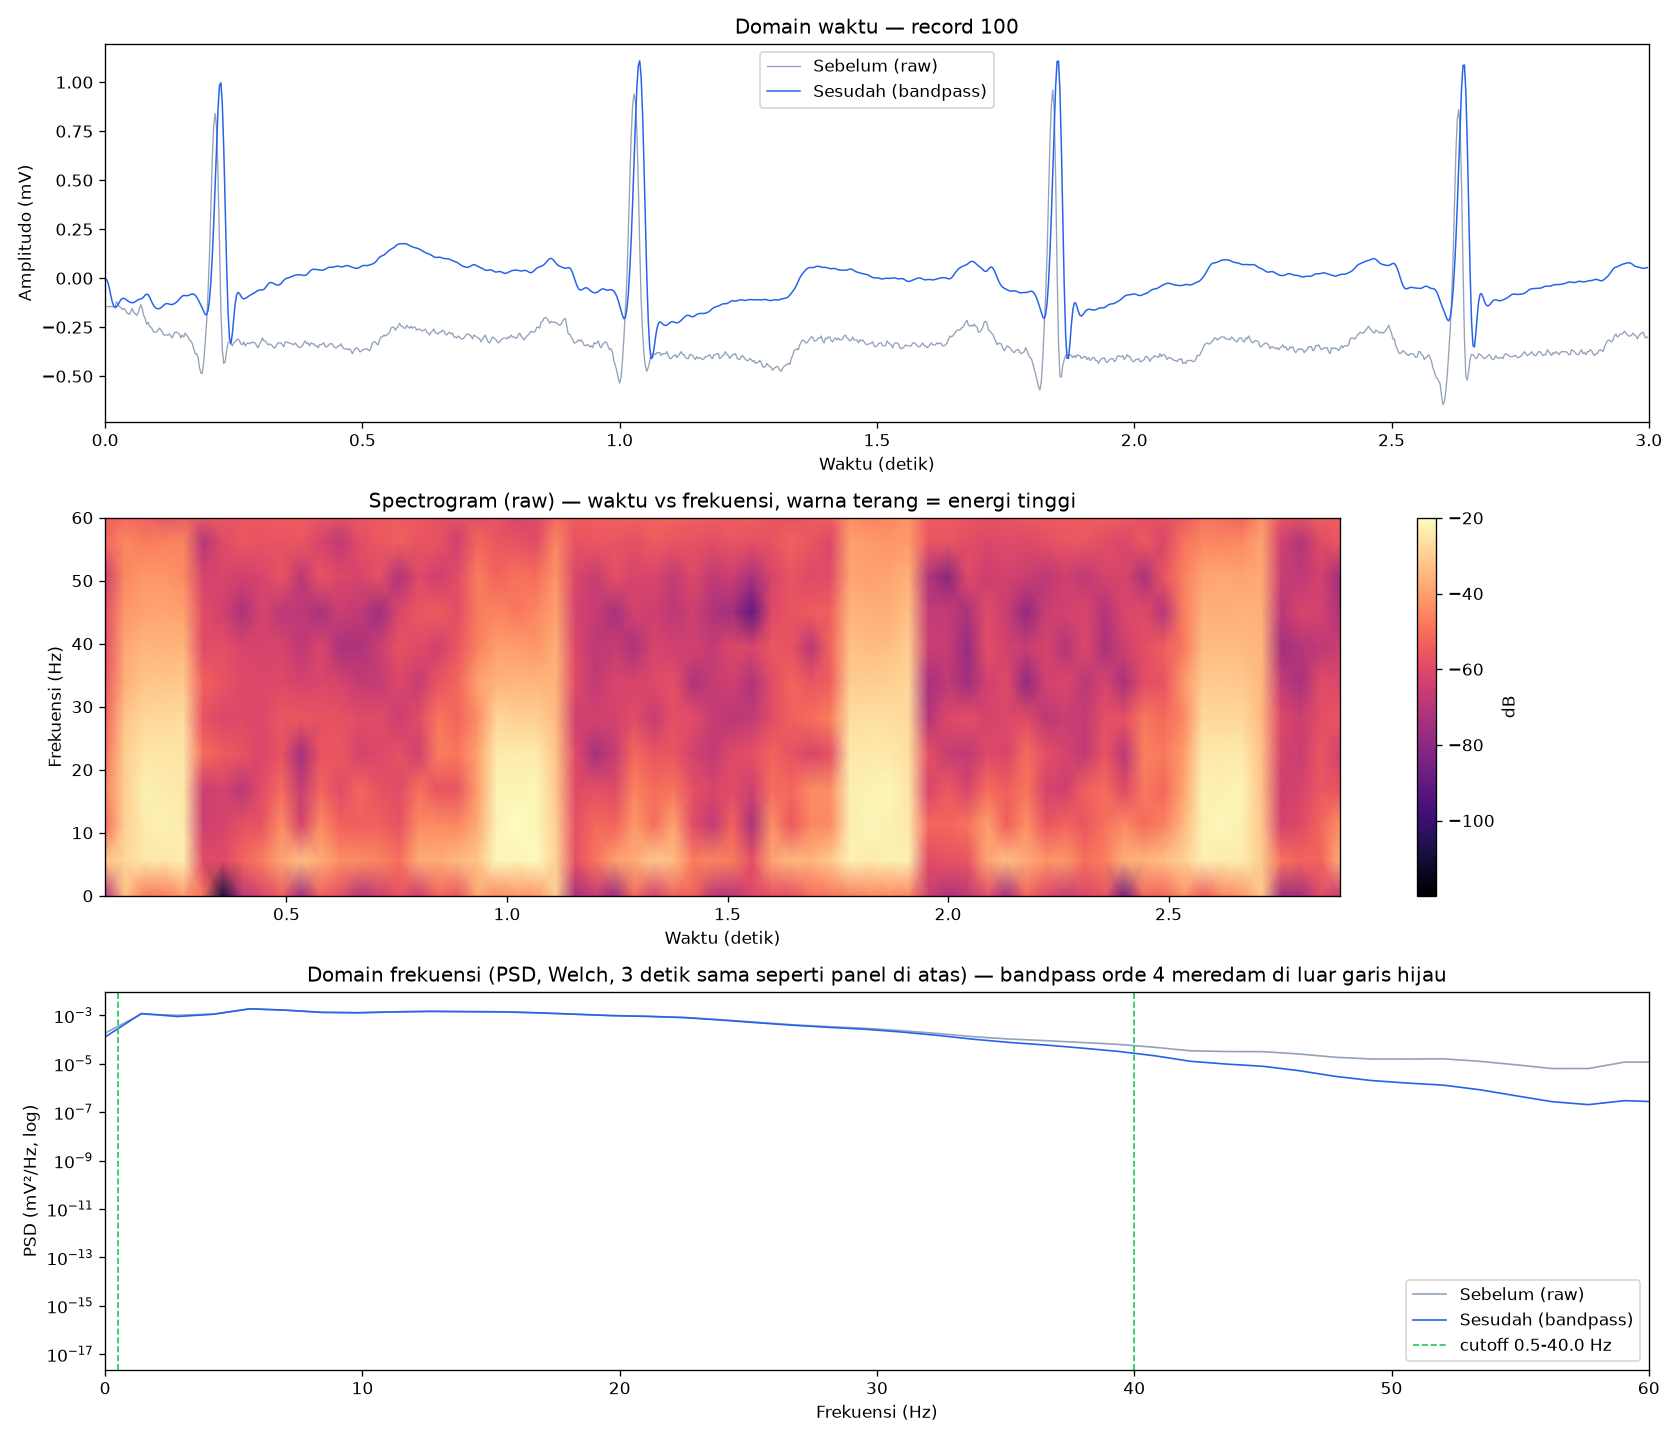
\includegraphics[width=\linewidth,height=0.5\textheight,keepaspectratio]{fase1_100.png}
  \caption{Sinyal rekaman 100 sebelum dan sesudah filter \textit{bandpass} kausal}
  \label{fig:hasil-filter}
\end{figure}

Gambar~\ref{fig:hasil-filter} terdiri atas tiga panel. Pada panel atas, filter memusatkan sinyal di sekitar nol, yaitu rata-rata berubah dari $-0{,}3063$ mV menjadi 0,0000 mV, sedangkan gelombang P, kompleks QRS, dan gelombang T tetap utuh. Simpangan baku sinyal hanya turun dari 0,1932 mV menjadi 0,1840 mV atau sekitar 4,8\%. Filter karena itu berperan sebagai pembersih dan bukan pemangkas morfologi. Puncak R pada sinyal tersaring tampak sedikit di kanan puncak pada sinyal mentah, yaitu \textit{group delay} sebesar 4 sampel atau sekitar 11 ms yang sengaja tidak dikoreksi. Panel tengah memperlihatkan spektrogram sinyal mentah dengan energi tertinggi mengumpul pada saat kompleks QRS dan pada frekuensi rendah. Pada panel bawah, kurva kerapatan spektral daya sesudah filter berimpit dengan kurva sebelum filter pada frekuensi rendah, lalu terpisah menjelang 40 Hz dan semakin jauh di bawahnya hingga 60 Hz.
% sumber: gambar laporan/buku-pa/gambar/fase1_100.png (dibuka dan dibaca); perhitungan ulang rekaman 100 (mean -0,3063 -> 0,0000, std 0,1932 -> 0,1840 = -4,8%); model/src/preprocessing.py design_bandpass_sos() (matriks 4 x 6, empat biquad); model/CLAUDE.md Fase 1 dan jebakan "Group delay filter kausal" (4 sampel / 360 Hz = 11,1 ms)

Hasil segmentasi \textit{window} 256 sampel beserta normalisasi \textit{z-score}, yang rancangannya ditunjukkan pada Gambar~\ref{fig:segmentasi}, diperiksa secara numerik pada rekaman 100. Sebanyak 2.273 anotasi menghasilkan 2.271 \textit{window} karena dua detak di tepi rekaman tidak memiliki cukup sampel. Setiap \textit{window} membentang 128 sampel atau sekitar 0,36 detik pada tiap sisi anotasi, dan seluruhnya berukuran 256 sampel dengan rata-rata mendekati nol serta simpangan baku 1,0000 setelah \textit{z-score}. Median indeks puncak R adalah 132 dan seluruh 2.271 \textit{window} memiliki puncak (nilai mutlak terbesar) dalam $\pm$2 sampel dari indeks tersebut.
% sumber: perhitungan ulang rekaman 100 dengan model/src/preprocessing.py segment_beats dan zscore_per_window (2.271 window, bentuk (2271, 256), median indeks puncak 132,0, seluruhnya dalam 132 +- 2, std z-score 1,0000); model/config.py (WIN_PRE 128, FS 360, 128/360 = 0,36 detik)

Ketiga tahap dinilai berjalan sesuai rancangan. Verifikasi ini hanya mencakup rekaman 100 dan 114. Pada rekaman 114, simpangan baku turun dari 0,3755 mV menjadi 0,3480 mV (7,3\%), seluruh 1.879 anotasi menghasilkan \textit{window}, dan 99,8\% \textit{window} memiliki puncak R dalam $\pm$2 sampel dari indeks 132.
% sumber: perhitungan ulang rekaman 114 (std 0,3755 -> 0,3480 = -7,3%, 1.879 window dengan 0 dibuang, 99,8% dalam 132 +- 2); model/CLAUDE.md Fase 1 (std 114 0,3755 -> 0,3480)

\subsubsection{Alur Hidup dan Beban Komputasi}

Seluruh rantai preprocessing harus berjalan secara \textit{real-time} di ESP32-S3 tanpa kehilangan sampel. Syaratnya adalah beban rata-rata per sampel lebih kecil daripada 2.778 $\mu$s atau 1/360 detik dan jumlah sampel yang hilang nol. Pengukuran memutar ulang sinyal acuan sampel demi sampel seolah-olah datang dari ADC pada 360 Hz, sedangkan waktu setiap panggilan pemrosesan dicatat dengan penghitung mikrodetik perangkat. Alur hidup yang diuji dimulai dari \textit{timer interrupt} atau \textit{interrupt service routine} (ISR) 360 Hz yang menaruh setiap sampel ke antrean 256 sampel. \textit{Loop} utama lalu menguras antrean dan memprosesnya sampai inferensi per detak, sebagaimana ditunjukkan pada Gambar~\ref{fig:alir-preprocessing}.
% sumber: firmware/test/test_inference/test_inference.cpp test_alur_hidup (anggaran 2778 us, micros(), golden_raw diputar per sampel); model/CLAUDE.md HW-3; firmware/src/akuisisi.cpp on_timer() dan loop(); firmware/include/ecg_live.h (ECG_LIVE_RING 4 * ECG_FS, ECG_LIVE_TIAP ECG_FS); model/docs/firmware-walkthrough.md bagian 5c

Hasil pengukuran ditunjukkan pada Tabel~\ref{tab:beban-komputasi}.

\begin{table}[!ht]
  \centering
  \caption{Beban komputasi dan antrean pada alur hidup}
  \label{tab:beban-komputasi}
  \setstretch{1.0}
  \setlength{\tabcolsep}{4pt}
  \renewcommand{\arraystretch}{1.15}
  \small
  \begin{tabularx}{\linewidth}{>{\RaggedRight\arraybackslash}X>{\raggedleft\arraybackslash}p{1.6cm}>{\RaggedRight\arraybackslash}X}
    \toprule
    \textbf{Besaran} & \textbf{Nilai} & \textbf{Kondisi Pengukuran} \\
    \midrule
    Anggaran waktu per sampel ($\mu$s) & 2.778 & 1/360 detik \\
    Beban rata-rata per sampel ($\mu$s) & 82 & \textit{Replay} sinyal acuan 2.400 sampel di perangkat, model \textit{window} 250 \\
    Puncak beban sesaat (ms) & 33,4 & Deteksi R-\textit{peak} dan inferensi bersamaan, model \textit{window} 250 \\
    Kapasitas antrean minimum menurut perhitungan (sampel) & 13 & Dihitung dari puncak beban sesaat \\
    Antrean saat puncak beban (sampel) & 12 & \textit{Firmware} produksi tanpa elektroda, ADC membaca derau, model \textit{window} 250 \\
    Antrean puncak (sampel) & 21 & \textit{Firmware} produksi dengan \textit{replay} sinyal acuan, model \textit{window} 256 \\
    Kapasitas antrean (sampel) & 256 & Antrean ISR pada kedua \textit{firmware} produksi \\
    Sampel hilang & 0 & Kedua pengukuran \textit{firmware} produksi \\
    \bottomrule
  \end{tabularx}
  \par\vspace{2pt}{\footnotesize\raggedright Keterangan: beban rata-rata setara 3,0\% anggaran dan puncak beban sesaat sekitar 12 kali anggaran. ISR adalah \textit{interrupt service routine}.\par}
\end{table}
% sumber: model/CLAUDE.md HW-3 (82 us/sampel dari 2778 us = 3,0%, burst 33,4 ms, antrean min 13), HW-4 (antrean 12 saat burst, sampel hilang 0), HW-7 Replay (antrean puncak 21/256, sampel hilang 0); model/docs/firmware-walkthrough.md bagian 5b dan 5c (burst 33.428 us, 12x anggaran satu sampel); 1/360 s = 2.777,8 us

Jalur preprocessing di perangkat tidak kehilangan sampel walaupun beban sesaatnya melampaui anggaran waktu (Tabel~\ref{tab:beban-komputasi}). Secara rata-rata pemrosesan hanya memakai 3,0\% anggaran per sampel. Beban itu menumpuk ketika deteksi R-\textit{peak} atas bufer empat detik bertepatan dengan inferensi detak baru, dan satu sampel dapat memakan sekitar 12 kali anggaran. Tanpa pembacaan ADC di ISR, setiap lonjakan seperti ini akan membuang sekitar 12 sampel dan merusak interval R-R. Antrean ISR menyerap lonjakan tersebut dengan terisi 12 sampel, mendekati kebutuhan 13 sampel hasil perhitungan dan jauh di bawah kapasitas 256 sampel atau sekitar 0,71 detik. Keluaran perangkat juga stabil, yaitu 11 detak per putaran \textit{replay} 6,67 detik atau sekitar 1,6 detak per detik, dengan pola probabilitas yang identik pada setiap putaran.
% sumber: model/CLAUDE.md HW-3, HW-4, HW-7 Replay (11 beat per putaran 6,67 detik, 11 / 6,67 = 1,65 beat/detik, pola p identik tiap putaran); model/CLAUDE.md jebakan "Beban alur hidup bursty" dan "Menunggu jaringan di dalam loop" (antrean 256 sampel @360 Hz = 711 ms); 256 / 360 = 0,711 detik

Pada pengujian \textit{replay} ditemukan satu kegagalan yang tidak langsung terlihat. Konversi nilai sinyal acuan dari \textit{float} ke \textit{count} ADC di dalam ISR membuat \textit{board} mengalami \textit{panic} bertipe \textit{coprocessor exception} pada detik ke-18,49, jadi lolos pada uji singkat. Penyebabnya, ESP32 tidak menyimpan register FPU saat masuk ISR. Penanganannya adalah mengonversi seluruh sinyal acuan ke tabel bilangan bulat sekali di \textit{setup}, dengan tambahan pemakaian RAM dari 21,2\% menjadi 22,7\% untuk tabel sebesar 4.800 byte. \textit{Board} yang me-\textit{reset} diam-diam membuat \textit{replay} nonaktif dan pengukuran melaporkan derau ADC. Status \textit{replay} karena itu diverifikasi dari ayunan sinyal.
% sumber: model/CLAUDE.md jebakan "Float di dalam ISR membunuh ESP32" (EXCCAUSE 0x00000004, detik 18, sim_counts); model/docs/firmware-walkthrough.md (panic di detik 18,49, RAM 21,2% -> 22,7%, sim_counts 4.800 byte); firmware/src/akuisisi.cpp (sim_counts dan on_timer)

Alur hidup dinilai memenuhi syarat \textit{real-time} pada sinyal \textit{replay}, yaitu beban rata-rata jauh di bawah anggaran dan sampel hilang nol. Beban rata-rata 82 $\mu$s dan puncak 33,4 ms diukur pada versi model \textit{window} 250 dan belum diukur ulang pada \textit{window} 256. Antrean puncak pada \textit{window} 256 tercatat 21 sampel, lebih tinggi daripada 12 sampel pada versi lama dan setara dengan sekitar 58 ms sampel yang tertahan. Kenaikan ini tidak dapat dijelaskan oleh pertambahan waktu inferensi per detak dari 26,0 ms menjadi 26,6 ms dan penyebabnya belum ditelusuri. Meskipun demikian, 21 sampel baru sekitar 8\% kapasitas antrean 256 sampel dan sampel hilang tetap nol. Pengukuran ini belum mencakup sinyal tubuh dan belum mencakup beban saat WiFi dan MQTT aktif.
% sumber: model/CLAUDE.md HW-1 (26,6 ms per detak, dari 26,0), HW-3 (versi window 250), HW-4 (antrean 12 saat burst), HW-7 Replay (antrean puncak 21/256 pada window 256, sampel hilang 0); 21 / 360 = 0,0583 detik = 58 ms; 21 / 256 = 8,2%

\subsubsection{Uji Perangkat dan Integrasi di \textit{Board}}

Setiap komponen perangkat diuji fungsinya, dan jalur \textit{real-time} diperiksa tetap tidak kehilangan sampel ketika layar dan \textit{buzzer} ikut bekerja, mengikuti rencana pengujian perangkat keras. Seluruh rangkaian uji di \textit{board} dijalankan pada 13 Oktober 2026 dengan rangkaian berpeta pin PCB, dan hasilnya per rangkaian uji ditunjukkan pada Tabel~\ref{tab:uji-papan}.
% sumber: git log f6042b5 (2026-10-13, "board 29/29, native 23/23") dan 07a5a07 (2026-10-13, "board: 29/29 test perangkat, native 23/23"); firmware/README.md bagian Test (jumlah per suite)

\begin{table}[!ht]
  \centering
  \caption{Hasil rangkaian uji di ESP32-S3 pada 13 Oktober 2026}
  \label{tab:uji-papan}
  \setstretch{1.0}
  \setlength{\tabcolsep}{4pt}
  \renewcommand{\arraystretch}{1.15}
  \small
  \begin{tabular}{>{\RaggedRight\arraybackslash}p{3.0cm}>{\centering\arraybackslash}p{1.5cm}>{\RaggedRight\arraybackslash}p{6.6cm}>{\centering\arraybackslash}p{1.4cm}}
    \toprule
    \textbf{Rangkaian Uji} & \textbf{Kasus} & \textbf{Yang Diverifikasi} & \textbf{Hasil} \\
    \midrule
    Inferensi & 5 & Inferensi model INT8 di perangkat, latensi, dan \textit{tensor arena} & Lulus \\
    Integrasi & 5 & Jalur \textit{real-time} utuh dengan layar dan \textit{buzzer} aktif; sampel hilang 0, laju jantung dalam 3 bpm & Lulus \\
    Layar & 2 & Inisialisasi TFT dan transfer SPI satu layar penuh & Lulus \\
    ADC dan \textit{lead-off} & 2 & ADC terbaca dan pewaktu menghasilkan 360 sampel per detik & Lulus \\
    Tombol & 2 & Ketiga pin berlogika HIGH saat diam dan uji tombol berakhir tepat pada batas waktunya & Lulus \\
    \textit{Buzzer} & 1 & Pin tersambung ke pembangkit nada setelah SPI layar terpasang, diam pada logika HIGH & Lulus \\
    Jumlah & 17 & & 17 lulus \\
    \bottomrule
  \end{tabular}
\end{table}
% sumber: firmware/README.md tabel Test dan baris "board 29 (test_preproc 11, test_inference 5, test_hw_integrasi 5, test_hw_tft 2, test_hw_adc 2, test_hw_tombol 2, test_hw_buzzer 1, test_hw_ina219 1)"; jumlah RUN_TEST per suite di firmware/test/test_*/; firmware/test/test_hw_integrasi/ (n_lewat == 0, PUTARAN 3, HR beda <= 3 bpm, label sama PC); git log f6042b5 (board 29/29)

Seluruh 17 kasus pada Tabel~\ref{tab:uji-papan} lulus. Hasil terpenting adalah uji integrasi. Pengukuran beban pada Tabel~\ref{tab:beban-komputasi} belum mencakup layar dan \textit{buzzer}, sedangkan uji integrasi menunjukkan sampel hilang tetap nol ketika gelombang digambar dan bip dibunyikan selama tiga putaran sinyal acuan. Uji integrasi juga memeriksa laju jantung yang ditampilkan, yaitu berselisih paling banyak 3 bpm dari interval R-R anotasi. Cakupannya perlu dicatat. Uji otomatis tidak menilai bunyi \textit{buzzer}, warna layar, dan tekanan tombol sungguhan, karena hal tersebut memerlukan pengamatan manusia dan diperiksa melalui menu Tes perangkat yang hasilnya tidak dicatat sebagai berkas. Uji integrasi juga dijalankan tanpa WiFi dan MQTT, jadi beban radio pada jalur \textit{real-time} belum tercakup dalam hasil ini.

Penguncian sesi perekaman diuji terpisah dengan menyuntikkan tekanan tombol dan perintah melalui serial ke perangkat yang sedang berjalan. Tujuh skenario diuji, yaitu sebagai berikut.
\begin{enumerate}
  \item Menu terkunci saat merekam.
  \item Menu tetap terkunci saat dijeda.
  \item Perubahan sumber, mode daya, pelewatan kalibrasi, WiFi, dan \textit{broker} ditolak saat merekam.
  \item Perekaman ditolak saat sumber \textit{replay}.
  \item Perekaman ditolak saat menu terbuka.
  \item Jeda dan lanjut diakhiri penyimpanan.
  \item Menu dapat dibuka kembali sesudah rekaman disimpan.
\end{enumerate}
Ketujuh skenario lulus pada dua putaran dengan sampel hilang nol selama sesi perekaman.
% sumber: git log 5088bb6 (2026-10-13, kunci sesi rekam: uji_alur_rekam.py 7/7 LULUS 2 putaran, sampel hilang 0 selama sesi rekam, pio test esp32-s3 29/29, native 23/23); model/scripts/uji_alur_rekam.py (skenario a-g, tombol disuntik lewat serial t/T); git log f6042b5 (native 23/23); firmware/test/test_hw_integrasi/ (PUTARAN 3, TFT digambar dan buzzer dibunyikan di loop uji, tanpa WiFi); firmware/README.md ("Bunyi buzzer dan isi layar dinilai langsung", menu Tes perangkat); bab4 tab:beban-komputasi (diukur tanpa antarmuka)

\subsubsection{Segmentasi di Perangkat}

Di perangkat, posisi R-\textit{peak} berasal dari detektor Pan-Tompkins, bukan dari anotasi seperti pada pelatihan. Biaya perbedaan itu diukur sebagai jumlah detak yang terlewat dan besarnya pengaruh pada klasifikasi. Pengukuran memakai DS2 dengan rangkaian koreksi posisi yang sama dengan kode C, yaitu kompensasi 38 sampel, penyelarasan ke puncak sinyal dalam $\pm$25 sampel, dan pengurangan \textit{group delay} 4 sampel. Nilai 38 sampel adalah median selisih antara deteksi dan anotasi pada DS1 dengan simpangan baku 13 sampel, jadi DS2 hanya dipakai untuk mengukur dan tidak untuk memilih parameter. Angka klasifikasi diukur pada model akhir versi \textit{float32}, yaitu \textit{window} 256 sampel dan \textit{threshold} 0,80, dan pada model acuan berukuran \textit{window} 250 sampel dengan \textit{threshold} 0,35 sebagai pembanding. Angka \textit{sensitivity} detektor tidak melibatkan model.
% sumber: model/docs/segmentasi-deteksi-walkthrough.md §1 dan §3 (offset median 38 sampel dikalibrasi di DS1; dua model: baseline window 90/160 threshold 0,35 dan model berlaku window 128/128 threshold 0,80, diukur ulang 13 Okt 2026 dengan model/scripts/eval_detected_segmentation.py); model/CLAUDE.md decision "Segmentasi on-device" (std 13 sampel); firmware/include/ecg_preproc.h (ECG_PT_OFFSET 38, ECG_PT_REFINE 25, ECG_GROUP_DELAY 4)

Keluaran detektor jatuh di sebelah kanan anotasi pasangannya, yaitu pada garis dasar sesudah kompleks QRS dan bukan pada puncak R. Pada sepuluh detik pertama rekaman 100, seluruh 13 anotasi memiliki 13 deteksi pasangan tanpa deteksi yang terlewat maupun berlebih. Pada keseluruhan rekaman 100, median selisih posisi adalah 40 sampel atau sekitar 0,11 detik, sejalan dengan median 38 sampel dari DS1. Keterlambatan ini sistematis dan karena itu dapat dikompensasi dengan satu konstanta, sedangkan penyelarasan ke puncak sinyal menyerap sisa variasinya.
% sumber: perhitungan ulang rekaman 100 dengan model/src/preprocessing.py pan_tompkins_detect (13 anotasi dan 13 deteksi pada 10 detik pertama, median selisih 40 sampel, std 12,1 sampel, 99,9% dalam 38 +- 25; 40/360 = 0,11 detik)

Detektor tidak melewatkan detak dengan peluang yang sama pada semua kelas, sebagaimana ditunjukkan pada Tabel~\ref{tab:sensitivity-detektor}.

\begin{table}[!ht]
  \centering
  \caption{\textit{Sensitivity} detektor Pan-Tompkins per kelas AAMI pada DS2}
  \label{tab:sensitivity-detektor}
  \setstretch{1.0}
  \setlength{\tabcolsep}{4pt}
  \renewcommand{\arraystretch}{1.15}
  \small
  \begin{tabular}{>{\RaggedRight\arraybackslash}p{4.2cm}>{\RaggedRight\arraybackslash}p{4.6cm}>{\centering\arraybackslash}p{3.0cm}}
    \toprule
    \textbf{Kelas} & \textbf{Keterangan} & \textbf{\textit{Sensitivity}} \\
    \midrule
    N & Normal & 0,9614 \\
    S & Supraventrikular, datang prematur & 0,6494 \\
    V & Ventrikular & 0,9146 \\
    F & Fusi & 0,9820 \\
    S, V, F, dan Q gabungan & Seluruh aritmia & 0,8296 \\
    Seluruh detak & 47.074 terdeteksi dan 2.638 terlewat & 0,9469 \\
    \bottomrule
  \end{tabular}
  \par\vspace{2pt}{\footnotesize\raggedright Keterangan: deteksi dipasangkan dengan anotasi dalam jendela 150 ms. Detektor juga menghasilkan 2.194 deteksi tanpa pasangan anotasi, jadi \textit{positive predictivity} seluruh detak 0,9555.\par}
\end{table}
% sumber: model/src/evaluate.py pair_detected dan model/scripts/eval_detected_segmentation.py (TOLERANSI_MS = 150); model/docs/segmentasi-deteksi-walkthrough.md bagian 3 (2.194 deteksi palsu); 47.074 / (47.074 + 2.194) = 0,9555; QRS Se dan +P dengan jendela 150 ms mengikuti PhysioNet bxb (docs/2026-11-01-crosscheck-metrik-bab4/klasifikasi.md butir 12)
% sumber: model/docs/segmentasi-deteksi-walkthrough.md bagian 3 dan 4 (47.074 terdeteksi, 2.638 terlewat, sensitivity 0,9469; per kelas N 0,9614, S 0,6494, V 0,9146, F 0,9820, Normal vs Aritmia 0,9614 vs 0,8296); model/scripts/eval_detected_segmentation.py (aritmia = S V F Q); diukur dengan detektor yang sama sebelum window dikunci 256, perhitungannya hanya dari pasangan deteksi dan anotasi sehingga tidak melibatkan model

Detektor menemukan 96,14\% detak Normal tetapi hanya 82,96\% detak aritmia (Tabel~\ref{tab:sensitivity-detektor}), dan kelas S menjadi yang paling sering terlewat dengan \textit{sensitivity} 0,6494. Penjelasan yang paling sesuai bersifat struktural. Detak supraventrikular datang prematur, sedangkan Pan-Tompkins menutup deteksi selama periode refraktori 200~ms sesudah detak sebelumnya, jadi detak yang datang terlalu cepat berpeluang terblokir. Penjelasan ini belum diuji dengan mengubah periode refraktori.
% sumber: model/docs/segmentasi-deteksi-walkthrough.md §4 (sebab struktural: beat S prematur terblokir periode refraktori 200 ms, PT_REFRACTORY_MS di model/config.py; trade-off refraktori belum diukur)

Dampak segmentasi hasil detektor terhadap klasifikasi ditunjukkan pada Tabel~\ref{tab:segmentasi-deteksi}. \textit{Recall} sistem memakai penyebut seluruh detak aritmia asli, termasuk yang tidak pernah terdeteksi, sedangkan \textit{recall}, \textit{precision}, dan F1 lainnya dihitung pada detak yang terdeteksi.

\begin{table}[!ht]
  \centering
  \caption{Klasifikasi DS2 model \textit{float32} dengan segmentasi anotasi dan segmentasi hasil detektor}
  \label{tab:segmentasi-deteksi}
  \setstretch{1.0}
  \setlength{\tabcolsep}{4pt}
  \renewcommand{\arraystretch}{1.15}
  \small
  \begin{tabular}{>{\RaggedRight\arraybackslash}p{3.0cm}>{\centering\arraybackslash}p{2.2cm}>{\centering\arraybackslash}p{2.2cm}>{\centering\arraybackslash}p{2.2cm}>{\centering\arraybackslash}p{2.2cm}}
    \toprule
    \textbf{Metrik} & \textbf{Acuan, anotasi} & \textbf{Acuan, detektor} & \textbf{Akhir, anotasi} & \textbf{Akhir, detektor} \\
    \midrule
    \textit{Recall} & 0,6661 & 0,6821 & 0,6996 & 0,7279 \\
    \textit{Precision} & 0,4919 & 0,4794 & 0,6235 & 0,5869 \\
    F1 & 0,5659 & 0,5631 & 0,6594 & 0,6499 \\
    \textit{Recall} sistem & 0,6661 & 0,5656 & 0,6996 & 0,6035 \\
    \bottomrule
  \end{tabular}
\end{table}
% sumber: model/docs/segmentasi-deteksi-walkthrough.md §3 tabel A (recall, precision, F1 baseline anotasi/deteksi dan berlaku anotasi/deteksi) dan blok B (recall sistem: baseline 3.084 / 5.453 = 0,5656, berlaku 3.291 / 5.453 = 0,6035); model/artifacts/metrics/fase6b_segmentasi_deteksi.csv memuat baris model acuan (f1 0,565903 / 0,563082, recall_sistem 0,666055 / 0,565560)

Segmentasi di perangkat tidak merusak klasifikasi selama ketiga koreksi posisi diterapkan (Tabel~\ref{tab:segmentasi-deteksi}). F1 dengan segmentasi detektor berselisih kurang dari 0,01 dari F1 dengan segmentasi anotasi pada kedua model, yaitu 0,6499 dibandingkan 0,6594 pada model akhir \textit{float32}. \textit{Recall} sistem model akhir turun dari 0,6996 menjadi 0,6035, dan seluruh penurunan ini berasal dari detak yang tidak pernah sampai ke model.

Penurunan \textit{recall} sistem tersebut berarti hanya 3.291 dari 5.453 detak aritmia asli yang tertangkap detektor lalu dikenali model. Detektor juga menghasilkan 2.194 deteksi palsu, dan 50,4\% di antaranya diklasifikasi Aritmia oleh model akhir, menambah 1.106 alarm palsu.
% sumber: model/docs/segmentasi-deteksi-walkthrough.md §3 blok B dan C (berlaku: 3.291 dari 5.453 tertangkap; 2.194 deteksi palsu, 50,4% diklasifikasi Aritmia = 1.106 alarm palsu tambahan); 0,6996 - 0,6035 = 0,0961

Segmentasi di perangkat dengan demikian layak, dan biayanya terletak pada detektor, bukan pada model. Detektor melewatkan sekitar 5\% detak secara keseluruhan dan sekitar sepertiga detak kelas S, sedangkan klasifikasi pada detak yang terdeteksi setara dengan klasifikasi pada segmentasi anotasi. Ketergantungan model terhadap posisi R yang presisi ditangani dengan latihan ber-\textit{jitter} pada jalur model.
% sumber: tab:sensitivity-detektor (sensitivity seluruh detak 0,9469, S 0,6494), tab:segmentasi-deteksi; model/docs/jitter-walkthrough.md (latih ulang dengan jitter)

\subsubsection{Akuisisi Sinyal Tubuh}

Sinyal tubuh dari modul AD8232 dinilai kelayakannya sebagai masukan jalur preprocessing. Rekaman diambil dengan konfigurasi Lead II, elektroda \textit{wet-gel}, dan daya dari \textit{powerbank} agar perangkat tidak tersambung ke jala-jala selama perekaman. Setiap rekaman dilaporkan dengan empat ukuran, yaitu ayunan sinyal ADC absolut, persentase dengung 50 Hz terhadap energi pita ECG 0,5--40 Hz~\cite{gajdzik_2026}, jumlah R-\textit{peak} yang ditemukan Pan-Tompkins, dan jumlah sampel jenuh. Kelayakan rekaman dinilai dengan indeks kualitas sinyal per jendela 10 detik. Pada rekaman yang dijeda, R-\textit{peak} dan interval R-R dihitung per segmen agar tidak ada interval R-R yang melintasi jeda.

Ayunan dalam mV dihitung sebagai ekuivalen masukan AD8232, yaitu jumlah \textit{count} dikalikan 0,757 mV per \textit{count} dari ADC 12-bit dengan atenuasi 11 dB, lalu dibagi \textit{gain} AD8232 sekitar 1.100. Dengan konversi ini, ECG sehat berayun sekitar 2 mV atau sekitar 3.000 \textit{count}, sedangkan ayunan di bawah sekitar 0,1 mV atau 150 \textit{count} berarti tidak ada biopotensial sama sekali.

Ayunan, dengung, dan sampel jenuh dilaporkan tanpa ambang lulus, karena acuan baku untuk ambang ketiganya tidak ditemukan. Definisi rasio dengung mengikuti penelitian yang membandingkan jalur akuisisi AD8232 dengan ADC 12-bit ESP32, yang juga tidak menetapkan ambang lulus~\cite{gajdzik_2026}. Sampel jenuh adalah sampel di batas atas atau bawah ADC. Gerbang kualitas waktu nyata, yaitu kontak elektroda dan interval R-R, dipakai sebelum detak diteruskan dan diuji tersendiri dengan sinyal tubuh.
% sumber: model/CLAUDE.md jebakan "Telemetri akuisisi bisa berbohong" (konversi 12-bit + atten 11 dB = 0,757 mV/count, gain AD8232 sekitar 1100, EKG sehat sekitar 2 mV sekitar 3000 count, di bawah sekitar 0,1 mV sekitar 150 count tidak ada biopotensial); model/docs/akuisisi-walkthrough.md bagian 1 (USB laptop vs power bank) dan bagian 6 (ukuran dan ambang); firmware/src/perangkat.cpp (ADC_WIDTH_BIT_12, ADC_ATTEN_DB_12, nama lain atenuasi 11 dB); model/scripts/analyze_recording.py (masuk_akal 30-200 bpm; muat() dan analisis_segmen() memisah segmen pada baris jeda)
% sumber: keputusan user 1 Nov 2026 (ambang tanpa rujukan dihapus: dengung < 15%, autokorelasi > 0,25, BPM wajar > 90%, jenuh 0,1%, status Berhasil/Bersinyal/Gagal; diganti indeks kualitas per jendela 10 detik); Gajdzik dkk. 2026 hlm. 59-63 (PLIratio tanpa ambang lulus); rail jenuh ADC_ATAS 4090 dan ADC_BAWAH 5 dari model/scripts/analyze_recording.py hitung_clipping(); gerbang waktu nyata dari bab3.tex gerbang kualitas

Kelayakan setiap rekaman dinilai per jendela 10 detik dengan indeks kualitas sinyal empat langkah~\cite{syversen_2024}, jadi bagian rekaman yang buruk tidak tersembunyi oleh nilai keseluruhan. Tiga langkah pertama memeriksa kelayakan fisiologis, yaitu detak per menit 40 sampai 180, jeda antar-R-\textit{peak} paling lama 3 detik, dan rasio interval R-R terpanjang terhadap terpendek di bawah 2,2. Langkah keempat memotong setiap kompleks QRS selebar median interval R-R dan merata-ratakannya menjadi \textit{template}. Jendela dinyatakan lolos bila rerata korelasi setiap potongan terhadap \textit{template} minimal 0,66. Hasil pengujian rekaman resmi ditunjukkan pada Tabel~\ref{tab:kualitas-rekaman}.
% sumber: Syversen dkk. 2024 bagian SQI1 ("HR-check of 40 and <180 bpm, ... maximum space between subsequent R-peaks is <3 s ... ratio is <2.2 ... adaptive template matching threshold (0.66)"), metode asli Orphanidou dkk. 2015 hlm. 834-836 (potongan selebar median RR berpusat di R); model/scripts/kualitas_jendela.py; model/docs/akuisisi-walkthrough.md bagian 6 SQI per jendela 10 detik

\begin{table}[!ht]
  \centering
  \caption{Kualitas rekaman AD8232 pada pengujian rekaman resmi}
  \label{tab:kualitas-rekaman}
  \setstretch{1.0}
  \setlength{\tabcolsep}{2.5pt}
  \renewcommand{\arraystretch}{1.15}
  \footnotesize
  \begin{tabular}{>{\centering\arraybackslash}p{1.5cm}>{\raggedleft\arraybackslash}p{1.1cm}>{\centering\arraybackslash}p{1.8cm}>{\raggedleft\arraybackslash}p{1.4cm}>{\raggedleft\arraybackslash}p{1.1cm}>{\raggedleft\arraybackslash}p{1.0cm}>{\raggedleft\arraybackslash}p{1.2cm}>{\raggedleft\arraybackslash}p{1.3cm}>{\raggedleft\arraybackslash}p{1.5cm}}
    \toprule
    \textbf{Rekaman} & \textbf{Durasi (detik)} & \textbf{Ayunan (\textit{count} / mV)} & \textbf{Dengung (\%)} & \textbf{R-\textit{peak}} & \textbf{Jenuh} & \textbf{Jendela} & \textbf{Jendela Lolos (\%)} & \textbf{Korelasi Mini\-mum} \\
    \midrule
    \multicolumn{9}{l}{\textit{Sesi 22 Oktober 2026, subjek S01, Lead II, catu powerbank}} \\
    R1 & 300,0 & 2.928 / 2,01 & 1,9 & 402 & 1 & 30 & 100,0 & 0,981 \\
    R2 & 300,0 & 3.012 / 2,07 & 3,1 & 408 & 5 & 30 & 100,0 & 0,967 \\
    R3 & 300,0 & 3.104 / 2,14 & 2,9 & 425 & 9 & 30 & 100,0 & 0,967 \\
    R4 & 27,1 & 2.919 / 2,01 & 3,8 & 40 & 1 & 2 & 100,0 & 0,980 \\
    \bottomrule
  \end{tabular}
  \par\vspace{2pt}{\footnotesize\raggedright Keterangan: R1 sampai R4 adalah empat rekaman berurutan dari satu sesi tanpa jeda. Jenuh adalah jumlah sampel di batas ADC, paling banyak 0,010\% sampel rekaman. Jendela adalah jumlah jendela 10 detik utuh. Korelasi minimum adalah rerata korelasi \textit{template} terendah di antara jendela rekaman. Status \textit{lead-off} 0\% pada keempat rekaman.\par}
\end{table}
% sumber: jendela, jendela lolos, dan korelasi minimum dari model/scripts/kualitas_jendela.py -> model/artifacts/metrics/kualitas/jendela10s_20261022-*.csv (30/30/30/2 jendela, 100% lolos, korelasi minimum 0,981, 0,967, 0,967, 0,980)
% sumber: keluaran make analisis FILE=data/recordings/<nama>.csv pada 20261022-1256-rekam-001 (ADC 1167..4095, dengung 1,9%, autokorelasi 0,37 median per 30 s, R-peak 402 dalam 300,0 detik, masuk akal 100%), -1256-rekam-002 (1083..4095, 3,1%, 0,38, 408), -1257-rekam-003 (991..4095, 2,9%, 0,33, 425), -1257-rekam-004 (1176..4095, 3,8%, 0,28 tanpa jendela, 40 dalam 27,1 detik); ayunan = maks - min (2.928, 3.012, 3.104, 2.919), mV = count x 0,757 / 1100 (2,01, 2,07, 2,14, 2,01); jenuh dengan rail firmware 4090/5 = 1, 5, 9, 1 sampel (0,001%, 0,005%, 0,008%, 0,010%); header lepas=0 (0%) pada keempat berkas; rekaman uji coba 10 Sep - 11 Okt 2026 tidak dimasukkan (arsip model/data/arsip/rekaman-uji-coba/, bukan hasil)

Keempat rekaman resmi lolos indeks kualitas sinyal pada seluruh jendela 10 detik (Tabel~\ref{tab:kualitas-rekaman}). Korelasi \textit{template} terendah 0,967, jauh di atas batas 0,66, dan ayunan sekitar 2 mV sesuai dengan ECG sehat. Dengung paling besar 3,8\%, dan sampel jenuh hanya muncul sesekali pada puncak R. Penilai yang sama menolak seluruh jendela rekaman uji coba yang hanya berisi derau, jadi kelolosan ini bukan akibat syarat yang terlalu longgar. Sinyal tubuh pada sesi ini karena itu layak dijadikan masukan jalur preprocessing.
% sumber: tab:kualitas-rekaman (92 jendela lolos 100%, korelasi minimum 0,967 pada R2 dan R3; dengung maksimum 3,8% pada R4; ayunan 2,01-2,14 mV; jenuh maksimum 1 dari 9.771 = 0,010%); kontrol negatif rekaman uji coba arsip berayun 16-55 count lolos 0% jendela (model/docs/akuisisi-walkthrough.md bagian 6)

Bentuk sinyal rekaman yang berhasil ditunjukkan pada Gambar~\ref{fig:rekaman-berhasil}, yaitu enam detik pertama rekaman R1.

\begin{figure}[!ht]
  \centering
  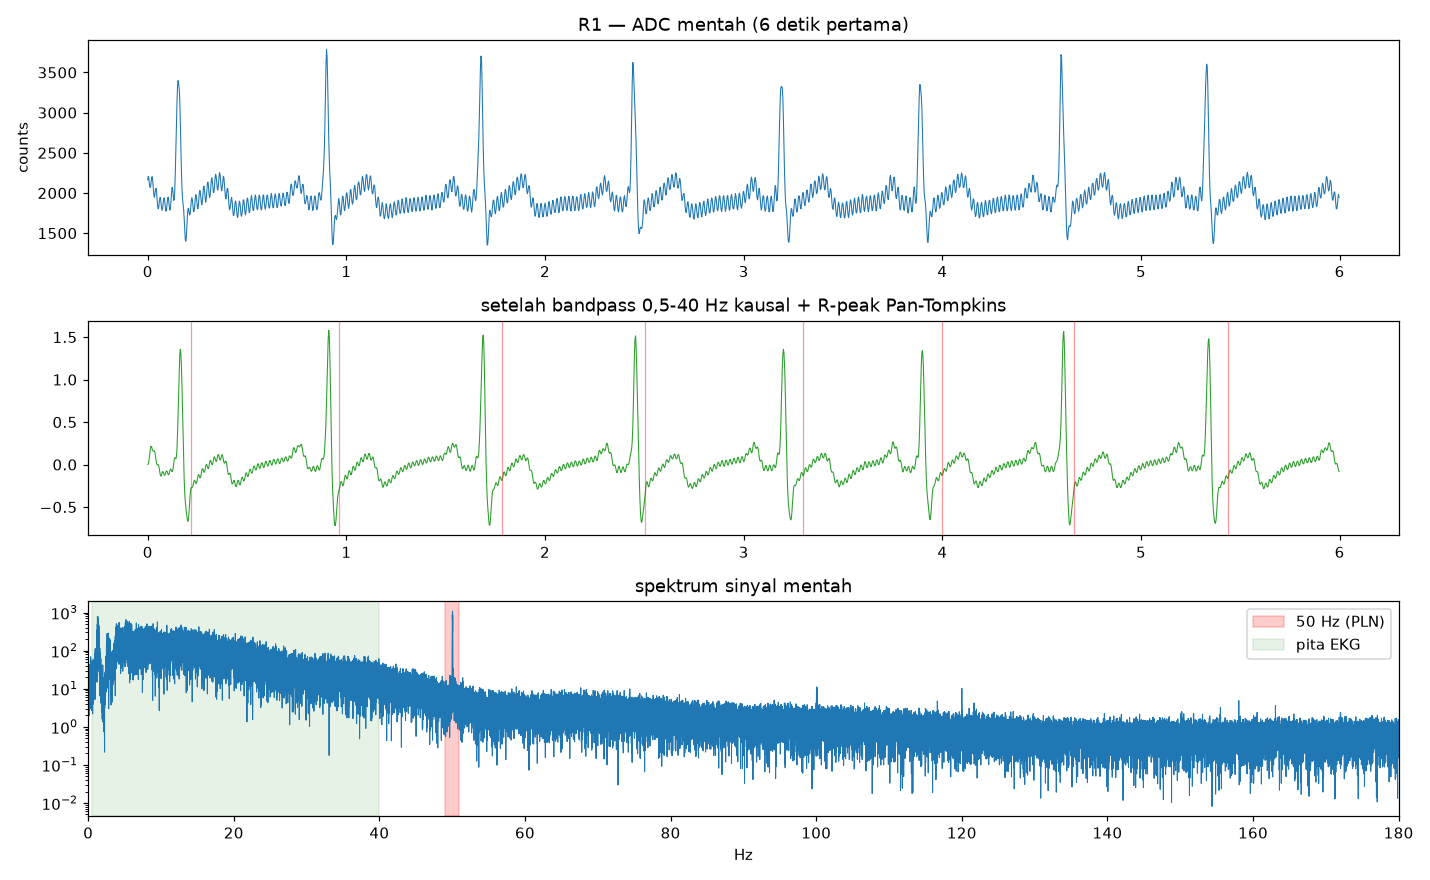
\includegraphics[width=\linewidth,height=0.45\textheight,keepaspectratio]{akuisisi_20261022-1256-rekam-001.png}
  \caption{Rekaman AD8232 yang berhasil, enam detik pertama rekaman R1}
  \label{fig:rekaman-berhasil}
\end{figure}
% sumber: model/artifacts/metrics/akuisisi/akuisisi_20261022-1256-rekam-001.png (make analisis), disalin ke laporan/buku-pa/gambar oleh scripts/export_artifacts.sh --laporan

Gambar~\ref{fig:rekaman-berhasil} terdiri atas tiga panel. Panel pertama menampilkan ADC mentah, dan panel kedua sinyal sesudah \textit{bandpass} dengan garis merah pada setiap R-\textit{peak} hasil Pan-Tompkins. Panel ketiga menampilkan spektrum dengan pita merah untuk dengung 50 Hz serta pita hijau untuk pita ECG. Pada panel pertama, puncak QRS mencapai sekitar 3.300 sampai 3.800 \textit{count} di atas garis dasar sekitar 1.900 \textit{count}. Panel kedua memuat delapan R-\textit{peak} dengan jarak antarpuncak sekitar 0,7 sampai 0,8 detik. Panel ketiga memperlihatkan puncak sempit pada 50 Hz di luar pita ECG. Filter \textit{bandpass} hanya meredam 50 Hz sebesar 9,3 dB, yaitu penguatan 0,342, jadi dengung yang masuk ke ADC tetap tampak sebagai gerigi halus pada garis dasar panel kedua.
% sumber: dibaca dari model/artifacts/metrics/akuisisi/akuisisi_20261022-1256-rekam-001.png (puncak QRS 3.300-3.800 count, garis dasar sekitar 1.900, 8 garis R-peak dalam 6 detik, puncak 50 Hz pada spektrum)
% sumber: tiga panel dari model/scripts/analyze_recording.py (ADC mentah, bandpass + garis R-peak, spektrum pita 50 Hz merah dan pita EKG hijau; model/docs/akuisisi-walkthrough.md §5); model/docs/akuisisi-walkthrough.md §2 (bandpass meredam 50 Hz -9,3 dB, gain 0,342) dan perhitungan ulang sosfreqz atas model/src/preprocessing.py design_bandpass_sos() pada 50 Hz (gain 0,3422 = -9,31 dB)

Prosedur perekaman pada pengujian ini, yaitu catu daya \textit{powerbank}, elektroda baru yang ditempel sekali, dan penilaian kualitas dari ayunan ADC absolut, disusun dari perekaman uji coba selama pengembangan. Perekaman uji coba tersebut memakai rangkaian yang masih berubah sehingga tidak dilaporkan sebagai hasil.
% sumber: model/docs/akuisisi-walkthrough.md §1 (powerbank, elektroda sekali tempel), §6 (ayunan ADC absolut sebagai wasit) dan §8 (rekaman uji coba, arsip model/data/arsip/rekaman-uji-coba/)

Keberadaan R-\textit{peak} tidak dapat dijadikan penentu kualitas sinyal. Pan-Tompkins tetap melaporkan R-\textit{peak} karena ambangnya adaptif terhadap sinyal yang ada, dan keadaan tanpa sinyal bukan kondisi yang dikenalinya. Pada \textit{firmware}, tanpa elektroda dan tanpa \textit{replay}, alat mengeluarkan sekitar 2 detak per detik dengan 57\% di antaranya diklasifikasi Aritmia. Kualitas sinyal di perangkat karena itu dinilai dari kontak elektroda, yaitu status \textit{lead-off}, ayunan ADC, dan dengung 50 Hz.
% sumber: model/CLAUDE.md jebakan "Tanpa elektroda, alat mengarang aritmia: ~2 beat/detik, 57% ARITMIA" dan "Telemetri akuisisi bisa berbohong"; model/docs/akuisisi-walkthrough.md bagian 6

Hasil akuisisi tersebut adalah status fungsional, bukan akurasi. Jumlah R-\textit{peak} dan indeks kualitas sinyal menunjukkan bahwa detektor menemukan detak dengan irama yang masuk akal. Namun, posisi R-\textit{peak} dan detak per menit belum dibandingkan dengan perangkat ECG acuan maupun anotasi manual. Rentang masukan juga terbatas. Dengan garis dasar sekitar 1.900 \textit{count}, ruang sampai batas atas ADC hanya sekitar 1,5 mV ekuivalen masukan, dan karena itu puncak R sesekali terpotong. Filter 0,5--40 Hz yang kausal dipilih untuk analisis ritme dan klasifikasi detak, jadi rekaman ini tidak dimaksudkan untuk analisis segmen ST.
% sumber: keputusan user 1 Nov 2026 (hasil akuisisi ditulis sebagai status fungsional karena belum ada alat medis acuan); docs/2026-11-01-crosscheck-metrik-bab4.md bagian 4 dan akuisisi.md butir 1, 2, 9; ruang atas (4.095 - 1.900) x 0,757 / 1.100 = 1,51 mV dari garis dasar Gambar rekaman R1; model/config.py BANDPASS_LOW 0.5, BANDPASS_HIGH 40.0, filter kausal sosfilt

Dengan demikian, sinyal tubuh dari satu sesi perekaman layak secara fungsional sebagai masukan jalur preprocessing, dengan keempat rekamannya lolos indeks kualitas sinyal pada seluruh jendela, sehingga target akuisisi terpenuhi.
% sumber: tab:kualitas-rekaman (4 dari 4 Berhasil, satu sesi)

\subsubsection{Gerbang Kalibrasi dan Kualitas Sinyal}

Hanya detak dari sinyal layak yang boleh diteruskan ke antrean pengiriman. Gerbang kalibrasi, dengan alur penilaian pada Gambar~\ref{fig:alir-firmware}, menilai kontak elektroda setiap detik dari status \textit{lead-off}, ayunan bersih minimal 60 \textit{count}, dan dengung 50 Hz paling besar 500 \textit{count}. Fase kalibrasi berakhir setelah kontak baik bertahan 60 detik dan interval R-R memenuhi kriteria selama 30 detik. Sesudah itu kontak tetap dinilai setiap detik, dan detak ditahan selama kontak buruk.
% sumber: firmware/include/gerbang.h (AMBANG_AYUN 60, AMBANG_DENGUNG 500, PEMANASAN_MS 60 s, RR_TENANG_MS 30 s); firmware/src/gerbang.cpp nilai_kontak() (lepas, ayun_bersih, hum50; fase BAIK/BURUK tiap detik) dan gerbang_nilai_fase() (kontak 60 s && rr_tenang); model/docs/mqtt-walkthrough.md §3.1

Durasi 60 detik ditetapkan dari pengukuran waktu stabil pada tiga sesi perekaman sekitar 15 menit. Pada ketiga sesi, ayunan bersih sudah mencapai 60 \textit{count} sejak detik pertama, dan kriteria R-R terpenuhi pada detik ke-30. Dengung 50 Hz tidak memperlihatkan pola pemanasan yang sama antarsesi. Pada satu sesi, dengung melonjak bertahap hingga sekitar 2.800 \textit{count} saat kontak memburuk, sementara ayunan tetap di atas 1.400 \textit{count} dan interval R-R tetap wajar. Waktu tunggu tetap 10--15 menit karena itu tidak didukung pengukuran, dan ayunan saja tidak cukup untuk menilai kontak.
% sumber: model/scripts/tren_kualitas.py atas tiga sesi (model/artifacts/metrics/kualitas/20261021-1549-rekam-001-sesi6.csv, 20261022-1219-rekam-002-sesi4.csv, 20261022-1256-rekam-001-sesi4.csv): ayun_bersih >= 60 pertama 0 s, RR tenang >= 30 s pertama 30 s pada ketiganya; sesi 22 Okt pagi dengung per 10 s sampai 2.782 (810-840 s), ayun_bersih per menit >= 1.469, RR wajar 97,6-100%; model/data/recordings/README.md Catatan per sesi

Gerbang diuji dengan sinyal tubuh pada 22 Oktober 2026 dalam tiga keadaan. Dengan kontak elektroda yang buruk, status \textit{lead-off} menandai elektroda lepas pada setiap detik selama sekitar empat menit, dan ayunan hanya naik hingga sekitar 395 \textit{count}. Fase kalibrasi tidak berakhir walaupun ayunan sesekali melampaui 60 \textit{count}. Dengan elektroda baru dan catu \textit{powerbank}, bip panjang dan LED hijau muncul sekitar 60 detik setelah elektroda menempel, lalu bip detak mulai berbunyi. Klip kabel LA yang dicabut sekitar 10 detik mengubah LED menjadi oranye, dan LED kembali hijau tanpa menunggu 60 detik setelah klip dipasang lagi.
% sumber: model/docs/mqtt-walkthrough.md §3.1c (uji gerbang kontak 22 Okt 2026): langkah 2 log serial 13:09:46-13:13:41 (lepas 1, kontak 0/60 s, ayun 11-395); langkah 3 diamati subjek di layar dengan catu powerbank, tanpa log serial

Pada sumber sinyal \textit{replay}, syarat lama kontak, syarat R-R, dan status \textit{lead-off} dilewati. Potongan 6,67 detik dari rekaman 208 bersifat aritmik dengan selisih R-R antardetak hingga $-$0,364 dan $+$0,478 detik, dan kriteria R-R tidak akan terpenuhi. Pelewatan tersebut melekat pada sumber \textit{replay}. Pada uji 22 Oktober 2026, sumber yang dikembalikan ke sensor tanpa elektroda tetap berada pada fase kalibrasi dengan ayunan 1 \textit{count}. Pada pengujian awal tanpa elektroda, 19 detak terdeteksi dengan tujuh di antaranya diklasifikasi Aritmia, dan seluruhnya ditahan sehingga tidak satu pun terkirim ke \textit{broker}.
% sumber: model/docs/mqtt-walkthrough.md §3.1b (dRR rekaman 208 -0,364 s dan +0,478 s), §3.1c langkah 1 (replay ON lolos dengan LO 1 1; replay OFF tanpa elektroda: calibrating, ayun 1) dan bagian "Jalur data, terukur" (tanpa elektroda: beat 19 (7 aritmia, 19 ditahan), terkirim 0); firmware/src/gerbang.cpp nilai_kontak() (LO diabaikan saat akuisisi_replay())

Uji tersebut menunjukkan bahwa gerbang menahan sinyal tanpa elektroda dan kontak yang buruk, lalu membuka pemantauan sekitar 60 detik setelah kontak baik pada satu subjek. Transisi pada kontak baik diamati langsung pada perangkat karena serial tidak tersambung selama catu \textit{powerbank}, dan belum tercatat sebagai log. Gerbang kalibrasi karena itu berfungsi sesuai rancangan pada sinyal tubuh satu subjek.

\subsection{Jalur Model TinyML \textit{On-Device}}

Model TinyML terkuantisasi INT8 diterapkan untuk deteksi aritmia secara \textit{on-device} pada ESP32-S3 tanpa ketergantungan pada komputasi \textit{cloud}. Targetnya mengikuti Tabel~\ref{tab:pengujian-model}. Target itu mencakup kualitas klasifikasi DS2 pada \textit{threshold} hasil kalibrasi VAL dan F1 model INT8 minimal 99\% F1 \textit{float32}. Target lainnya adalah latensi di bawah interval antardetak dan model yang muat di memori. Hasilnya dipaparkan dalam enam butir berikut.
% sumber: laporan/buku-pa/bab/bab1.tex Tujuan butir 2; laporan/buku-pa/bab/bab3.tex tab:pengujian-model (|delta recall| < 0,02, ukuran < 25 KB, latensi < interval antardetak, daya per mode operasi)

\subsubsection{Pelatihan dan Pemilihan Titik Operasi}

Model dan titik operasinya diperoleh dengan \textit{epoch} dan \textit{threshold} yang ditentukan hanya dari VAL. Model \textit{hybrid} dengan 6.417 parameter dilatih pada 121.857 baris DS1, yaitu 40.619 detak beserta dua salinan ber-\textit{jitter}. VAL sebanyak 31.047 baris dipakai untuk \textit{early stopping} dan kalibrasi \textit{threshold}. Perjalanan pelatihan ditunjukkan pada Gambar~\ref{fig:hasil-latih}.
% sumber: laporan/buku-pa/bab/bab4.tex tab:dataset (DS1 latih 121.857 = 40.619 x 3, VAL 31.047, 6.417 parameter); model/config.py (BATCH_SIZE 64, EARLY_STOP_PATIENCE 8, EARLY_STOP_MONITOR val_auc)

\begin{figure}[H]
  \centering
  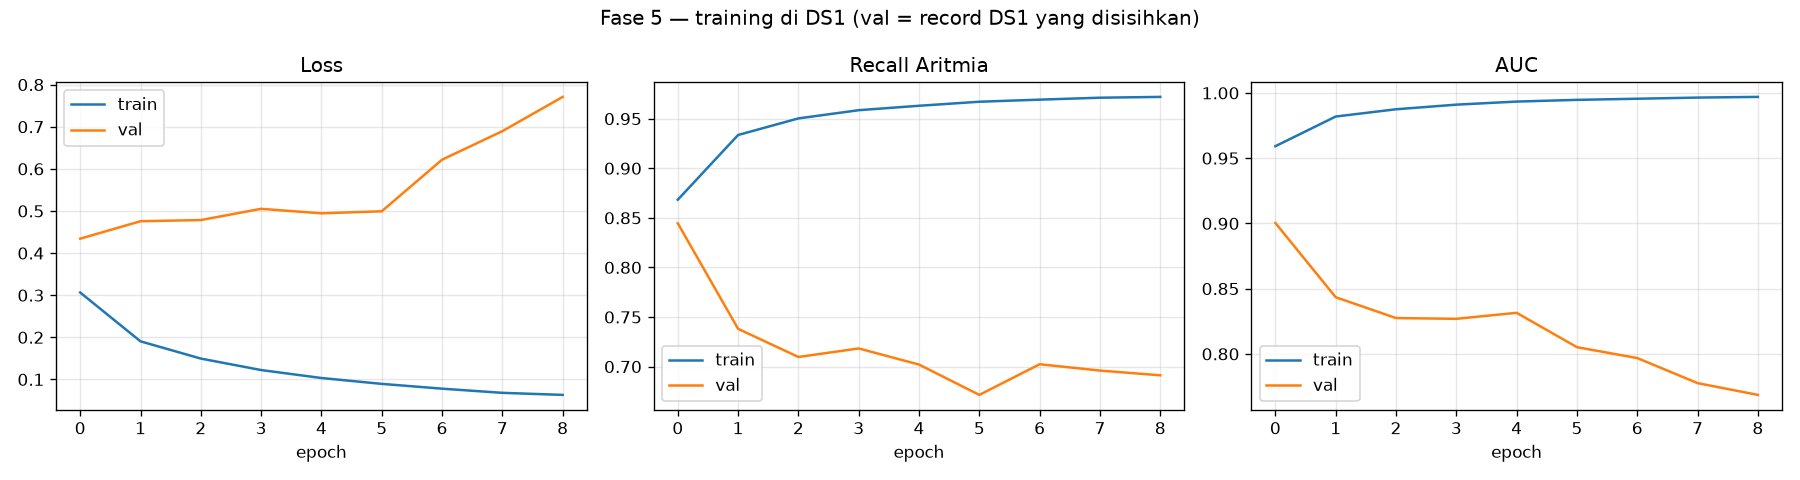
\includegraphics[width=\linewidth,keepaspectratio]{fase5_training.png}
  \caption{Kurva \textit{loss}, \textit{recall} Aritmia, dan AUC selama pelatihan model pada DS1}
  \label{fig:hasil-latih}
\end{figure}

Gambar~\ref{fig:hasil-latih} memperlihatkan kurva data latih berwarna biru yang terus membaik, sedangkan kurva VAL memburuk sejak \textit{epoch} pertama. Pada kurva VAL berwarna jingga, \textit{loss} naik dari sekitar 0,43 menjadi sekitar 0,77, dan \textit{recall} pada \textit{threshold} bawaan 0,5 turun dari sekitar 0,85 menjadi sekitar 0,69. AUC validasi memuncak sekitar 0,90 pada \textit{epoch} 0, yaitu \textit{epoch} pertama karena penomoran dimulai dari nol, lalu turun hingga sekitar 0,77 pada \textit{epoch} 8. Karena AUC validasi tidak pernah melampaui nilai \textit{epoch} 0, \textit{early stopping} mengembalikan bobot \textit{epoch} 0, dan model yang dipakai adalah hasil satu \textit{epoch} pelatihan. Penyebabnya diduga jumlah langkah gradien, karena augmentasi tiga salinan membuat satu \textit{epoch} berisi 1.905 langkah, yaitu 121.857 baris dibagi ukuran \textit{batch} 64, yang sudah cukup bagi 6.417 parameter untuk menyesuaikan diri dengan data latih.

\textit{Threshold} kemudian dipilih dari \textit{sweep} 0,05 sampai 0,95 pada VAL dengan kriteria F1 maksimum dan \textit{recall} sebagai penentu bila selisih F1 kurang dari 0,005. Nilai 0,80 memberi F1 VAL tertinggi sebesar 0,6917 dan 0,85 memberi 0,6886 dengan selisih kurang dari 0,005. Keduanya karena itu dibandingkan dengan \textit{recall}, dan 0,80 menang dengan 0,6539 dibandingkan 0,6141.
% sumber: gambar laporan/buku-pa/gambar/fase5_training.png (dibuka dan dibaca, sumbu epoch 0 sampai 8, biru = train, jingga = val; val loss 0,43 ke 0,77, val recall 0,85 ke 0,69, val AUC 0,90 ke 0,77); model/src/train.py (metrics.Recall dengan threshold bawaan 0,5, EarlyStopping restore_best_weights); model/docs/arsip/2026-09-19-faseG-changelog.md bagian 2 (1.905 langkah gradien per epoch, val_auc memuncak di epoch 0); 121.857 / 64 = 1.904,02 sehingga 1.905 langkah
% sumber: model/scripts/calibrate_threshold.py (sapuan 0,05-0,95 langkah 0,05, F1_TIE_MARGIN 0,005, pilih recall tertinggi di antara kandidat); model/artifacts/metrics/fase5_threshold_sweep.csv (0,80: f1 0,691724 recall 0,653920; 0,85: f1 0,688583 recall 0,614085); model/config.py THRESHOLD = 0.80

\subsubsection{Evaluasi pada DS2}

Kemampuan model diukur pada pasien yang tidak pernah dilihat saat pelatihan. Model INT8 yang dijalankan di perangkat dievaluasi pada 49.656 detak DS2 dari 22 pasien, termasuk 5.450 detak Aritmia, pada \textit{threshold} 0,80 dengan metrik pada Persamaan~\ref{eq:metrik}. Seluruh detak setiap rekaman dipakai, termasuk lima menit pertama yang pada protokol evaluasi AAMI dikecualikan sebagai periode belajar~\cite{aami_ec57_2012}. Periode belajar tidak relevan karena model tidak beradaptasi per pasien, dan pembagian \textit{inter-patient} de Chazal juga memakai rekaman penuh~\cite{dechazal_2004}. Hasilnya ditunjukkan pada Tabel~\ref{tab:hasil-ds2}, sedangkan model \textit{float32} dipakai sebagai pembanding kuantisasi.
% sumber: model/artifacts/metrics/fase6_per_record_fp32.csv (22 rekaman, jumlah n_beat 49.656, jumlah n_aritmia 5.450); model/scripts/eval_fp32.py (threshold dari config.THRESHOLD, tidak disetel di DS2)
% sumber: periode belajar 5 menit dari PhysioNet WAG "Evaluating ECG Analyzers" dan bxb (default -f 5 menit, mengacu EC38/EC57); de Chazal 2004 dan Luz 2016 Tabel 6 memakai seluruh detak DS2; docs/2026-11-01-crosscheck-metrik-bab4/klasifikasi.md butir 4

\begin{table}[!ht]
  \centering
  \caption{Hasil klasifikasi model INT8 pada DS2 dengan \textit{threshold} 0,80}
  \label{tab:hasil-ds2}
  \setstretch{1.0}
  \setlength{\tabcolsep}{4pt}
  \renewcommand{\arraystretch}{1.15}
  \small
  \begin{tabular}{>{\RaggedRight\arraybackslash}p{4.4cm}>{\raggedleft\arraybackslash}p{2.2cm}}
    \toprule
    \textbf{Metrik} & \textbf{Nilai} \\
    \midrule
    \textit{Recall} & 0,7105 \\
    \textit{Precision} & 0,6169 \\
    F1 & 0,6604 \\
    \textit{Specificity} & 0,9456 \\
    MCC & 0,6171 \\
    AUC & 0,9344 \\
    \textit{Accuracy} & 0,9198 \\
    \bottomrule
  \end{tabular}
  \par\vspace{2pt}{\footnotesize\raggedright Keterangan: TP 3.872, FN 1.578, FP 2.405, dan TN 41.801 dari 5.450 detak Aritmia dan 44.206 detak Normal. \textit{Accuracy} dilaporkan tetapi bukan acuan.\par}
\end{table}
% sumber: model/artifacts/metrics/fase6_metrics_fp32.csv (threshold 0.80, tp 3813, fn 1637, fp 2302, tn 41904, accuracy 0,920674, precision 0,623549, recall 0,699633, specificity 0,947926, f1 0,659403, auc 0,933448); 41.904 + 2.302 = 44.206 detak Normal; MCC 0,615986 dari model/artifacts/metrics/fase7_metrik_tambahan.csv (model/scripts/metrik_tambahan.py)

Model INT8 menemukan sekitar tujuh dari sepuluh detak Aritmia pada pasien yang tidak pernah dilihat saat pelatihan (Tabel~\ref{tab:hasil-ds2}). \textit{Recall} 0,7105 dicapai dengan \textit{precision} 0,6169, yang berarti sekitar 38\% alarm adalah alarm palsu, sedangkan AUC 0,9344 menunjukkan pemisahan kelas yang tidak bergantung pada \textit{threshold}. \textit{Accuracy} hanya sekitar 3 poin di atas hasil menebak Normal untuk seluruh detak dan karena itu tidak dijadikan acuan.

Per kelas AAMI, \textit{recall} kelas V, S, dan F masing-masing 0,9282, 0,4630, dan 0,0773 dari 3.219, 1.836, dan 388 detak. Angka ini dihitung ulang dengan menjalankan model INT8 pada DS2 beserta simbol AAMI-nya, dan 7 detak kelas Q tidak ditampilkan. Kelas S lemah karena bentuk kompleks QRS-nya mirip Normal dan pembedanya terletak pada waktu kedatangan serta gelombang P, yang menjadi alasan cabang ritme ditambahkan.
% sumber: fase6_metrics_fp32.csv; 41.904 + 2.302 = 44.206 detak Normal; 2.302 / (3.813 + 2.302) = 0,3765; tebak Normal 44.206 / 49.656 = 0,8902 dan 0,9207 - 0,8902 = 0,0305; per kelas dari perhitungan ulang dengan model/.venv atas model/artifacts/model_fp32.keras pada model/data/processed/test.npz, simbol dari model/data/processed/per_record/<rekaman>.npz dipetakan dengan config.AAMI_MAP, threshold 0,80 (S 806/1.836 = 0,4390, V 2.977/3.219 = 0,9248, F 26/388 = 0,0670, Q 4/7, jumlah terdeteksi 3.813 = TP)

\textit{Recall} per pasien dihitung pada 21 rekaman yang memiliki aritmia, karena rekaman 212 tidak memuat aritmia. Mediannya 0,9167 dan reratanya 0,7446, tetapi \textit{recall} tingkat detak terseret dua rekaman, yaitu rekaman 232 yang berisi 1.381 detak S dengan \textit{recall} 0,3838 dan rekaman 213 yang didominasi 362 detak F dengan \textit{recall} 0,2426. Keduanya menyumbang 83,2\% dari 1.578 detak terlewat. Keterbatasannya, \textit{epoch} dan \textit{threshold} hanya memakai VAL, tetapi ukuran \textit{window} dan jumlah salinan \textit{jitter} dipilih dari ablasi yang dinilai pada DS2. DS2 karena itu bukan tolok ukur yang tidak tersentuh untuk kedua keputusan itu, dan angkanya berpotensi sedikit optimistis.
% sumber: rerata recall per rekaman 0,740204 dari model/artifacts/metrics/fase7_metrik_tambahan.csv (statistik average EC57, 21 rekaman)
% sumber: model/.venv/bin/python atas model/artifacts/metrics/fase6_per_record_fp32.csv (aturan: hanya rekaman n_aritmia > 0, rekaman 212 n_aritmia 0 dikeluarkan; 21 rekaman, median recall 0,9167, 11 rekaman >= 0,9; 232 recall 0,3541 n_aritmia 1.381 fn 892; 213 recall 0,2246 n_aritmia 610 fn 473; 1.365 / 1.637 = 0,834; 1.381 / 5.450 = 0,253); komposisi kelas dari model/data/processed/per_record/232.npz (S 1.381, N 397) dan 213.npz (F 362, V 220, S 28); model/docs/arsip/2026-09-18-robustness-changelog.md (ablasi window dan salinan dinilai F1 DS2, threshold dari VAL)

\subsubsection{Ketahanan terhadap \textit{Error} Segmentasi}

Penyimpangan posisi R hasil detektor terhadap anotasi diukur beserta dampaknya pada model. Rangkaian yang identik dengan kode C, yaitu Pan-Tompkins, kompensasi 38 sampel, penyelarasan ke puncak dalam $\pm$25 sampel, dan pengurangan \textit{group delay} 4 sampel, dijalankan pada DS1 karena sebarannya kemudian dipakai untuk melatih. Selisih setiap deteksi terhadap anotasinya, yang disebut residu, ditunjukkan pada Gambar~\ref{fig:residu-jitter}.
% sumber: model/docs/jitter-walkthrough.md bagian 2 (rantai pan_tompkins_detect, haluskan, pair_detected, DS1 saja); firmware/include/ecg_preproc.h (ECG_PT_OFFSET 38, ECG_PT_REFINE 25, ECG_GROUP_DELAY 4)

\begin{figure}[H]
  \centering
  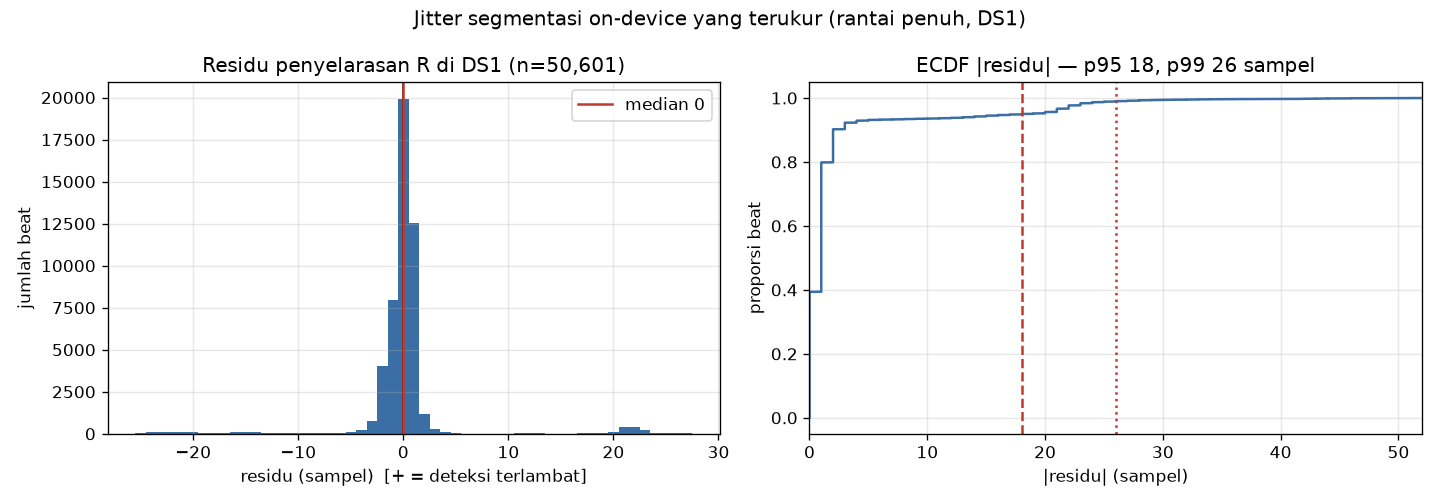
\includegraphics[width=\linewidth,keepaspectratio]{jitter_residu.png}
  \caption{Sebaran residu posisi R-\textit{peak} hasil detektor terhadap anotasi pada DS1}
  \label{fig:residu-jitter}
\end{figure}

Gambar~\ref{fig:residu-jitter} memperlihatkan histogram residu 50.601 pasangan deteksi dan anotasi pada panel kiri serta fungsi distribusi kumulatif empiris (ECDF) nilai mutlaknya pada panel kanan. Intinya tajam di sekitar median 0, yaitu 79,9\% detak meleset paling banyak 1 sampel. Ekornya berat, dengan persentil ke-95 dan ke-99 sebesar 18 dan 26 sampel yang ditandai garis vertikal, serta residu terbesar 54 sampel atau sekitar 150 ms. Ekor ini terkumpul pada rekaman berderau 108, 203, dan 207. Bentuk ini berbeda dari \textit{jitter} seragam $\pm$18 sampel pada Dias et al.~\cite{dias_2021}, karena itu augmentasi mengambil ulang residu terukur.
% sumber: gambar laporan/buku-pa/gambar/jitter_residu.png (dibuka dan dibaca); model/artifacts/metrics/jitter/residu_ds1.npy (50.601 residu, median 0, |r| <= 1 0,7985, |r| <= 2 0,9022, p95 18, p99 26, maks 54); model/artifacts/metrics/jitter/jitter_residu.csv (std 108 14,771, 203 10,792, 207 17,434); 54 / 360 = 0,150 detik; model/docs/jitter-walkthrough.md bagian 2 (paper memakai jitter seragam delta <= 18 sampel)

Pada model lama, yaitu \textit{window} 250 sampel tanpa augmentasi dengan \textit{threshold} 0,35, menggeser posisi R pada DS2 mengikuti sebaran ini menurunkan F1 dari 0,5659 menjadi 0,4534. AUC hanya turun dari 0,8866 menjadi 0,8586, jadi urutan probabilitas nyaris utuh dan yang rusak adalah titik operasinya. Pergeseran seragam 4 sampel saja sudah menurunkan F1 menjadi 0,3170, karena tiga lapisan \textit{max pooling} berukuran 2 membuat pergeseran 4 sampel setara setengah \textit{bin pooling}. Model karena itu dilatih ulang dengan dua salinan DS1 ber-\textit{jitter} empiris, dan pada model hasil latih ulang tersebut F1 dengan segmentasi detektor hanya berselisih 0,0095 dari F1 dengan segmentasi anotasi (Tabel~\ref{tab:segmentasi-deteksi}).

% sumber: rerata lima seed dari model/artifacts/metrics/jitter/sweep_jitter_dasar.csv (n 49.654 = DS2 versi window 250; delta 0: f1 0,5659 auc 0,8866; delta 4 seragam: f1 0,3170; empiris: f1 0,4534 auc 0,8586); model/docs/jitter-walkthrough.md bagian 4 (model Fase 5 threshold 0,35, kerusakan pada titik operasi); model/CLAUDE.md jebakan "Model runtuh kalau R-peak meleset 4 sampel" (stride total 8)

\subsubsection{Ablasi dan Keputusan Rancangan}

Setiap pilihan pengaturan model diputuskan dari pengukuran. Setiap varian melewati rantai yang sama, yaitu menyusun DS1 sesuai varian, melatih, mengalibrasi \textit{threshold} pada VAL, lalu mengukur DS2. Hanya satu pengaturan yang diubah per varian, dengan paling sedikit tiga \textit{seed}, dan hasilnya berupa rerata beserta setengah rentang. Selisih F1 di bawah 0,04 tidak dianggap bermakna, karena penjadwalan \textit{thread} oneDNN membuat hasil berubah walaupun \textit{seed} sama. Rerata tiga \textit{seed} konfigurasi terkunci pun bergeser dari 0,6911 menjadi 0,6535 saat diulang pada pengulangan kedua, dan F1 model akhir \textit{float32} sebesar 0,6594 berada dalam rentang pengulangan kedua, yaitu 0,6261 sampai 0,6821. Keputusan Dipilih diberikan pada varian yang dipakai dan Acuan pada varian pembanding. Keputusan Ditolak diberikan pada varian yang tidak dipakai, baik karena lebih buruk, menukar kelas yang lebih penting, maupun menambah biaya tanpa selisih bermakna. Hasil yang menentukan keputusan dirangkum pada Tabel~\ref{tab:ablasi}.
% sumber: model/docs/jitter-walkthrough.md bagian 5 (rantai ablasi, threshold per varian dari VAL, ukur DS2); model/scripts/ringkas_ablasi.py (SEED_MINIMAL 3, rerata dan setengah-rentang, AMBANG = 0.04); model/docs/arsip/2026-09-18-robustness-changelog.md bagian B2 (0,6209 vs 0,5882); keluaran ringkas_ablasi.py (w128b 0,6911, t8_lr1e3 0,6535); model/artifacts/metrics/ablasi/ablasi.csv (seed 42, 7, 13, ditambah 21, 34, 55 pada sebagian varian; t8_lr1e3 per seed 0,626084, 0,682129, 0,652266); model/artifacts/metrics/fase6_metrics_fp32.csv (f1 0,659403); model/src/dataset.py bagi_train_test (held-out sorted()[::4], sisanya ke latih); model/CLAUDE.md decision "Database LATIH" (mitdb saja)

\begin{table}[!ht]
  \centering
  \caption{Ringkasan ablasi yang menentukan keputusan rancangan, dinilai pada DS2}
  \label{tab:ablasi}
  \setstretch{1.0}
  \setlength{\tabcolsep}{3pt}
  \renewcommand{\arraystretch}{1.15}
  \small
  \begin{tabularx}{\linewidth}{>{\RaggedRight\arraybackslash}p{0.9cm}>{\RaggedRight\arraybackslash}X>{\centering\arraybackslash}p{0.9cm}>{\centering\arraybackslash}p{2.6cm}>{\raggedleft\arraybackslash}p{1.2cm}>{\raggedleft\arraybackslash}p{1.2cm}>{\centering\arraybackslash}p{1.9cm}}
    \toprule
    \textbf{ID} & \textbf{Perubahan terhadap Acuan} & \textbf{\textit{Seed}} & \textbf{F1 DS2} & \textbf{\textit{Recall} S} & \textbf{AUC} & \textbf{Keputusan} \\
    \midrule
    \multicolumn{7}{l}{\textit{Augmentasi jitter, window 90/160}} \\
    A1 & Tanpa augmentasi & 3 & 0,5660 $\pm$0,0202 & 0,2683 & 0,8870 & Acuan \\
    \textbf{A2} & \textbf{\textit{Jitter} $\times$2} & \textbf{3} & \textbf{0,6354 $\pm$0,0428} & \textbf{0,2712} & \textbf{0,9084} & \textbf{Dipilih} \\
    \midrule
    \multicolumn{7}{l}{\textit{Posisi R dalam window, jitter $\times$2}} \\
    A3 & 128/127 & 3 & 0,6775 $\pm$0,0112 & 0,4871 & 0,9394 & Ditolak \\
    A4 & 112/144 & 3 & 0,5786 $\pm$0,0311 & 0,3691 & 0,9069 & Ditolak \\
    \textbf{A6} & \textbf{128/128} & \textbf{3} & \textbf{0,6911 $\pm$0,0290} & \textbf{0,4221} & \textbf{0,9373} & \textbf{Dipilih} \\
    \midrule
    \multicolumn{7}{l}{\textit{Jumlah salinan jitter, window 128/127}} \\
    A7 & \textit{Jitter} $\times$3 & 3 & 0,6099 $\pm$0,0254 & 0,3807 & 0,9146 & Ditolak \\
    \midrule
    \multicolumn{7}{l}{\textit{Fitur HOS, window 90/160, jitter $\times$2}} \\
    A5 & $+$ HOS & 3 & 0,6150 $\pm$0,0509 & 0,3123 & 0,8882 & Ditolak \\
    \midrule
    \multicolumn{7}{l}{\textit{Fitur ritme tambahan pada A6}} \\
    A8 & $+$ rasio R-R, lebar QRS & 4 & 0,6882 $\pm$0,0233 & 0,4203 & 0,9228 & Ditolak \\
    \midrule
    \multicolumn{7}{l}{\textit{Learning rate, pengulangan kedua A6}} \\
    A9 & LR $10^{-3}$ & 3 & 0,6535 $\pm$0,0280 & 0,4473 & 0,9305 & Acuan \\
    A10 & LR $10^{-4}$ & 3 & 0,6729 $\pm$0,0483 & 0,3126 & 0,9415 & Ditolak \\
    \bottomrule
  \end{tabularx}
  \par\vspace{2pt}{\footnotesize\raggedright Keterangan: angka a/b menyatakan jumlah sampel sebelum dan sesudah R, $\times$2 dan $\times$3 adalah jumlah salinan \textit{jitter}, $\pm$ adalah setengah rentang antar-\textit{seed}, HOS adalah kurtosis dan \textit{skewness}, dan LR adalah \textit{learning rate}. Baris tebal adalah varian yang dipakai. A8 Ditolak karena F1-nya tidak berbeda bermakna dari A6 sedangkan \textit{recall} V turun. A10 Ditolak karena \textit{recall} S turun walaupun AUC naik. Hanya varian yang menentukan keputusan dengan paling sedikit tiga \textit{seed} yang ditampilkan.\par}
\end{table}
% ID varian -> tag di model/artifacts/metrics/ablasi/ablasi.csv: A1 bersih, A2 jitter, A3 w128, A4 w112, A5 hos, A6 w128b, A7 w128s3, A8 fd_mitdb_only, A9 t8_lr1e3, A10 t8_lr1e4
% sumber: keluaran model/.venv/bin/python model/scripts/ringkas_ablasi.py (F1 rerata +- setengah-rentang, recall S rerata, AUC rerata, kolom n = jumlah seed); konfigurasi per tag dari model/artifacts/metrics/ablasi/ablasi.csv (win_pre, win_post, hos, jitter, salinan, n_train); arti fb_ dan fd_ dari model/docs/arsip/2026-09-19-faseB-changelog.md bagian 1 dan 9 serta git show ad82617 (PA_RR_RATIO, PA_QRSW); vonis mengikuti model/CLAUDE.md tabel decision point ("Ukuran window", "Augmentasi jitter", "Fitur HOS", "Database LATIH", "Bentuk fitur ritme", "Learning rate"); tag dengan seed < 3 (g_diag, g_diagbase, g_lrdiag) tidak dimasukkan; baris g_lr1e4 (setara t8_lr1e4 pada batch pertama) dan fd_rr (tercakup fd_both) dikeluarkan untuk meringkas; vonis hos Ditolak mengikuti model/CLAUDE.md "Fitur HOS", w128 Ditolak karena window 128/127 tidak dipakai (255 sampel, w128b 128/128 yang terkunci)

Dua keputusan terbesar pada Tabel~\ref{tab:ablasi} adalah augmentasi \textit{jitter} dan \textit{window} 128/128. Augmentasi \textit{jitter} menaikkan F1 dari 0,5660 menjadi 0,6354 walaupun DS2 tidak diberi \textit{jitter}, jadi augmentasi bekerja sebagai regularisasi. \textit{Window} dengan 128 sampel sebelum R menaikkan F1 lebih jauh dan hampir menggandakan \textit{recall} S, sedangkan A4 yang sama-sama berpanjang 256 sampel dengan konteks sebelum R lebih pendek justru turun di bawah A2. Yang memberi manfaat karena itu adalah konteks sebelum R yang memuat gelombang P dan interval PR. Varian 128/128 setara dengan 128/127 dan dipilih karena 256 habis dibagi 8.

Biaya \textit{window} 128/128 terletak pada kelas F, yang \textit{recall}-nya turun dari 0,3084 pada acuan menjadi 0,1521. Sebagian besar penurunan itu sudah terjadi saat augmentasi \textit{jitter} ditambahkan (0,1692), jadi biaya \textit{window} sendiri kecil. Biaya ini diterima karena DS2 memuat 1.836 detak S dan hanya 388 detak F.

Fitur rasio R-R dan lebar QRS (A8) tidak menaikkan F1 secara bermakna, tetapi menurunkan \textit{recall} V dari 0,9437 menjadi 0,8983. A8 karena itu ditolak.

% sumber: tab:ablasi; model/CLAUDE.md decision "Ukuran window" (w112 sebagai isolator, konteks pre-R, gelombang P dan interval PR), "Fitur HOS", "Database LATIH", "Bentuk fitur ritme"; model/docs/arsip/2026-09-18-robustness-changelog.md bagian F1 (w128 255 sampel vs w128b 256, rantai pooling 256-128-64-32) dan F2 (3 salinan lebih buruk); rerata dari model/artifacts/metrics/ablasi/ablasi.csv (anot_recall_F bersih 0,3084, w128b 0,1521; anot_recall_V w128b 0,9437, fd_mitdb_only 0,8983); jumlah S dan F DS2 dari perhitungan ulang per kelas pada butir evaluasi DS2 (1.836 dan 388); model/docs/arsip/2026-09-19-faseB-changelog.md bagian 2 dan 9
% sumber: recall F per varian dari rerata anot_recall_F di model/artifacts/metrics/ablasi/ablasi.csv (bersih 0,308419, jitter 0,169244, w128b 0,152062; penurunan jitter 0,1392 dari total 0,1564 = 89%); varian yang tidak ditampilkan dari keluaran ringkas_ablasi.py (fb_multi 0,6419, fb_svdb_nocw 0,6223, fd_qrsw 0,6503, fd_rr 0,6853, g_swa3 0,6346, g_lr1e4 0,6827, t8_lr3e4 0,6421, semuanya di bawah varian terkunci pada kelompok batch-nya; g_diag, g_diagbase, g_lrdiag hanya 1 seed)

\textit{Learning rate} $10^{-4}$ menghasilkan pertukaran yang disengaja. AUC DS2 naik pada kedua pengulangan dan \textit{recall} F DS2 naik dari 0,1804 menjadi 0,3591, sedangkan F1 DS2 tidak berbeda bermakna. Sebaliknya, \textit{recall} S DS2 turun dari 0,4473 menjadi 0,3126. Penurunan ini bukan efek \textit{threshold}, karena pada \textit{recall} total yang disamakan, $10^{-3}$ tetap unggul pada kelas S di keenam perbandingan pada \textit{seed} 42, sedangkan penyebab pastinya belum diketahui.

\textit{Learning rate} $10^{-3}$ dipertahankan karena dua alasan. Pertama, kelas S paling bergantung pada ritme dan konteks sebelum R, dan kelas ini menjadi alasan rancangan \textit{hybrid}. Kedua, perpindahan menuntut pembuatan ulang berkas model pada \textit{firmware} beserta validasi ulang di perangkat. Model hasil satu \textit{epoch} karena itu tercatat sebagai keterbatasan yang disengaja.
% sumber: tab:ablasi (t8_lr1e3 AUC 0,9305 dan F1 0,6535, t8_lr1e4 AUC 0,9415 dan F1 0,6729, recall S t8 0,4473 dan 0,3126); keluaran ringkas_ablasi.py (w128b AUC 0,9373 dan g_lr1e4 AUC 0,9461 sebagai batch pertama, baris keduanya dikeluarkan dari tab:ablasi); selisih F1 DS2 0,6729 - 0,6535 = 0,0194 di bawah ambang 0,04; rerata anot_recall_F di model/artifacts/metrics/ablasi/ablasi.csv (t8_lr1e3 0,1804, t8_lr1e4 0,3591); model/docs/arsip/2026-09-19-faseG-changelog.md bagian 4 (threshold tetap dari VAL, uji titik operasi setara model/scripts/cek_titik_operasi.py pada DS2 test.npz hanya seed 42 pada recall total 0,65/0,70/0,80, 6 dari 6) dan bagian 8; model/CLAUDE.md decision "Learning rate" (TETAP 1e-3, biaya regen model_int8.h dan golden_ref.h serta validasi board saat HW-5 buntu)

\subsubsection{Kuantisasi INT8}

Model INT8 yang dievaluasi pada DS2 adalah hasil kuantisasi varian \textit{deploy}, yaitu DepthwiseConv1D(32) berbobot 1/32 sebagai pengganti \textit{Global Average Pooling} dengan kepala Conv1D \textit{kernel} 1. Kuantisasinya memakai \textit{post-training quantization} INT8 penuh dengan 300 sampel kalibrasi \textit{stratified} dari DS1.
% sumber: model/src/model.py build_deploy_model (kernel = panjang sesudah tiga pooling = 32, bobot 1/32, Conv1D kernel 1); model/artifacts/model_int8.tflite (tensor gap_dw [1,1,32,32]); model/config.py (REP_SAMPLES 300, INT8_IO True); model/src/quantize.py (stratified, inference_input_type dan output_type int8)

Kuantisasi memenuhi target, karena F1 model INT8 sebesar 0,6604 mencapai 100,14\% F1 model \textit{float32} sebesar 0,6594, di atas syarat 99\%. Satu-satunya metrik di bawah 99\% adalah \textit{precision}, yaitu 98,93\% nilai \textit{float32}. Penurunan itu sejalan dengan kenaikan \textit{recall}, karena probabilitas yang bergeser di sekitar \textit{threshold} menangkap lebih banyak aritmia sekaligus menambah alarm palsu.
% sumber: model/artifacts/metrics/fase7_delta.csv (f1 0,659403 / 0,660356; precision 0,623549 / 0,616855; recall 0,699633 / 0,710459); rasio int8 / float32 x 100 (f1 100,14; precision 98,93; recall 101,55; specificity 99,75; mcc 100,18; auc 100,10; accuracy 99,90); keputusan user 1 Nov 2026: tabel selisih diringkas ke kalimat

Selisih per kelas searah dengan selisih agregat, dan tidak ada kelas yang turun. \textit{Recall} kelas S, V, dan F masing-masing naik 0,0240, 0,0034, dan 0,0103. Label akhir hanya berubah pada 272 detak, yaitu 0,55\% DS2. Kedua \textit{confusion matrix} dibandingkan pada Gambar~\ref{fig:cm-ds2}.
% sumber: model/artifacts/metrics/fase7_metrik_tambahan.csv (recall_S 0,438998 / 0,462963 / +0,023965; recall_V 0,924821 / 0,928239 / +0,003417; recall_F 0,067010 / 0,077320 / +0,010309; label_berubah 272 dari 49.656 = 0,55%), model/scripts/metrik_tambahan.py; model/docs/quantize-walkthrough.md bagian 6

\begin{figure}[H]
  \centering
  \begin{minipage}{0.4\linewidth}
    \centering
    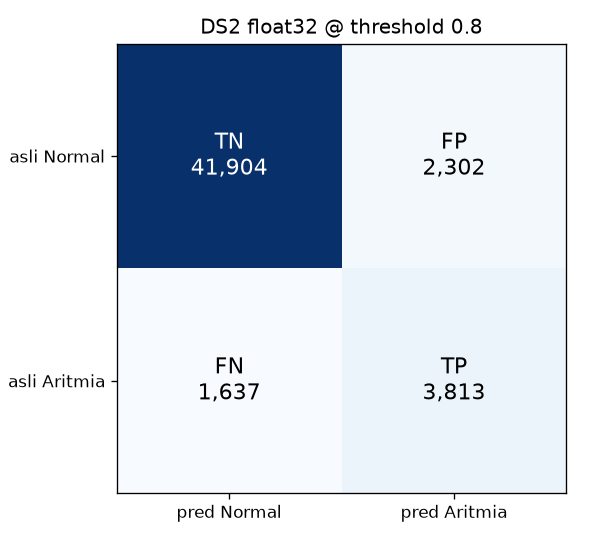
\includegraphics[width=\linewidth,keepaspectratio]{fase6_confusion_fp32.png}\\
    \small (a)
  \end{minipage}\hspace{0.05\linewidth}
  \begin{minipage}{0.4\linewidth}
    \centering
    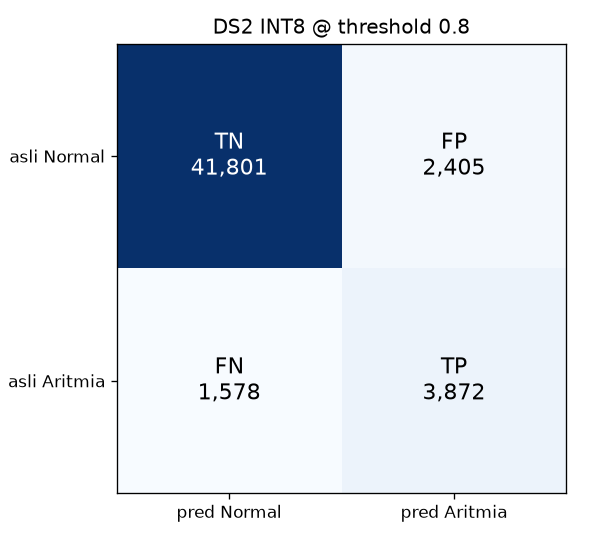
\includegraphics[width=\linewidth,keepaspectratio]{fase7_confusion_int8.png}\\
    \small (b)
  \end{minipage}
  \caption{\textit{Confusion matrix} DS2 pada \textit{threshold} 0,80, (a) model \textit{float32} dan (b) model INT8}
  \label{fig:cm-ds2}
\end{figure}

Pada Gambar~\ref{fig:cm-ds2}, baris adalah label sebenarnya dan kolom adalah prediksi. Model INT8 pada panel (b) menemukan 3.872 detak Aritmia, 59 lebih banyak daripada model \textit{float32} pada panel (a), dengan tambahan 103 FP dari 2.302 menjadi 2.405. Hasil kuantisasi ini bergantung pada varian \textit{deploy} yang dipakai. AveragePooling1D sempat dicoba sebagai pengganti, tetapi menurunkan \textit{recall} DS2 model versi lama dari 0,655 menjadi 0,528 karena operasi \textit{pooling} mewarisi skala kuantisasi masukannya.
% sumber: gambar laporan/buku-pa/gambar/fase6_confusion_fp32.png (TN 41.904, FP 2.302, FN 1.637, TP 3.813) dan fase7_confusion_int8.png (TN 41.801, FP 2.405, FN 1.578, TP 3.872), keduanya dibuka dan dibaca; 3.872 - 3.813 = 59; 2.405 - 2.302 = 103
% sumber: model/CLAUDE.md jebakan "Op pooling mewarisi skala kuantisasi input" (recall DS2 0,655 -> 0,528, skala input diwarisi)

\subsubsection{Kinerja di Perangkat}

Model INT8 harus memenuhi batas waktu dan memori di ESP32-S3. Seluruh kasus uji di \textit{board} lulus, yaitu 16 kasus pada 18 September 2026 dan 29 kasus pada 13 Oktober 2026 setelah uji perangkat dan uji integrasi ditambahkan. Latensi diukur pada 18 September 2026 atas tujuh detak acuan pada CPU 240 MHz dengan \textit{kernel} referensi TensorFlow Lite Micro tanpa ESP-NN. RAM dan Flash diambil dari laporan \textit{build} PlatformIO. Hasilnya ditunjukkan pada Tabel~\ref{tab:sumber-daya}.
% sumber: firmware/test/test_inference/test_inference.cpp test_latensi_dan_memori (rata-rata us_terpakai atas GOLDEN_RR_FIRST sampai GOLDEN_N_BEAT = 7 detak, arena_used_bytes, ESP.getFreeHeap, getCpuFreqMHz); model/docs/firmware-walkthrough.md bagian 6 (240 MHz, kernel referensi tanpa ESP-NN); model/CLAUDE.md HW-1 dan HW-6 (pio test -e esp32-s3 16/16, angka diperbarui 18 Sep 2026); git log f6042b5 dan 07a5a07 (13 Okt 2026, board 29/29; angka latensi tidak dicatat ulang)

\begin{table}[!ht]
  \centering
  \caption{Pemakaian sumber daya model INT8 dan \textit{firmware} di ESP32-S3}
  \label{tab:sumber-daya}
  \setstretch{1.0}
  \setlength{\tabcolsep}{4pt}
  \renewcommand{\arraystretch}{1.15}
  \small
  \begin{tabularx}{\linewidth}{>{\RaggedRight\arraybackslash}X>{\raggedleft\arraybackslash}p{1.8cm}>{\RaggedRight\arraybackslash}X>{\RaggedRight\arraybackslash}p{2.6cm}}
    \toprule
    \textbf{Besaran} & \textbf{Nilai} & \textbf{Kondisi Pengukuran} & \textbf{Target} \\
    \midrule
    Ukuran model INT8 (byte) & 23.488 & Format TensorFlow Lite, \textit{window} 256 & Muat di \textit{flash} \\
    Latensi inferensi per detak (ms) & 26,6 & Uji perangkat, 240 MHz, \textit{kernel} referensi, \textit{window} 256 & Lebih kecil dari interval antardetak \\
    \textit{Tensor arena} terpakai (byte) & 12.948 & Uji perangkat, alokasi 24.576 byte & Muat di SRAM \\
    \textit{Heap} bebas (byte) & 312.396 & Uji perangkat, \textit{window} 256 & Muat di SRAM \\
    RAM statis tanpa MQTT (byte) & 74.284 & \textit{Firmware} tanpa MQTT, dengan tabel \textit{replay} & Muat di memori \\
    Flash tanpa MQTT (byte) & 430.569 & \textit{Firmware} tanpa MQTT, dengan tabel \textit{replay} & Muat di memori \\
    RAM statis dengan MQTT (byte) & 121.336 & \textit{Firmware} dengan MQTT, kredensial WiFi terisi & Muat di memori \\
    Flash dengan MQTT (byte) & 887.873 & \textit{Firmware} dengan MQTT, kredensial WiFi terisi & Muat di memori \\
    \bottomrule
  \end{tabularx}
  \par\vspace{2pt}{\footnotesize\raggedright Keterangan: 23.488 byte setara 22,94 KB atau 0,36\% partisi aplikasi 6,25 MB, dan alokasi \textit{tensor arena} 24.576 byte setara 7,5\% RAM 320 KB. RAM statis 74.284 dan 121.336 byte setara 22,7\% dan 37,0\% dari RAM 320 KB, sedangkan Flash 430.569 dan 887.873 byte setara 6,6\% dan 13,5\% dari partisi aplikasi 6,25 MB.\par}
\end{table}
% sumber: 23.488 / (6,25 x 1.048.576) = 0,358%; 24.576 / (320 x 1.024) = 7,5%; flash 16 MB dari datasheet ESP32-S3-WROOM-1 (N16R8), SRAM 512 KB dari datasheet ESP32-S3; standar batas ukuran model tidak ditemukan (docs/2026-11-01-crosscheck-metrik-bab4/tinyml.md butir 4: MLPerf Tiny tidak menjadikan memori skor)
% sumber: model/docs/firmware-walkthrough.md bagian 6 (inferensi 26,6 ms, tensor arena 12.948 dari 24.576, model 22,94 KB, heap bebas 312.396, RAM 74.284 byte 22,7% dari 320 KB, Flash 430.569 byte 6,6% dari 6,25 MB); model/CLAUDE.md HW-1 (26,6 ms, 12.948 B, 312.396 B); model/docs/firmware-walkthrough.md bagian 6 dan model/docs/mqtt-walkthrough.md bagian 7 (build firmware utama dengan MQTT dan kredensial terisi: RAM 37,0% 121.336 B, Flash 13,5% 887.873 B; angka tanpa kredensial tidak dipakai; nilai lama 36,9% 121.008 B dan 881.861 B diperbarui 13 Okt 2026); firmware/src/klasifikasi.cpp ARENA_N = 24 * 1024; laporan/buku-pa/bab/bab3.tex tab:pengujian-model (target)

Seluruh besaran pada Tabel~\ref{tab:sumber-daya} memenuhi target, jadi model INT8 layak dijalankan secara \textit{on-device} tanpa \textit{cloud}. Latensi 26,6 ms setara paling banyak 13,3\% dari periode refraktori detektor 200 ms, yaitu interval antardetak terpendek, dan sekitar 4,4\% waktu CPU untuk inferensi saja pada laju \textit{replay} sekitar 1,6 detak per detik. \textit{Tensor arena} terpakai 52,7\% dari alokasinya.

RAM statis naik dari 22,7\% menjadi 37,0\% dan Flash dari 6,6\% menjadi 13,5\% karena tumpukan WiFi dan klien MQTT ikut di-\textit{link}. Angka ini hanya sah bila kredensial WiFi terisi. Keterbatasannya, latensi diukur tanpa WiFi aktif.
% sumber: tab:sumber-daya; firmware/include/ecg_preproc.h ECG_PT_REFRACTORY 72 sampel = 200 ms pada 360 Hz dan model/config.py PT_REFRACTORY_MS 200; 26,6 / 200 = 0,133; model/CLAUDE.md status HW-7 Replay dan model/docs/firmware-walkthrough.md §5c (11 detak per putaran 6,67 detik = 1,65 detak per detik), 26,6 x 11 / 6.670 = 0,044; 12.948 / 24.576 = 0,527; model/docs/firmware-walkthrough.md bagian 6 (320 KB, 6,25 MB)

\section{Analisis Hasil Eksperimen}

Hasil eksperimen pada laporan tahap ini dinilai terhadap dua tujuan penelitian, yaitu jalur preprocessing \textit{real-time} dan jalur model TinyML \textit{on-device}. Status Tercapai diberikan bila seluruh target pada rencana pengujian terukur dan terpenuhi, sedangkan Sebagian tercapai diberikan bila ada target yang belum terukur. Kedua jalur berstatus Tercapai. Penilaian per target dirangkum pada Tabel~\ref{tab:ketercapaian}.
% sumber: tab:kualitas-rekaman (4 dari 4 rekaman resmi Berhasil) melengkapi target jalur preprocessing

\begin{table}[!ht]
  \centering
  \caption{Ketercapaian tujuan penelitian}
  \label{tab:ketercapaian}
  \setstretch{1.0}
  \setlength{\tabcolsep}{3pt}
  \renewcommand{\arraystretch}{1.15}
  \small
  \begin{tabularx}{\linewidth}{>{\RaggedRight\arraybackslash}p{2.6cm}>{\RaggedRight\arraybackslash}X>{\RaggedRight\arraybackslash}X>{\centering\arraybackslash}p{2.1cm}}
    \toprule
    \textbf{Tujuan} & \textbf{Target} & \textbf{Hasil} & \textbf{Status} \\
    \midrule
    \multirow{2}{=}{Preprocessing \textit{real-time}} & Tanpa sampel hilang & Sampel hilang 0, beban 3,0\% anggaran & \multirow{2}{=}{\centering Tercapai} \\
    & Sinyal tubuh lolos indeks kualitas sinyal & 92 dari 92 jendela 10 detik, satu sesi & \\
    % sumber: bab4 tab:beban-komputasi, tab:kualitas-rekaman; target dari bab3 tab:pengujian-model dan bab4 tab:parameter-eksperimen baris d dan e
    \midrule
    \multirow{3}{=}{Model INT8 \textit{on-device}} & F1 INT8 minimal 99\% F1 \textit{float32} & 100,14\% & \multirow{3}{=}{\centering Tercapai} \\
    & Latensi di bawah interval antardetak & 26,6~ms per detak & \\
    & Muat di memori ESP32-S3 & Model 0,36\% partisi aplikasi, \textit{arena} 12.948 dari 24.576 byte & \\
    % sumber: bab4 tab:delta-int8, tab:sumber-daya; target dari bab3 tab:pengujian-model
    \bottomrule
  \end{tabularx}
  \par\vspace{2pt}{\footnotesize\raggedright Keterangan: satuan Hasil mengikuti satuan Target pada baris yang sama. F1 INT8 0,6604 terhadap F1 \textit{float32} 0,6594. Jalur \textit{pipeline edge-to-cloud} belum dinilai pada laporan tahap ini.\par}
\end{table}

Seluruh target jalur preprocessing dan jalur model, yaitu target komputasi, model, dan kualitas sinyal tubuh, terpenuhi (Tabel~\ref{tab:ketercapaian}). Target pengiriman data pada rencana pengujian \textit{pipeline}, yaitu PDSR, latensi, bufer lokal, waktu \textit{flush}, dan deduplikasi, belum dinilai karena hasil pengujiannya belum termasuk dalam laporan tahap ini.

\subsection{Analisis Jalur Preprocessing \textit{Real-Time}}

Jalur komputasi preprocessing berjalan secara \textit{real-time} di ESP32-S3. Beban rata-rata hanya 82 $\mu$s per sampel atau 3,0\% anggaran, dan sampel hilang tetap 0 walaupun puncak beban sesaat mencapai 33,4~ms (Tabel~\ref{tab:beban-komputasi}). ADC yang dibaca di ISR dan antrean 256 sampel menyerap \textit{burst} deteksi dan inferensi, dan syarat pada Tabel~\ref{tab:pengujian-model} terpenuhi.
% sumber: bab4 tab:beban-komputasi (82 us, 3,0%, 33,4 ms, sampel hilang 0, antrean 256), sec:karakteristik-data butir penyelarasan (berkas ecg_preproc.h dan model_int8.h dihasilkan otomatis)

Sinyal tubuh juga layak sebagai masukan jalur ini, karena keempat rekaman resmi dari satu sesi perekaman lolos indeks kualitas sinyal pada seluruh jendela (Tabel~\ref{tab:kualitas-rekaman}). Segmentasi hasil detektor tidak merusak klasifikasi, dengan F1 0,6499 dibandingkan 0,6594 pada segmentasi anotasi (Tabel~\ref{tab:segmentasi-deteksi}). Catatannya, beban rata-rata diukur pada sinyal \textit{replay} sepanjang 6,67 detik dengan model \textit{window} 250, dan detektor menemukan kelas S dengan \textit{sensitivity} 0,6494 (Tabel~\ref{tab:sensitivity-detektor}). Sinyal tubuh juga baru berasal dari satu subjek dan satu sesi. Karena seluruh target jalur ini terpenuhi pada pengujian yang dilakukan, jalur preprocessing dinilai Tercapai dengan cakupan tersebut dicatat sebagai keterbatasan.
% sumber: bab4 subsec:hasil-tujuan1 butir port C (rekaman 208, 6,67 detik, tanpa kelas S) dan butir alur hidup (window 250), tab:sensitivity-detektor (S 0,6494), tab:segmentasi-deteksi

\subsection{Analisis Jalur Model TinyML \textit{On-Device}}

Model INT8 berjalan secara \textit{on-device} di ESP32-S3 dalam batas waktu dan memori yang ditargetkan. Kuantisasi mempertahankan F1 pada 100,14\% nilai \textit{float32} dengan ukuran model 22,94~KB. Inferensi memakan 26,6~ms per detak atau paling banyak 13,3\% dari interval antardetak terpendek 200~ms, dan \textit{tensor arena} terpakai 12.948 dari 24.576 byte (Tabel~\ref{tab:sumber-daya}). Hasil ini bergantung pada varian \textit{deploy} berbasis DepthwiseConv1D, karena operasi MEAN pada TensorFlow Lite Micro salah hitung tanpa pesan kesalahan.
% sumber: bab4 tab:delta-int8 (+0,0108, 22,94 KB), tab:sumber-daya dan paragraf sesudahnya (26,6 ms, 13,3% dari 200 ms, 12.948 dari 24.576 byte), subsec:hasil-tujuan1 336 vs 0,973)

Kualitas klasifikasi, yang tidak memiliki ambang angka, mencapai \textit{recall} 0,7105, F1 0,6604, dan AUC 0,9344 pada model INT8 (Tabel~\ref{tab:hasil-ds2}) dengan median \textit{recall} per pasien 0,9167. Kelemahan terbesarnya adalah kelas S dengan \textit{recall} 0,4630, karena QRS-nya mirip Normal dan pembedanya terletak pada waktu kedatangan serta gelombang P. Latensi inferensi diukur tanpa WiFi aktif. Jalur model dinilai Tercapai, karena target kuantisasi, ukuran, latensi, dan memori seluruhnya terpenuhi.
% sumber: bab4 tab:hasil-ds2 (0,6996, 0,6594, 0,9334), subsec:hasil-tujuan2 butir Evaluasi DS2 (median per pasien 0,9167, recall S 0,4390, alasan QRS mirip Normal), butir Konsumsi Daya (INA219 belum dirakit di sisi baterai), paragraf sesudah tab:sumber-daya (latensi tanpa WiFi aktif)

\subsection{Perbandingan dengan Penelitian Terkait}

Perbandingan dibatasi pada penelitian terkait yang skema evaluasinya diketahui, yaitu Zambrano-de la Torre et al.~\cite{zambrano_2026} dan penelitian pendahulu~\cite{mulyawan_2026} yang memakai platform sensor dan \textit{dashboard} yang sama. Protokol ketiganya disandingkan pada Tabel~\ref{tab:perbandingan-protokol}.

\begin{table}[!ht]
  \centering
  \caption{Perbandingan protokol evaluasi dengan penelitian terkait}
  \label{tab:perbandingan-protokol}
  \setstretch{1.0}
  \setlength{\tabcolsep}{3pt}
  \renewcommand{\arraystretch}{1.15}
  \small
  \begin{tabular}{>{\RaggedRight\arraybackslash}p{2.3cm}>{\RaggedRight\arraybackslash}p{2.0cm}>{\RaggedRight\arraybackslash}p{2.5cm}>{\RaggedRight\arraybackslash}p{2.4cm}>{\RaggedRight\arraybackslash}p{3.5cm}}
    \toprule
    \textbf{Penelitian} & \textbf{Kelas} & \textbf{Pembagian Data} & \textbf{Lokasi Inferensi} & \textbf{Hasil yang Dilaporkan} \\
    \midrule
    Zambrano-de la Torre et al.~\cite{zambrano_2026} &
    Tiga kelas, yaitu N, V, dan S &
    Per detak tanpa pemisahan antarpasien pada MIT-BIH &
    Arduino UNO 8-bit, 1D-CNN INT8 &
    \textit{Accuracy}, degradasi kuantisasi $<$ 0,7\%, model $<$ 22~KB, latensi sekitar 200~ms per detak \\
    % sumber: bab2 subsec:related-zambrano2026 dan tab:perbandingan-penelitian baris 11
    Penelitian pendahulu~\cite{mulyawan_2026} &
    Atrial fibrilasi &
    Pengujian \textit{offline}, dilatih pada MIT-BIH &
    SVM di \textit{backend cloud}, ESP32 untuk akuisisi dan fitur R-R &
    \textit{Accuracy} tinggi pada pengujian \textit{offline} \\
    % sumber: bab2 subsec:related-mulyawan2026 dan tab:perbandingan-penelitian baris 12 (tanpa angka akurasi)
    Penelitian ini &
    Biner, yaitu Normal dan Aritmia &
    \textit{Inter-patient} DS1/DS2, DS2 berisi 22 pasien &
    ESP32-S3, model \textit{hybrid} INT8 \textit{on-device} &
    INT8 pada DS2 \textit{recall} 0,7105, F1 0,6604, AUC 0,9344, \textit{accuracy} 0,9198, model 22,94~KB, latensi 26,6~ms per detak \\
    % sumber: bab4 tab:delta-int8 (INT8), tab:sumber-daya (26,6 ms), subsec:hasil-tujuan2 butir Evaluasi DS2 (22 pasien)
    \bottomrule
  \end{tabular}
\end{table}

Angka ketiga penelitian pada Tabel~\ref{tab:perbandingan-protokol} tidak dapat dibandingkan langsung karena kelas, pembagian data, dan metriknya berbeda. Pembagian per detak membuat detak dari pasien yang sama dapat muncul di himpunan latih dan uji, sedangkan DS2 berisi 22 pasien yang tidak pernah dilihat saat pelatihan. Latensi juga tidak dibandingkan karena Arduino UNO 8-bit dan ESP32-S3 berbeda kelas. Pada sisi metrik, 89,0\% detak DS2 berlabel Normal, jadi menebak Normal untuk seluruh detak sudah memberi \textit{accuracy} sekitar 0,89. \textit{Accuracy} model INT8, yaitu 0,9198, hanya sekitar 3 poin di atasnya (Tabel~\ref{tab:hasil-ds2}). \textit{Accuracy} pada data setimpang ini belum menunjukkan kemampuan mendeteksi aritmia, karena itu hasil penelitian ini dilaporkan melalui \textit{recall}, F1, dan AUC.
% sumber: bab4 sec:parameter-eksperimen (89,0%, sekitar 0,89), subsec:hasil-tujuan2 butir Evaluasi DS2 (accuracy 0,9207 sekitar 3 poin di atas tebak Normal), tab:delta-int8 (0,9207 dan 0,9198)

Penelitian pendahulu mendeteksi atrial fibrilasi dengan SVM di sisi \textit{cloud}~\cite{mulyawan_2026}. Penelitian ini melanjutkannya dengan memindahkan klasifikasi per detak ke ESP32-S3. Protokol \textit{inter-patient} disadari membuat angka penelitian ini tampak lebih rendah daripada \textit{accuracy} pada pembagian per detak~\cite{xiao_2023}, dan angka DS2 pun berpotensi sedikit optimistis karena DS2 dipakai menilai ablasi \textit{window} dan \textit{jitter}. Penelitian ini karena itu tidak mengklaim \textit{accuracy} yang lebih tinggi. Yang diklaim adalah evaluasi yang lebih ketat terhadap pasien baru dan inferensi yang berjalan langsung di perangkat.
% sumber: bab2 subsec:related-mulyawan2026 (SVM di backend cloud, AFib); bab4 tab:sumber-daya (26,6 ms), subsec:hasil-tujuan2 butir Evaluasi DS2 (DS2 menilai ablasi window dan jitter, berpotensi sedikit optimistis), tab:uji-kesetaraan-tahap

\subsection{Keterbatasan dan Status \textit{Proof of Concept}}

Walaupun jalur komputasi dan model INT8 telah terukur di perangkat, sistem ini berstatus \textit{proof of concept} di lingkungan non-klinis dan bukan alat diagnosis, dengan keterbatasan yang diuraikan pada butir berikut.
\begin{enumerate}
  \item Rekaman perangkat berasal dari satu subjek sehat, yaitu penulis, dan variasi sinyal antarindividu belum terwakili.
  \item Rekaman sinyal tubuh resmi berasal dari satu sesi dengan empat rekaman yang seluruhnya memenuhi kriteria (Tabel~\ref{tab:kualitas-rekaman}), dan variasi antarsesi belum terwakili.
  \item Model hanya biner dan tidak menamai jenis aritmia.
  \item \textit{Recall} kelas S masih rendah. \textit{Learning rate} $10^{-3}$ tetap dipakai demi kelas S karena $10^{-4}$ menurunkan \textit{recall} S DS2 dari 0,4473 menjadi 0,3126 walaupun AUC naik (Tabel~\ref{tab:ablasi}), dengan konsekuensi model akhir hasil satu \textit{epoch}.
  \item Angka DS2 berpotensi sedikit optimistis karena DS2 ikut menilai ablasi \textit{window} dan \textit{jitter}.
  \item Gerbang kualitas dengan sinyal tubuh diuji pada satu subjek, dan transisi fase pada kontak baik diamati pada perangkat tanpa log serial.
  \item Deteksi R-\textit{peak} pada sinyal tubuh belum divalidasi terhadap perangkat ECG acuan, jadi hasil akuisisi berupa status fungsional dan bukan akurasi.
\end{enumerate}
% sumber: bab4 sec:karakteristik-data butir data primer, tab:kualitas-rekaman, tab:ablasi (0,4473 dan 0,3126) dan butir Ablasi (satu epoch), butir Evaluasi DS2 (DS2 ikut menilai ablasi window dan jitter, berpotensi sedikit optimistis), subsec:hasil-tujuan1 butir Gerbang Kalibrasi dan butir Segmentasi (0,6661 menjadi 0,5656, window 250)

Sebagian besar keterbatasan tersebut berkaitan dengan cakupan uji, bukan dengan jalur komputasi, dan arah pengembangannya dirangkum sebagai saran pengembangan.

\chapter{Penutup}

\section{Kesimpulan}

Penelitian ini membangun sistem monitoring detak jantung single-lead berbasis \textit{edge computing} dengan model CNN \textit{hybrid} INT8 yang berjalan \textit{on-device} pada ESP32-S3. Preprocessing sinyal ECG dan klasifikasi aritmia dijalankan di perangkat, sedangkan \textit{pipeline} MQTT dengan bufer lokal di PSRAM untuk mengirim hasil klasifikasi per detak telah dirancang. Berdasarkan perancangan, implementasi, dan eksperimen yang telah dilakukan, kesimpulan terhadap tujuan yang hasilnya dilaporkan pada tahap ini diuraikan sebagai berikut.

Preprocessing di ESP32-S3 berjalan secara \textit{real-time}. Beban rata-rata hanya 82~$\mu$s per sampel atau 3,0\% anggaran waktu tanpa sampel yang hilang, sedangkan puncak beban sesaat 33,4~ms diserap oleh ADC yang dibaca di dalam rutin interupsi (ISR) beserta antreannya. Segmentasi hasil detektor di perangkat memberi F1 0,6499 dibandingkan 0,6594 pada segmentasi anotasi. Sinyal tubuh dari AD8232 juga layak sebagai masukan, karena keempat rekaman resmi dari satu sesi perekaman lolos indeks kualitas sinyal pada seluruh jendela 10 detik. Gerbang kalibrasi berbasis kontak elektroda membuka pemantauan sekitar 60 detik setelah kontak baik dan menahan detak selama kontak buruk. Seluruh target jalur preprocessing karena itu terpenuhi.
% sumber: bab4 tab:beban-komputasi, tab:segmentasi-deteksi, tab:kualitas-rekaman (4 dari 4 Berhasil), subsec:hasil-tujuan1 butir Gerbang Kalibrasi dan Kualitas Sinyal (sekitar 60 detik, kontak buruk ditahan), tab:ketercapaian (preprocessing Tercapai)

Model INT8 pada DS2 yang berisi 22 pasien yang tidak terlihat saat pelatihan mencapai \textit{recall} 0,7105, F1 0,6604, dan AUC 0,9344. F1 tersebut 100,14\% F1 model \textit{float32}, dengan ukuran model 22,94~KB. Inferensinya di ESP32-S3 memakan 26,6~ms per detak dengan \textit{tensor arena} 12.948 byte. Karena itu target kuantisasi, latensi, dan memori terpenuhi tanpa ketergantungan pada \textit{cloud}. Kelemahan model terletak pada kelas S dengan \textit{recall} 0,4630 pada DS2.
% sumber: bab4 tab:hasil-ds2, tab:delta-int8, tab:sumber-daya, subsec:hasil-tujuan2 butir Evaluasi DS2 (recall S 0,4390) dan butir Konsumsi Daya, tab:ketercapaian

Selain ketercapaian tujuan, penelitian ini menghasilkan dua temuan teknis yang tidak terlihat dari rancangan awal.
Pertama, augmentasi \textit{jitter} yang meniru \textit{error} detektor sendiri bekerja sebagai regularisasi. Residu detektor Pan-Tompkins pada DS1 berbentuk inti yang tajam dengan ekor yang berat, berbeda dari \textit{jitter} seragam yang dipakai penelitian terdahulu. Karena itu augmentasi mengambil sampel dari residu terukur tersebut. Pada ablasi tiga \textit{seed}, F1 DS2 naik dari 0,5660 menjadi 0,6354 walaupun DS2 sendiri tidak diberi \textit{jitter}, sehingga manfaatnya bukan sekadar simulasi kondisi lapangan. Catatannya, DS2 ikut menilai ablasi ini. Kenaikan tersebut karena itu berpotensi sedikit optimistis. Implikasinya, konstanta empiris dari penelitian lain sebaiknya diukur ulang pada detektor sendiri sebelum diadopsi.
% sumber: bab4 tab:ablasi baris bersih dan jitter (0,5660, 0,6354, tiga seed), subsec:hasil-tujuan2 butir Ketahanan terhadap Error Segmentasi (residu inti tajam dan ekor berat, berbeda dari jitter seragam Dias) dan butir Ablasi (DS2 tidak diberi jitter, regularisasi), butir Evaluasi DS2 (DS2 ikut menilai ablasi, berpotensi sedikit optimistis)

Kedua, telemetri akuisisi dapat menyesatkan, sehingga kualitas sinyal tidak boleh dinilai dari keberadaan R-\textit{peak}. Detektor Pan-Tompkins memakai ambang adaptif terhadap sinyal yang ada dan tetap melaporkan R-\textit{peak} ketika biopotensial sudah hilang. Tanpa elektroda dan tanpa \textit{replay}, perangkat mengeluarkan sekitar 2 detak per detik dengan 57\% di antaranya diklasifikasi Aritmia. \textit{Flag lead-off} AD8232 pun dapat dipenuhi oleh satu jalur impedansi rendah saja dan karena itu tidak menjamin adanya sinyal. Sebaliknya, ayunan sinyal ECG yang kuat tetap tinggi ketika kontak elektroda memburuk. Penentu kualitas yang benar karena itu adalah gabungan status \textit{lead-off}, ayunan ADC absolut, dan dengung 50 Hz, dan gabungan inilah yang dipakai sebagai gerbang kualitas di perangkat.
% sumber: bab4 subsec:hasil-tujuan1 butir Akuisisi Sinyal Tubuh (perangkat tanpa elektroda sekitar 2 detak per detik, 57% Aritmia, ambang sekitar 150 count, ayunan absolut sebagai gerbang kualitas); bab2 subbab AD8232 (lead-off cukup dipenuhi satu jalur impedansi rendah); model/CLAUDE.md jebakan "Tanpa elektroda, alat mengarang aritmia\"

Secara keseluruhan, jalur preprocessing \textit{real-time} dan jalur model TinyML \textit{on-device} tercapai (Tabel~\ref{tab:ketercapaian}). Jalur \textit{pipeline edge-to-cloud} yang resilien telah dirancang, dan pengujiannya dilaporkan pada tahap berikutnya. Sistem ini berstatus \textit{proof of concept} di lingkungan non-klinis dan bukan alat diagnosis.

\section{Saran}

Berdasarkan keterbatasan sistem dan pekerjaan yang tersisa, saran pengembangan selanjutnya diuraikan pada butir berikut.
\begin{enumerate}
  \item \textbf{Validasi pada subjek yang lebih beragam.} Rekaman sinyal tubuh perlu diperluas ke lebih banyak subjek dan sesi, sebaiknya disertai alat acuan detak jantung, agar variasi sinyal antarindividu terwakili. Pada sinyal tubuh tersebut, gerbang kalibrasi berbasis kontak elektroda perlu diuji ulang dengan transisi fase yang tercatat sebagai log, termasuk ambang dengung yang dapat berbeda antarsubjek dan antarruangan.
  % sumber: bab4 subsec:analisis-keterbatasan butir 1, 2, dan 6; subsec:hasil-tujuan1 butir Gerbang Kalibrasi dan Kualitas Sinyal (satu subjek, transisi kontak baik tanpa log serial; ambang dengung 500 dari tiga sesi satu subjek)
  \item \textbf{Pengujian \textit{pipeline edge-to-cloud}.} Jalur \textit{pipeline} MQTT dengan bufer lokal di PSRAM telah dirancang, dan hasil pengujiannya belum termasuk dalam laporan tahap ini. Pengujian berikutnya menilai PDSR, median latensi \textit{end-to-end}, bufer lokal tanpa \textit{overflow}, waktu \textit{flush}, dan deduplikasi terhadap target pada Tabel~\ref{tab:pengujian-pipeline}, termasuk skenario putus koneksi dan tampilan data pada \textit{dashboard} ThingsBoard. Pengujian ini juga sebaiknya memakai sinyal tubuh, bukan hanya sinyal \textit{replay}.
  % sumber: bab3 tab:pengujian-pipeline (enam target); bab4 tab:parameter-eksperimen kategori f; hasil pipeline dibuang dari progres-pa-1 atas keputusan user 1 Nov 2026, tetap ada di laporan/buku-pa/bab/bab4.tex subsec:hasil-tujuan3
  \item \textbf{Peningkatan deteksi kelas S.} Dugaan bahwa periode refraktori 200~ms memblokir detak S yang prematur dan menekan \textit{sensitivity} detektor kelas S ke 0,6494 perlu diuji dengan mengubah periode refraktori. Pertukaran \textit{learning rate} $10^{-3}$ terhadap $10^{-4}$ pada Tabel~\ref{tab:ablasi} juga dapat ditinjau ulang bila prioritas kelas berubah. Konsekuensinya, model pada \textit{firmware} dibuat ulang serta divalidasi ulang di perangkat.
  % sumber: bab4 tab:sensitivity-detektor (S 0,6494) dan butir Segmentasi di Perangkat (dugaan periode refraktori), subsec:hasil-tujuan2 butir Ablasi (learning rate)
  \item \textbf{Perangkat \textit{wearable}.} Rakitan saat ini perlu dipindahkan ke PCB yang menyatukan seluruh modul, lalu dikemas agar perangkat dapat dipakai secara portabel. Klasifikasi juga dapat diperluas dari biner menjadi penamaan jenis aritmia bila aturan penamaannya dapat dinilai pada data validasi.
  % sumber: hardware/mainboard (PCB satu papan dengan catu baterai dan INA219); firmware/README.md bagian Rangkaian catu baterai; model/docs/README.md "Eksperimen yang tidak diadopsi" (aturan penamaan V/S tidak lolos sertifikasi VAL)
\end{enumerate}


% --- DAFTAR PUSTAKA ---
\cleardoublepage
\phantomsection
\addcontentsline{toc}{chapter}{DAFTAR PUSTAKA}
\bibliography{referensi}

\end{document}
